\documentclass[a4paper,12pt,twoside]{report}

\usepackage{fontspec}
\usepackage{xunicode}
\usepackage{xltxtra}
\usepackage{xgreek}
\usepackage{csquotes}
\usepackage{placeins}

\raggedbottom
\onecolumn

\usepackage{graphicx,amsfonts,psfrag,fancyhdr,layout,subfigure}
\usepackage{multirow}
\usepackage{longtable}
\usepackage{array}

\usepackage[toc,page]{appendix}
\renewcommand{\appendixtocname}{Παραρτήματα}
\renewcommand{\appendixname}{Παράρτημα}
\renewcommand{\appendixpagename}{Παραρτήματα}

\setmainfont[Mapping=tex-text]{GFS Artemisia}

\usepackage[style=numeric, bibstyle=numeric, hyperref=true, backref=true, alldates=terse, indexing=false, backend=bibtex]{biblatex}
\addbibresource{Bibliography.bib}

\usepackage{index}
\usepackage[columns=2]{idxlayout}
\newindex{default}{idx}{ind}{Ευρετήριο}

\usepackage{hyperref}

\usepackage[acronym, toc, translate=true]{glossaries}
\newglossary[trt]{translatedTerms}{trr}{trn}{Λεξικό αγγλικών όρων}
\loadglsentries{acronyms.tex}
\loadglsentries{glossary.tex}
\loadglsentries[translatedTerms]{translatedTerms.tex}
\renewcommand{\glossaryname}{Γλωσσάρι}
\renewcommand{\acronymname}{Συντομογραφίες}
\makeglossaries

% Set equal margins on book style
\setlength{\oddsidemargin}{53pt}
\setlength{\evensidemargin}{53pt}
\setlength{\marginparwidth}{57pt}
\setlength{\footskip}{30pt}

%%%%%%%%%%%%%%%%%%%%%%%%%%%%%%%%%%%%%%%%%%%%%%%%%%%%%%%%%%%%%
%%%%%%%%%%%%%%		   								Παράμετροι	   					   %%%%%%%%%%%%%%%%%%%%
%%%%%%%%%%%%%%%%%%%%%%%%%%%%%%%%%%%%%%%%%%%%%%%%%%%%%%%%%%%%%
\newcommand{ \FirstName}{ΔΗΜΗΤΡΙΟΣ ΑΝΔΡΕΑΣ}
\newcommand{ \LastName}{ΚΑΦΕΤΖΗΣ}
\newcommand{ \FathersName}{ΚΩΝΣΤΑΝΤΙΝΟΥ}
\newcommand{ \AM}{5657}
\newcommand{ \ThesisTitle}{ΑΞΙΟΛΟΓΗΣΗ ΤΗΣ ΓΛΩΣΣΑΣ ΜΟΝΤΕΛΟΠΟΙΗΣΗΣ ΣΥΣΤΗΜΑΤΩΝ SysML ΣΤΗΝ ΑΝΑΠΤΥΞΗ ΕΝΣΩΜΑΤΩΜΕΝΩΝ ΣΥΣΤΗΜΑΤΩΝ}
\newcommand{ \FirstProfessor}{ΚΛΕΑΝΘΗΣ ΘΡΑΜΠΟΥΛΙΔΗΣ}
\newcommand{ \FirstProfessorsRank}{ΚΑΘΗΓΗΤΗΣ}
\newcommand{ \SecondProfessor}{ΚΛΕΑΝΘΗΣ ΘΡΑΜΠΟΥΛΙΔΗΣ}
\newcommand{ \SecondProfessorsRank}{ΚΑΘΗΓΗΤΗΣ}
\newcommand{ \ThesisNumber}{ΧΧΧ}
\newcommand{ \ExaminationDay}{x}
\newcommand{ \ExaminationMonth}{x}
\newcommand{ \ExaminationYear}{x}
\newcommand{ \Month}{Απρίλιος}
\newcommand{ \Year}{2011}

% Document starts here
\begin{document}

% Page numberin set to arabic
\pagenumbering{roman}
%%%%%%%%%%%%%%%%%%%%%%%%%%%%%%%%%%%%%%%%%%%%%%%%%%%%%%%%%%%%%
%%%%%%%%%%%%%%		   								 Πρώτη σελίδα  					   %%%%%%%%%%%%%%%%%%%%
%%%%%%%%%%%%%%%%%%%%%%%%%%%%%%%%%%%%%%%%%%%%%%%%%%%%%%%%%%%%%
%%%%%%%%%%%%%%%%%%%%%%%%%%%%%%%%%%%%%%%%%%%%%%%%%%%%%%%%%%%%%
	\cleardoublepage
	\phantomsection
	\addcontentsline{toc}{chapter}{Πρώτη Σελίδα}
	\label{Πρώτη σελίδα}
		\begin{flushleft}
			\textbf{
				{\large ΠΑΝΕΠΙΣΤΗΜΙΟ ΠΑΤΡΩΝ} \linebreak
				{\normalsize ΤΜΗΜΑ ΗΛΕΚΤΡΟΛΟΓΩΝ ΜΗΧΑΝΙΚΩΝ \linebreak ΚΑΙ ΤΕΧΝΟΛΟΓΙΑΣ ΥΠΟΛΟΓΙΣΤΩΝ}\linebreak
				{\small ΤΟΜΕΑΣ:}\linebreak
				{\footnotesize ΕΡΓΑΣΤΗΡΙΟ }
			}
		\end{flushleft}
		\hrulefill
	
		\begin{center}
			\textbf{{\LARGE Διπλωματική Εργασία}}\linebreak
			{\large του φοιτητή του Τμήματος Ηλεκτρολόγων Μηχανικών και\linebreak 	Τεχνολογίας Υπολογιστών της Πολυτεχνικής Σχολής του \linebreak Πανεπιστημίου Πατρών}
			\linebreak \linebreak \linebreak
			{\large  \FirstName\space του \FathersName}
			\linebreak \linebreak
			{\large Αριθμός Μητρώου:\linebreak \AM}
			\linebreak \linebreak  \linebreak
			{\large \underline{Θέμα}}
			\linebreak  \linebreak
			{\Large \textbf{ \ThesisTitle}}
			\linebreak \linebreak \linebreak
			{\large \underline{Επιβλέπων}}
			\linebreak  \linebreak
			{\large \FirstProfessor}
			\linebreak \linebreak \linebreak \linebreak
			{\large \textbf{Αριθμός Διπλωματικής Εργασίας:\linebreak \ThesisNumber}}
			\linebreak \linebreak
			{\large Πάτρα, \Month \hspace{1pt} \Year}
		\end{center}
 
%%%%%%%%%%%%%%%%%%%%%%%%%%%%%%%%%%%%%%%%%%%%%%%%%%%%%%%%%%%%%
%%%%%%%%%%%%%%		   								 Δεύτερη σελίδα					   %%%%%%%%%%%%%%%%%%%%
%%%%%%%%%%%%%%%%%%%%%%%%%%%%%%%%%%%%%%%%%%%%%%%%%%%%%%%%%%%%%
%%%%%%%%%%%%%%%%%%%%%%%%%%%%%%%%%%%%%%%%%%%%%%%%%%%%%%%%%%%%%
	\cleardoublepage
	\phantomsection
	\addcontentsline{toc}{chapter}{Δεύτερη Σελίδα}
	\label{Δεύτερη σελίδα} 
		\begin{center}
			\textbf{{\LARGE ΠΙΣΤΟΠΟΙΗΣΗ}}\linebreak \linebreak
			{\large Πιστοποιείται ότι η Διπλωματική Εργασία με θέμα}\linebreak \linebreak
			{\Large \textbf{ \ThesisTitle}}\linebreak\linebreak\linebreak
			\begin{large}
				Του φοιτητή του Τμήματος Ηλεκτρολόγων Μηχανικών και Τεχνολογίας Υπολογιστών\linebreak \linebreak \linebreak \FirstName\space\LastName  του \FathersName\linebreak \linebreak Αριθμός Μητρώου:  \linebreak \AM \linebreak \linebreak \linebreak Παρουσιάστηκε δημόσια και εξετάστηκε στο Τμήμα Ηλεκτρολόγων Μηχανικών και Τεχνολογίας Υπολογιστών στις \linebreak \ExaminationDay / \ExaminationMonth / \ExaminationYear \linebreak
			\end{large}
		\end{center}
		\vspace{3cm}
		\begin{large}
			\begin{tabular}{m{5cm} m{1cm} m{6cm}}
			Ο Επιβλέπων & & Ο Διευθυντής του Τομέα\\
			\FirstProfessor & & \SecondProfessor \\
			\FirstProfessorsRank & & \SecondProfessorsRank
			\end{tabular}
		\end{large}
		
%%%%%%%%%%%%%%%%%%%%%%%%%%%%%%%%%%%%%%%%%%%%%%%%%%%%%%%%%%%%%
%%%%%%%%%%%%%%		   								 Τρίτη σελίδα  					   %%%%%%%%%%%%%%%%%%%%
%%%%%%%%%%%%%%%%%%%%%%%%%%%%%%%%%%%%%%%%%%%%%%%%%%%%%%%%%%%%%
%%%%%%%%%%%%%%%%%%%%%%%%%%%%%%%%%%%%%%%%%%%%%%%%%%%%%%%%%%%%%
	\cleardoublepage
	\phantomsection
	\addcontentsline{toc}{chapter}{Τρίτη Σελίδα}
	\label{Τρίτη σελίδα}
		\begin{large}
			\begin{flushleft}
				\textbf{Αριθμός Διπλωματικής Εργασίας:}\linebreak \linebreak
				\textbf{Θέμα: \ThesisTitle} \linebreak \linebreak
			\end{flushleft}
			\begin{tabular}{p{6cm} p{1cm} p{6cm}}
				Φοιτητής: & & Επιβλέπων:\\
				\FirstName\space\LastName & & \FirstProfessor\\
			\end{tabular}
			\linebreak \linebreak
			\begin{flushleft}\underline{{\large Περίληψη}}	\end{flushleft}
				\paragraph{}{Από τα μέσα του 20ού αιώνα άρχισε να αναπτύσσεται η θεωρία της μηχανικής συστημάτων δίνοντας λύση σε αρκετά προβλήματα που παρουσιάζονταν στην παραγωγή. Μια από τις τελευταίες τεχνικές που αναπτύχθηκαν από τη θεωρία αυτή είναι η \glsname{Διαγραμματική Μοντελοποίηση Συστημάτων}\glsadd{Διαγραμματική Μοντελοποίηση Συστημάτων}. Χρησιμοποιώντας διάφορα διαγράμματα περιγράφουμε το σύστημα που μας ενδιαφέρει. Αναλύουμε τη δομή του, τις διάφορες καταστάσεις στις οποίες μπορεί να επέλθει, την συμπεριφορά του στο χρόνο, την αλληλεπίδραση που επιδεικνύει με το περιβάλλον κ.ο.κ.. Ανάμεσα στα εργαλεία που υλοποιούν την γραφική μοντελοποίηση είναι και η \glsname{Systems Modeling Language} (SysML) - Γλώσσα Μοντελοποίησης Συστημάτων ελληνιστί.\linebreak
				Στην παρούσα διπλωματική εργασία μελετάμε τη χρησιμότητα της διαγραμματικής μοντελοποίησης και δει της γλώσσας Sysml στην κατασκευή ενσωματωμένων συστημάτων. Θα προσπαθήσουμε να ελέγξουμε τις δυνατότητές της αναφορικά με τα ιδιαίτερα χαρακτηριστικά των συστημάτων συγκεκριμένου πεδίου. Δηλαδή θα εξετάσουμε πως μπορεί η γλώσσα αυτή να περιγράψει συστατικά όπως μικροεπεξεργαστές, αισθητήρες, ενεργοποιητές  αλλά και λογισμικό. Μπορεί η SysML να αναπαραστήσει επαρκώς την αλληλεπίδραση των δομικών αυτών στοιχείων; Επιπλέον, θα μελετηθεί η δυνατότητά της να μεταφέρει με πιστότητα και ευκρίνεια τα στοιχεία του μοντέλου σε όλους τους εμπλεκόμενους -ηλεκτρολόγους, προγραμματιστές, χρήστες κ.λ.π..
			}
		\end{large}

\newpage
\phantomsection
% Page numberin set to arabic
\pagenumbering{arabic}
% Remove parskip for toc
\setlength{\parskip}{0ex plus 0.5ex minus 0.2ex}
\addcontentsline{toc}{chapter}{Περιεχόμενα}
\tableofcontents

\newpage
\phantomsection
\addcontentsline{toc}{chapter}{Κατάλογος Σχημάτων}
\listoffigures

\newpage
\phantomsection
\addcontentsline{toc}{chapter}{Κατάλογος Πινάκων}
\listoftables




% Dutch style of paragraph formatting, i.e. no indents.
\setlength{\parskip}{1.3ex plus 0.2ex minus 0.2ex}



% Code for creating empty pages
% No headers on empty pages before new chapter
\makeatletter
	\def\cleardoublepage{
		\clearpage\if@twoside \ifodd\c@page\else
	    \hbox{}
	    \thispagestyle{plain}
	    \newpage
    	\if@twocolumn\hbox{}\newpage\fi\fi\fi
    }
\makeatother \clearpage{\pagestyle{plain}\cleardoublepage}

% Define pagestyle
\pagestyle{fancy}
\fancyhf{}
\renewcommand{\chaptermark}[1]{\markboth{ \emph{#1}}{}}

% Adjustments headers
\fancyhead[LO]{\emph{Κεφάλαιο \thechapter}}
\fancyhead[RE]{\leftmark}
\fancyfoot[LE,RO]{\thepage}

%%%%%%%%%%%%%%%%%%%%%%%%%%%%%%%%%%%%%%%%%%%%%%%%%%%%%%%%%%%%%
%%%%%%%%%%%%%%		   								 Κεφάλαιο		   					   %%%%%%%%%%%%%%%%%%%%
%%%%%%%%%%%%%%%%%%%%%%%%%%%%%%%%%%%%%%%%%%%%%%%%%%%%%%%%%%%%%
%%%%%%%%%%%%%%%%%%%%%%%%%%%%%%%%%%%%%%%%%%%%%%%%%%%%%%%%%%%%%
	\newpage
	\chapter*{Πρόλογος}
	\addcontentsline{toc}{chapter}{Πρόλογος}
	
		\paragraph{}{Ο μηχανικός ανέκαθεν είχε και έχει ως αποστολή την παραγωγή συστημάτων και την κατασκευή υλικών σωμάτων -με την ευρεία έννοια- για την ικανοποίηση αναγκών και επιθυμιών του  ανθρώπου και του κοινωνικού συνόλου. Στη σύγχρονη όμως εποχή,τα συστήματα αυτά χαρακτηρίζονται από αυξημένη πολυπλοκότητα και τα δομικά τους στοιχεία προέρχονται από πολλαπλά επιστημονικά πεδία. Το γεγονός αυτό συνδυαζόμενο με την απαίτηση για πλήρη ικανοποίηση του σκοπού παραγωγής τους, για μείωση του χρόνου παραγωγής τους, για μείωση των αποτυχιών και των δυσχερειών που παρουσιάζονται στις διάφορες φάσεις υλοποίησης καθώς και στο πέρασμα από τη μία φάση στην άλλη και τέλος λαμβάνοντας υπόψιν την απαίτηση για εύκολη βελτίωση και εξέλιξη των εν λειτουργία συστημάτων αναπτύχθηκε η έννοια του Μηχανικού Συστημάτων.
		}
		\paragraph{}{Από τα μέσα του 20ού αιώνα άρχισε να αναπτύσσεται η θεωρία της μηχανικής συστημάτων δίνοντας λύση σε αρκετά προβλήματα που παρουσιάζονταν στην παραγωγή. Μια από τις τελευταίες τεχνικές που αναπτύχθηκαν από τη θεωρία αυτή είναι η \glsname{Διαγραμματική Μοντελοποίηση Συστημάτων}\glsadd{Διαγραμματική Μοντελοποίηση Συστημάτων}. Χρησιμοποιώντας διάφορα διαγράμματα περιγράφουμε το σύστημα που μας ενδιαφέρει. Αναλύουμε τη δομή του, τις διάφορες καταστάσεις στις οποίες μπορεί να επέλθει, την συμπεριφορά του στο χρόνο, την αλληλεπίδραση που επιδεικνύει με το περιβάλλον κ.ο.κ.. Ανάμεσα στα εργαλεία που υλοποιούν την γραφική μοντελοποίηση είναι και η \glsname{Systems Modeling Language} (SysML) - Γλώσσα Μοντελοποίησης Συστημάτων ελληνιστί.
		}
		\paragraph{}{Στην παρούσα διπλωματική εργασία μελετάμε τη χρησιμότητα της διαγραμματικής μοντελοποίησης και δει της γλώσσας Sysml στην περιγραφή και κατασκευή μηχανοτρονικών συστημάτων. Θα προσπαθήσουμε να ελέγξουμε τις δυνατότητές της αναφορικά με τα ιδιαίτερα χαρακτηριστικά των συστημάτων αυτών. Δηλαδή θα εξετάσουμε πως μπορεί η γλώσσα αυτή να περιγράψει συστατικά όπως μηχανικά μέρη, μικροεπεξεργαστές, αισθητήρες, ενεργοποιητές αλλά και λογισμικό. Μπορεί η SysML να αναπαραστήσει επαρκώς την αλληλεπίδραση των δομικών αυτών στοιχείων; Επιπλέον, θα μελετηθεί η δυνατότητά της να μεταφέρει με πιστότητα και ευκρίνεια τα στοιχεία του μοντέλου σε όλους τους εμπλεκόμενους ανθρώπους -ηλεκτρολόγους, προγραμματιστές, χρήστες κ.λ.π..
		}
		
		\paragraph{Κεφάλαιο \ref{κεφ.:Εισαγωγή στα συστήματα και στα μηχανοτρονικά συστήματα} : Εισαγωγή στα συστήματα και στα μηχανοτρονικά συστήματα} {Αναλύεται η έννοια του συστήματος και το επιστημονικό πεδίο των μηχανοτρονικών συστημάτων. Επιχειρείται μία ιστορική αναδρομή στην λέξη "σύστημα" και στην έννοιες που της έχουν αποδοθεί ανά τους αιώνες δίνοντας, βέβαια, μεγαλύτερη έμφαση στον 20ό αιώνα. Την περίοδο αυτή η εμφάνιση της γενικής θεωρίας συστημάτων και η ανάπτυξη πολύπλοκων εγχειρημάτων δομούν το πεδίο του μηχανικού συστημάτων. Στη συνέχεια περιγράφονται οι σύγχρονες εξελίξεις αναφορικά με την κατασκευή συστημάτων. Αντίστοιχα, το ίδιο επιχειρείται και για τα μηχανοτρονικά συστήματα. Τέλος, παρατίθεται μία σύνοψη σκιαγραφώντας τη σύνδεση του μηχανικού συστημάτων με την παρούσα διπλωματική.
		}
		\paragraph{Κεφάλαιο \ref{κεφ.:Μοντελοποίηση συστημάτων} : Μοντελοποίηση συστημάτων} {Τεκμηριώνεται ο ορισμός της μοντελοποίησης συστημάτων και η χρησιμότητα αυτής στο μηχανικό συστημάτων. Παρουσιάζονται τα βασικά χαρακτηριστικά της τεχνικής αυτής και ο τρόπος με τον οποίο χρησιμοποιείται. Στη συνέχεια παρατίθενται οι κυριότερες μεθοδολογίες μοντελοποίησης συστημάτων με μία σύντομη ανάλυση τους.Ως λογική συνέχεια του προηγουμένου κεφαλαίου παρουσιάζονται οι κυριότερες γλώσσες  μοντελοποίησης συστημάτων με τα κυριότερα στοιχεία τους τους. Επιπλέον τεκμηριώνεται η επιλογή της SysML για την εργασία αυτή.
		}
		\paragraph{Κεφάλαιο \ref{κεφ.:Γλώσσα SyML} : Γλώσσα SyML} {Στο κεφάλαιο αυτό επιχειρείται μία αναλυτική εισαγωγή στη SysML. Με μια σύντομη εισαγωγή αναπτύσσεται η λογική και τα δομικά στοιχεία της γλώσσας. Συμπληρωματικά, επιχειρείται ιστορική αναδρομή στη γέννηση και στην εξέλιξη της. Τέλος, παρουσιάζονται εν συντομία τα διαγράμματα τα οποία αυτή χρησιμοποιεί.
		}
		\paragraph{Κεφάλαιο \ref{κεφ.:Πρώτο πεδίο εφαρμογής : MPS System} : Πρώτο πεδίο εφαρμογής : MPS System} {Αρχικά δίνεται μια γενική, αναλυτική, λεκτική περιγραφή του συστήματος Festo MPS και των υποσυστημάτων του. Ακολούθως, επιλέγεται η μεθοδολογία που θα ακολουθηθεί για την διαγραμματική περιγραφή και κατασκευή του Festo MPS. Στη συνέχεια παρατίθεται η σχεδίαση του συστήματος με τη γλώσσα Sysml και αναπτύσσονται τα μοντέλα που κατασκευάστηκαν για το σκοπό αυτό. Επιπλέον, αναλύεται και παρουσιάζεται το στάδιο κατασκευής και εν τέλει γίνεται ο έλεγχος του συστήματος.
		}
		\paragraph{Κεφάλαιο \ref{κεφ.:Συμπεράσματα} : Συμπεράσματα} {Στο κεφάλαιο αυτό αναλύονται τα συμπεράσματα που προέκυψαν από την διπλωματική εργασία. Αναλύονται τα πλεονεκτήματα και τα μειονεκτήματα που επιβεβαιώθηκαν από την εφαρμογή της Sysml καθώς και οι διαπιστώσεις του γράφοντα από την εμπειρία της κατασκευής των συστημάτων.
		}
		\paragraph{Κεφάλαιο \ref{κεφ.:Προοπτικές} : Προοπτικές} {Καταγράφονται οι προοπτικές της μοντελοποίησης συστημάτων και πιο συγκεκριμένα της γλώσσας περιγραφής Sysml όπως αυτές προκύπτουν από εργασίες επιστημόνων και μηχανικών καθώς και πώς μπορεί να εξελιχθούν τα συμπεράσματα της διπλωματικής αυτής εργασίας.
		}
		\paragraph{} {Ολοκληρώνοντας, ακολουθούν τα παραστήματα των περιπτώσεων χρήσης όπου παρατίθενται τα διαγράμματα που κατασκευάστηκαν για την υλοποίησή τους και οποιαδήποτε επιπλέον πληροφορία. Ακολουθεί ελληνόγλωσση και ξενόγλωσση βιβλιογραφία -\ref{κεφ.:Ελληνόγλωσση Βιβλιογραφία} και \ref{κεφ.:Ξενόγλωσση Βιβλιογραφία}- , γλωσσάρι \ref{κεφ.:Γλωσσάρι}, λίστα συντομογραφιών \ref{κεφ.:Συντομογραφίες}, λεξικό αγγλικών όρων \ref{κεφ.:Λεξικό αγγλικών όρων} και ευρετήριο \ref{κεφ.:Ευρετήριο}.
		}

%%%%%%%%%%%%%%%%%%%%%%%%%%%%%%%%%%%%%%%%%%%%%%%%%%%%%%%%%%%%%
%%%%%%%%%%%%%%		   								 Κεφάλαιο		   					   %%%%%%%%%%%%%%%%%%%%
%%%%%%%%%%%%%%%%%%%%%%%%%%%%%%%%%%%%%%%%%%%%%%%%%%%%%%%%%%%%%
%%%%%%%%%%%%%%%%%%%%%%%%%%%%%%%%%%%%%%%%%%%%%%%%%%%%%%%%%%%%%
	\chapter{Εισαγωγή στα συστήματα και στα μηχανοτρονικά συστήματα}
		\label{κεφ.:Εισαγωγή στα συστήματα και στα μηχανοτρονικά συστήματα}
		
		\begin{quote}
			\textit{Ἀρχὴ παιδεύσεως ἡ τῶν ὀνομάτων ἐπίσκεψις (Αντισθένης).}
		\end{quote}
		\paragraph{}{Πριν προχωρήσουμε σε οποιαδήποτε ανάλυση πρέπει να διασαφηνιστούν οι όροι σύστημα και μηχανοτρονικό σύστημα. Να αναζητηθεί η ιστορική τους προέλευση και η αναγκαιότητα από την οποία οδηγήθηκαν οι μηχανικοί του παρελθόντος στην υιοθέτηση των όρων αυτών. Σε ποια σημαινόμενα αναφέρονται οι λέξεις αυτές και πώς έχει εξελιχθεί η χρήση τους με το πέρασμα του χρόνου με σύγχρονο αποτέλεσμα τη χρήση της μοντελοποίησης για την παραγωγή τους. Οφείλουμε να κατανοήσουμε στο πληρέστερο δυνατό επίπεδο το αντικείμενο με το οποίο θα ασχοληθούμε.
		}

%%%%%%%%%%%%%%%%%%%%%%%%%%%%%%%%%%%%%%%%%%%%%%%%%%%%%%%%%%%%%
%%%%%%%%%%%%%%		   								 Ενότητα		   					   %%%%%%%%%%%%%%%%%%%%
%%%%%%%%%%%%%%%%%%%%%%%%%%%%%%%%%%%%%%%%%%%%%%%%%%%%%%%%%%%%%		
		\section{Σύστημα}
		
			\paragraph{}{Μία πρώτη προσωπική προσέγγιση του όρου "σύστημα" επιχειρείται σε ένα ευρύτερο πλαίσιο, με αφαιρετική σκοπιά ώστε να εσωκλείσουμε την ουσία του όρου.
			}
			\paragraph{Ορισμός\label{ΟρισμόςΣυστήματος(Αφαιρετικός)}}{\textbf{Σύστημα} \index{σύστημα:ορισμός}αποτελεί οποιοδήποτε υποκείμενο, οποιαδήποτε έννοια η οποία επιδέχεται ανάλυση και παράλληλα αναγνωρίζεται και επιχειρείτε η πολλαπλή θεώρηση της.
			}
			\paragraph{}{Συνοπτικά \textit{σύστημα} μπορεί να είναι οτιδήποτε έχει εσωτερική δομή ή τουλάχιστον οτιδήποτε μπορεί να χαρακτηριστεί από εσωτερική δομή, π.χ. μία φιλοσοφική σχολή-θεωρία, το σύστημα κυκλοφορίας του αίματος στον ανθρώπινο οργανισμό, το δίκτυο δορυφόρων Gps, η τηλεόραση. Επιπλέον, πρέπει να μπορεί να αναπτυχθεί υπό διαφορετικές οπτικές γωνίες, σε διαφορετικά επίπεδα. Π.χ. το δίκτυο της Δ.Ε.Η. το οποίο σύστημα αναλύεται αναφορικά με το δίκτυο διανομής, αναφορικά με το κοινωνικό αντίκτυπο που έχει σε κάθε περιοχή, αναφορικά με τις τεχνολογίες παραγωγής ρεύματος κ.λ.π.. Συμπληρώνοντας, ένα ακόμα παράδειγμα αποτελεί η πέτρα. Αυτή αποτελεί σύστημα αν και μόνο αν ληφθούν υπόψιν η εσωτερική της μοριακή δομή και η αλληλεπίδραση της με το περιβάλλον σύμφωνα με το οποίο αναλύεται η χρήση της στο φυσικό (π.χ. στήριξη φυτών κ.λ.π.) αλλά και στο ανθρώπινο (π.χ. κατασκευή σπιτιών, εμπόδιο στη διέλευση οχημάτων κ.λ.π.) επίπεδο.
			}
			
			\paragraph{}{Τονίζεται βέβαια το γεγονός ότι ως συστήματα ο μηχανικός και συγκεκριμένα ο μηχανικός συστημάτων ενδιαφέρεται για υλικά ή άυλα συστήματα, τεχνολογικώς κατασκευάσιμα. Δηλαδή για συστήματα τα οποία εφευρίσκονται από τον άνθρωπο και χρησιμοποιούνται για την εκπλήρωση αναγκών και επιθυμιών προσωπικών και κοινωνικών. Από και στο εξής θα χρησιμοποιηθεί ο ορισμός αυτός μέχρι να συγκεκριμενοποιηθεί για τον μηχανικό και για τη σύγχρονη εποχή. Αλλά ας δούμε την ιστορική εμφάνιση του όρου.
			}
		
		\subsection{Ιστορική αναδρομή}
		
			\paragraph{}{Ιστορικά, συστήματα υπήρξαν από τη στιγμή που ο άνθρωπος χρησιμοποίησε το λογισμό του για να κατασκευάσει εργαλεία και να ερμηνεύσει το περιβάλλον του. Δηλαδή, με μεθόδους συγκεκριμένες και όχι ασυνείδητα - π.χ. τυχαία ανακάλυψη της φωτιάς, τυχαία ανακάλυψη του τροχού μετά την κύλιση ενός βράχου σε πλαγιά βουνού -, με μεθόδους οργανωτικές και συστηματικές λοιπόν άρχισε να κατασκευάζει συστήματα.
			}
			
		\subsubsection{Αρχαιότητα}
			\paragraph{}{Αρχικά τα συστήματα αυτά και οι αντίστοιχες χρησιμοποιούμενες μέθοδοι βρίσκονταν σε πρωτόλεια ανάπτυξη και κυρίως χαρακτηρίζονταν από την απαίτηση για χειρωνακτική εργασία. Χαρακτηριστικά, είχε κατασκευάσει τόξα και βέλη πολλαπλών ειδών τον 62$^{ο}$ αιώνα π.Χ. \cite{ClothesMakeTheHuMan} και είχε ανακαλύψει μεθόδους για την ύφανση ρούχων τον 34$^{ο}$ αιώνα π.Χ. \cite{MiddleStoneAgeBoneToolsFromTheHowiesonsPoortLayers}. 
			}
			\paragraph{}{Κατά την πάροδο των αιώνων, με την ανάπτυξη των επιστημών και την εμβάθυνση της ανθρώπινης σκέψης κατασκεύασε περίτεχνα οικοδομήματα, μικρού και μεγάλου μεγέθους στα οποία βρίσκει άρτια εφαρμογή η μηχανική. Παραδείγματα αποτελούν ο Ναός του Παρθενώνα, η Μεγάλη Πυραμίδα του Χέοπα, οι τριήρεις αλλά και ο μηχανισμός των Αντικυθήρων \cite{ΜηχανισμόςΑντικυθήρων}. Χαρακτηριστικά επιπλέον παραδείγματα αποτελούν τα επονομαζόμενα 7 θαύματα της αρχαιότητας \cite{ΕπτάΘαύματαΑρχαίουΚόσμου} αλλά και οι εφευρέσεις του Αρχιμήδη.
			}
			\begin{figure}[hp]
					\centering
					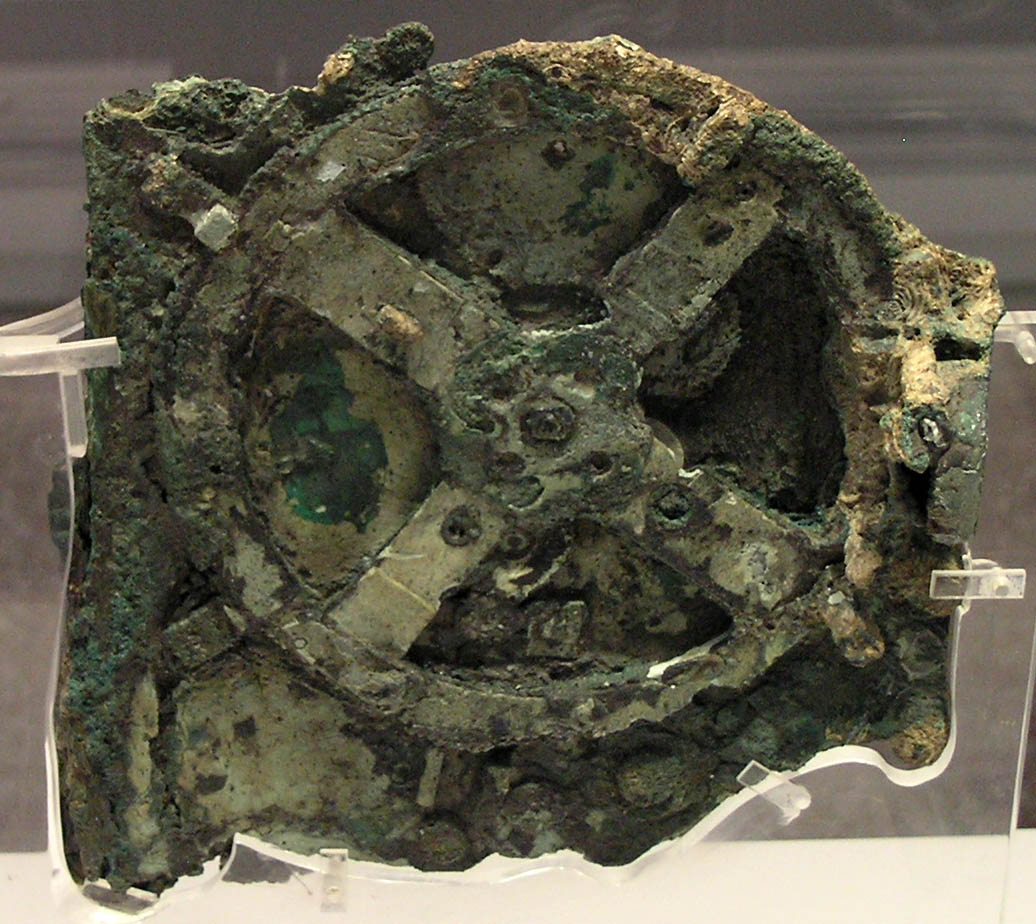
\includegraphics[scale=0.30]{Machine_Anticythere.jpg}
					\caption{Ο Μηχανισμός των Αντικυθήρων.\cite{ΜηχανισμόςΑντικυθήρωνWikipedia}}
					\label{φωτ:Ο Μηχανισμός των Αντικυθήρων}
			\end{figure}
			
			\paragraph{}{Παράλληλα ανέπτυξε θεωρίες για τον κόσμο και την ανθρώπινη κοινωνία, οι οποίες αποτελούν πλήρη φιλοσοφικά συστήματα. Μέσα σε αυτά ο κόσμος μελετάται ως Όλον με τα στοιχεία τα οποία τον αποτελούν να βρίσκονται σε αδιάκοπη αλληλεπίδραση. Ενδεικτικά αναφέρουμε τα Ορφικά κείμενα, την αντίληψη των Πυθαγορείων για το σύμπαν, τις εργασίες του Πλάτωνα και του Αριστοτέλη για κάθε τι επιστητού, τη βουδιστική και την αρχαία κινέζικη φιλοσοφία (I Ching -Το βιβλίο των αλλαγών). Τονίζεται, βέβαια, ότι η λέξη "\textit{σύστημα}" ως αυτούσια λέξη δεν απαντάται στα αναφερθέντα κείμενα\footnote{Γνωρίζουμε το ατεκμηρίωτο της δήλωσης αυτής. Κατά την προσωπική ανάγνωση μερικών βιβλίων από τα αναφερθέντα και τη διασταύρωση με τις μεταφράσεις των κινέζικων κειμένων στα αγγλικά, σε συνδυασμό με το πνεύμα της φιλοσοφίας που τα διακατέχει, δηλώνουμε ότι η λέξη "σύστημα" δεν έχει αναγνωρισθεί στα κείμενα αυτά. Το λόγο μπορούμε να τον αναζητήσουμε στην έλλειψη αναγκαιότητας για αυτήν. Η σκέψη τους ίσως να ήταν άρρηκτα συνδεδεμένη με την έννοια αυτή, σε αντίθεση με το σύγχρονο πολιτισμό ο οποίος αναγκάστηκε να την ανακαλύψει για να λύσει αρκετά προβλήματα.}.
			}
			
			\paragraph{}{Στο σημείο αυτό παραθέτουμε τον ορισμό της λέξης σύστημα, όπως αυτός διαμορφώνεται αυτή τη χρονική περίοδο. Ως λέξη αποτελεί το ουσιαστικό παράγωγο του σύνθετου ρήματος "συνίσταμαι" \cite{Dictionary.com} το οποίο ακολούθως αποτελείται από το πρόθεμα "\textbf{συν}" και τη ρίζα "\textbf{ίστημι}"\index{σύστημα:ορισμός}.
			}
			\paragraph{}{Σύμφωνα με το ετυμολογικό λεξικό του Hofmann \cite{ΕτυμολογικόΛεξικόΑρχαίαςΕλληνικής} έχουμε την εξής ετυμολογία :
			\begin{quote}
				συν : ομού μετά τινός, ομού, μαζί\\
				ίστημι (δωρ. ίσταμι) : τοποθετώ τι όρθιον
			\end{quote}
			}
			\paragraph{}{Αντίστοιχα το αγγλο-ελληνικό λεξικό του Πανεπιστημίου Tuft \cite{AGreek-EnglishLexiconHenryGeorgeLiddellRobertScott} παραθέτει τα εξής :
			\begin{quote}
				συνίστημι : A.II combine, associate, unite. A.III put together, organize, frame. A.IV bring together as friends, introduce or recommend one to another. Pass : B.II in hostile sense, to be joined, of battle. B.II.2 of persons, meet in fight, be engaged with. B.III of friends, form a league or union, band together. B.IV to come or be put together, of parts. B.V to be compact, solid, firm\footnote{[μετ. Α.ΙΙ συνδυάζω, συσχετίζω, ενώνω. Α.ΙΙΙ βάζω μαζί, οργανώνω, πλαισιώνω. Α.IV συνδέω δύο ανθρώπους ως φίλους, τους συστήνω μεταξύ τους. Παρελθοντικά : Β.ΙΙ με εχθρική έννοια, μπαίνω σε μάχη. Β.ΙΙ.2 αναφορικά με ανθρώπους, συνέρχονται σε μάχη. Β.ΙΙΙ αναφορικά με φίλους, φτιάχνω ομάδα ή ένωση. Β.IV τοποθετώ τμήματα/κομμάτια μαζί]}.
			\end{quote} 
			}
			\paragraph{}{Παρατηρείται ότι ο άνθρωπος εσωκλείει στη λέξη σύστημα θεμελιώδη χαρακτηριστικά της μηχανικής συστημάτων. Εισάγει το δίπολο μέρος - όλο και την αδυναμία μελέτης ενός υποκειμένου ανεξάρτητα από το περιβάλλον του. Μελετάει συστήματα ως τμήματα τα οποία συνδυάζονται, λειτουργούν μαζί και αποτελούν ένα στέρεο, πλήρες για το σκοπό του, σύνολο. Εν τέλει, περιγράφεται με άλλους όρους η ανάλυση ενός συστήματος σε υποσυστήματα.
			}
			
		\subsubsection{Ρώμη έως Μεσαίωνα}		
			\paragraph{}{Καθώς ταξιδεύουμε στο χρόνο από τη ρωμαϊκή στη μεσαιωνική εποχή, ο μηχανικός συνεχίζει στο ίδιο μοτίβο παραδίδοντας συστήματα όπως τα ρωμαϊκά υδραγωγεία, οι βυζαντινές εκκλησίες και τα κτήρια γοτθικού ρυθμού του μεσαίωνα. Συνεπώς, οι πρώτοι μηχανικοί συστημάτων αναγνωρίζονται οι αρχιτέκτονες και οι πολιτικοί μηχανικοί, όπως παραδέχεται και η \acrshort{INCOSE} \cite{OriginAndEvolutionOfSystemsEngineering}.
			}
			\paragraph{}{Κατά την περίοδο αυτή αναπτύσσονται κατά κόρον τα μαθηματικά, η  οπτική και η μηχανική κυρίως μέσω των οχυρωματικών έργων, των κάστρων και των πολεμικών μηχανών. Παράλληλα γνωρίζουν άνθηση η αστρονομία και η ανατομία οι οποίες διαπραγματεύονται τα δυσκολότερα συστήματα της εποχής -τα ουράνια σώματα και τον οργανισμό του ανθρώπου και των έμβιων όντων.
			}
			\begin{figure}[h]
				\centering
				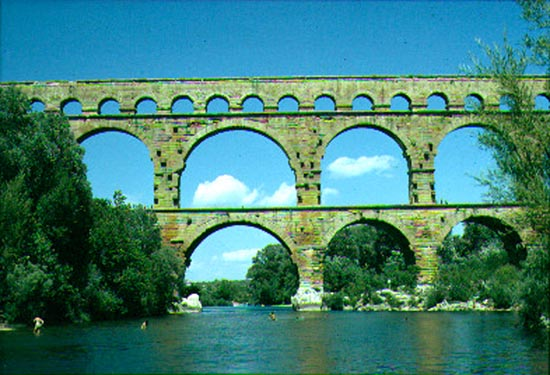
\includegraphics[scale=0.30]{pont_du_gard.jpg}
				\caption{Το ρωμαϊκό υδραγωγείο Pont du gard.\cite{PontDuGard}}
				\label{φωτ:Ο ρωμαϊκό υδραγωγείο Pont du gard}
			\end{figure}
			
			\paragraph{}{Συνεπακόλουθα, η λέξη "\textit{σύστημα}" την περίοδο αυτή συνδέεται άρρηκτα με την αστρονομία και την ανατομία. Το σύστημα ταυτίζεται με ολόκληρη τη δημιουργία, με το σύμπαν ως σύνολο πλανητών και αστρικών σωμάτων -στα ύστερα λατινικά- αλλά και με με τον έμβιο οργανισμό ως το σύνολο των ζωτικών λειτουργιών του \cite{Dictionary.com}\index{σύστημα:ορισμός}.
			}
			\paragraph{}{Επισημαίνεται ότι η λέξη "σύστημα", την εποχή αυτή, μπορεί να συνδυαστεί με τη θεοκρατική φιλοσοφική αντίληψη της εποχής, αφού αυτή πραγματεύεται κάθε πτυχή του κόσμου και της κοινωνίας. Πραγματεύεται τον κόσμο ως μία και μόνη οντότητα, του θέτει κανόνες και νόρμες : ο κόσμος είναι πεπερασμένος και φθαρτός, η σωτηρία της ψυχής είναι ο απώτερος σκοπός του ανθρώπου, η επιστήμη και η κοινωνική ζωή είναι υποτελείς στη θεολογία \cite{GeneralSystemsTheory:Skyttner2005}.
			}
		
		\subsubsection{Μεσαίωνας έως Αναγέννηση}	
			\paragraph{}{Κατά την περίοδο αυτή καθιερώθηκε ο σύγχρονος επιστημονικός τρόπος σκέψης, ο βασιζόμενος στην παρατήρηση, την ανάπτυξη θεωρίας και εν τέλει την επαλήθευση μέσω πειραμάτων.
			
			\paragraph{}{Για να συγκεκριμενοποιήσουμε την αναφορά μας στην περίοδο αυτή πρέπει να αναφέρουμε τις δύο μεγάλες σχολές που αναδύθηκαν και τοποθέτησαν τις βάσεις για την σύγχρονη επιστημονική μέθοδο. Πρώτη είναι ο \textit{ορθολογισμός}\index{ορθολογισμός}\glsadd{Ορθολογισμός} με κυριότερο εκπρόσωπο τον τον Καρτέσιο\index{Καρτέσιος}\index{Descartes Ren\'e}. Καθιέρωσε τον ορθολογισμό και τον σκεπτικισμό και ανέπτυξε μία μέθοδο σκέψης \cite{DiscourseΟnMethod:Descartes} με βασικά χαρακτηριστικά της να αποτελούν η διαίρεση των δυσκολιών που συναντά κανείς στο λογισμό του σε μικρότερα μέρη και η συλλογιστική διάταξη από τα απλούστερα στα σύνθετα\footnote{Τα "αξιώματα" της μεθόδου του είναι τα εξής \cite{ΛόγοςΠερίΤηςΜεθόδουDescartes1976} : \begin{itemize} \item Να μην προσλαμβάνεται τίποτα για αληθινό αν δεν είναι ξεκάθαρα αληθινό, αποκλείοντας τις προκαταλήψεις. \item Κάθε δυσκολία να διαιρείται σε μικρότερες μέχρι να μπορεί να λυθεί. \item Να θεωρούνται πρώτα τα απλούστερα και στη συνέχεια να γνωρίζονται τα συνθετότερα υποθέτοντας πως υπάρχει κάποια τάξη ανάμεσά τους. \item Τέλος, να επανεξετάζεται όλο το αποτέλεσμα με σκοπό να μην παραληφθεί τίποτα.\end{itemize}}. Με τη σχολή αυτή οφείλεται να αναφερθεί και η εργασία του Γαλιλαίου\index{Γαλιλαίος Γαλιλέι}\index{Galileo Galilei} του οποίου η αναλυτική μέθοδος συμβαδίζει με το δεύτερο αξίωμα της Μεθόδου του Καρτέσιου. Η δεύτερη είναι ο \textit{εμπειρισμός}\index{εμπειρισμός}\glsadd{Εμπειρισμός} ο οποίος δηλώνει ότι η πηγή και τα συστατικά της ανθρώπινης γνώσης προέρχονται από την εμπειρία που αποκτάται μέσω των αισθήσεων, είτε εξωτερικών -ακοή, όραση, αφή, οσμή, γεύση- είτε εσωτερικών -πόνος, ευχαρίστηση-.
			}
			
			\paragraph{}{Κόπτονται τα δεσμά της επιστήμης και ανεξαρτητοποιείται από την Εκκλησία και τον έλεγχο αυτής. Με βάση τον πειραματισμό και τη φιλοσοφική και μαθηματική ανάλυση επιχειρείται να καταστεί ο κόσμος κατανοητός στον ανθρώπινο λογισμό με έννοιες αντίθετες των δοξασιών και των προκαταλήψεων. Δεν υπάρχει το ά-γνωστο. Ό,τι δεν έχει εξηγηθεί αναμένει να ερμηνευθεί. Τα πάντα υπάγονται σε κανόνες και νόρμες καθορίσιμες από τον ανθρώπινο νου.
			}
		
		\subsubsection{Βιομηχανική επανάσταση έως σήμερα}		
			\paragraph{}{Η απελευθέρωση της επιστήμης ολοκληρώνεται θεωρητικά μέσα στον 19ο αιώνα\footnote{Ολοκληρώνεται λοιπόν θεωρητικά αφού οι ιδέες του διαχωρισμού θρησκείας και επιστήμης πρέπει να γίνουν κοινά αποδεκτές από ολόκληρο τον κόσμο, γεγονός το οποίο δεν έχει επιτευχθεί ούτε στη σύγχρονη εποχή.}. Ολοκληρώνεται με τη δημοσίευση της εξελικτικής θεωρίας \cite{OriginOfSpecies:Darwin1859} του Δαρβίνου\index{Darwin}\index{Δαρβίνος}\footnote{Βιβλιογραφία του Δαρβίνου : \url{http://darwin-online.org.uk/biography.html}} και των εργασιών αυτού και του Alfred R. Wallace\index{wallace Russel Alfred}\footnote{Βιβλιογραφία του Wallace : \url{http://wallacefund.info/biography-wallace}} \cite{OnTheLawWhichHasRegulatedTheIntroductionOfNewSpecies:Wallace1840}. Μέσω αυτών οι φυσικοί νόμοι του Νεύτωνα αποτελούν μέρος της ίδιας της ανθρώπινης ζωής. Γίνονται δηλαδή κομμάτι της καθημερινότητας αφού ο άνθρωπος πλέον μελετά τη ζωή του έχοντας ως εργαλεία το λογισμό, την παρατήρηση και την πρόβλεψη τη σύμφωνη με τους φυσικούς νόμους \cite{GeneralSystemsTheory:Skyttner2005}.
			}
			
			\paragraph{}{Από το 19$^{ο}$ αιώνα αρχίζει η επίσημη ιστορία της μηχανικής συστημάτων. Την περίοδο αυτή παρουσιάζονται οι πρωταρχικές θεωρητικές συλλήψεις και πρακτικές πάνω στη θεωρία συστημάτων και τοποθετούνται οι βάσεις για τον επιστημονικό τομέα που σήμερα ονομάζουμε μηχανική συστημάτων. Διαφαίνεται η διεπιστημονικότητα της θεωρίας αφού μπορούμε να εντοπίσουμε ρίζες της στη μηχανική, στη βιολογία και στη διοίκηση επιχειρηματικών οργανισμών. Θα προσπαθήσουμε να παρουσιάσουμε τα κομβικά σημεία στην εξέλιξη και στη διαμόρφωση της θεωρίας αυτής\footnote{Δεν ισχυριζόμαστε ότι η καταγραφή αυτή της ιστορίας είναι πλήρης. Πραγματικά, δεν είναι αυτός ο σκοπός που επιδιώκεται. Η προσπάθειά μας επικεντρώνεται στη διαύγαση της λέξης \textit{σύστημα} και της ιστορικής εξέλιξης της θεωρίας συστημάτων και την διαμόρφωση του μηχανικού συστημάτων. Για μια πιο λεπτομερή ιστορική ανάλυση παρακαλείσθε να ανατρέξετε στα συγγράμματα του Ludwig Von Bertalanffy \cite{TheHistoryΑndStatusΟfGeneralSystemsTheory:Bertalanffy} και \cite[κεφάλαιο: εισαγωγή]{GeneralSystemsTheory:Bertalanffy1972}, του Strijbos \cite{SystemsThinking:STRIJBOS2010}, των Pahl, Beitz και Wallace \cite[νότητα 1.1.2]{EngineeringDesignASystematicApproach:Pahl1996}, του Mindell \cite{HistoricalPerspectivesOnSystemsThinkingInEngineering}, των Gibson και Scherer \cite[ενότητα 1.8]{HowToDoSystemAnalysis:Gibson2007}, του Buede \cite{EngineeringDesignOfSystemsModelsAndMethods:Buede2011} και του Lars Skyttner \cite{GeneralSystemsTheory:Skyttner2005}.}.
			}

			\paragraph{}{Διαμορφώνεται η ιδέα στο συλλογικό φαντασιακό των ανθρώπων ότι για να ερμηνευθεί ο κόσμος, να προχωρήσουμε στην επεξεργασία πιο πολύπλοκων συστημάτων από τα ήδη θεωρούμενα και να λυθούν τα προβλήματα που παρουσιάζονται στην επιστήμη, είναι απαραίτητη μία καινούρια θεωρία σύμφυτη με τη γενικευμένη, ολιστική θεώρηση του κόσμου. Συνεπώς δεν αρκεί πρώτον, η αναλυτική μελέτη των φαινομένων που εισήγαγε ο Καρτέσιος σύμφωνα με τον οποίο για να λυθεί ένα πρόβλημα έπρεπε να διαιρεθεί σε μικρότερα επιλύσιμα προβλήματα και δεύτερον, η απομόνωση του υπό μελέτη υποκειμένου από το περιβάλλον δράσης του. Παράλληλα, αρχίζουν να εμφανίζονται συστήματα πολύπλοκα -που αφορούν το μηχανικό- που περιλαμβάνουν παραμέτρους κοινωνικούς, πολιτικούς εκτός από παραμέτρους καθαρά τεχνικούς ("μηχανικούς"). Καταγράφονται τα προβλήματα στην υλοποίηση των συστημάτων αυτών, η ανεπάρκεια των εφαρμοζομένων τεχνικών σχεδίασης και παραγωγής με απώτερη συνέπεια την τάχιστη εξέλιξη των συστημάτων και της θεωρίας σχεδίασης αυτών και με τελικό αποτέλεσμα τον ολοκληρωμένο επιστημονικό κλάδο του μηχανικού που γνωρίζουμε στην εποχή μας.
			}
			\paragraph{Η τελευταία αυτή περίοδος μπορεί να χωριστεί σε τρεις φάσεις }{με κριτήριο την ωρίμανση, τη μεθοδολογία και τις πρακτικές που χρησιμοποιούνται στο σχεδιασμό και την υλοποίηση των συστημάτων \cite{HistoricalPerspectivesOnSystemsThinkingInEngineering, OriginAndEvolutionOfSystemsEngineering}. Η πρώτη επεκτείνεται από το 19ο αιώνα μέχρι το δεύτερο παγκόσμιο πόλεμο, η δεύτερη περιλαμβάνει το δεύτερο παγκόσμιο καθώς και την περίοδο του  ψυχρού πολέμου και τέλος η τρίτη αναφέρεται στη σύγχρονη μας εποχή ξεκινώντας από το 1990.
			}
		
		\subsubsection{1800 έως δεύτερο παγκόσμιο πόλεμο}
			\paragraph{}{Συνοπτικά, μπορούμε να αναφέρουμε ότι το μονοπώλιο της αρχιτεκτονικής και της αστρονομίας πάνω στα πολύπλοκα συστήματα καταρρίπτεται και μερίδιο διεκδικούν πλέον και άλλοι επιστημονικοί τομείς. Δύο γεγονότα στιγματίζουν την περίοδο αυτή. Αφενός, η ανεξαρτητοποίηση της επιστημονικής σκέψης από τη θρησκευτική καθοδήγηση και η παγίωση των μεθόδων που αναπτύχθηκαν τους προηγούμενους αιώνες λαμβάνει καθολικές διαστάσεις στην Ευρώπη και την Αμερική. Το αποτέλεσμα της παγίωσης αυτής είναι η περαιτέρω ανάπτυξη της επιστημονικής σκέψης και η εμφάνιση σημαντικών θεωριών σε διάφορους τομείς όπως η μηχανική, η βιολογία και η ψυχολογία. Αφετέρου, με τη συντέλεση της βιομηχανικής επανάστασης\index{βιομηχανική επανάσταση} (1750 - 1850) και τη διαπίστωση για τη θετική αλλαγή που επέφερε αυτή στον τρόπο διαβίωσης, οδηγούμαστε στην κατασκευή ολοένα και πολυπλοκότερων μηχανών-συστημάτων σε ολοένα και μεγαλύτερες ποσότητες. Τα συστήματα που κυριαρχούν την περίοδο αυτή είναι το σιδηροδρομικό δίκτυο και το δίκτυο τηλεφωνικών επικοινωνιών της AT{\&}T, οι μηχανές συνεχούς και εναλλασσόμενου ρεύματος και το αντίστοιχο δίκτυο που εγκαθιστά ο Thomas Edison\index{Edison Thomas} καθώς και οι γραμμές παραγωγής των εργοστασίων του Henry Ford\index{Ford Henry}.
			}
			
			\paragraph{}{Λόγω κυρίως των δύο προαναφερθέντων γεγονότων διαμορφώνονται δύο τάσεις οι οποίες δομούν την έννοια του συστήματος και το πεδίο του μηχανικού. Οι τάσεις αυτές, ανεξάρτητες αρχικά, θα μας απασχολήσουν καθ' όλη τη διάρκεια της περιόδου αυτής αλλά και μέχρι τη σύγχρονη εποχή. Θα προσπαθήσουμε να τις ιστορήσουμε παράλληλα -διατηρώντας την χρονική δομή αυτής της ενότητας- και να δείξουμε πως αλληλοεξαρτώνται και χαρακτηρίζουν το πεδίου του μηχανικού συστημάτων. Οι δύο αυτές λοιπόν τάσεις είναι οι εξής :
			\begin{itemize}
				\item η προσπάθεια για την ανάπτυξη μιας ολιστικής θεωρίας της επιστήμης και της ανθρώπινης γνώσης. Κατά την προσπάθεια αυτή, διακρίνονται κοινά στοιχεία μεταξύ διαφορετικών επιστημονικών πεδίων για τα οποία προσπαθείται να αναχθούν σε καθολικά στοιχεία θέτοντας τις βάσεις για τη θεωρία συστημάτων.
				\item η προσπάθεια για βελτίωση της παραγωγής και συγκεκριμένα της ποιότητας των τεχνολογικών προϊόντων και της διαδικασίας παραγωγής αυτών.
			\end{itemize} 
			}
			
			\paragraph{Ολιστική θεώρηση}{Οι πρωταρχικές αναφορές για μία ολιστική θεώρηση του κόσμου, διαφορετική από την κλασσική επιστήμη προέρχονται από πεδία θεωρητικών επιστημών όπως της ιστορίας, της κοινωνιολογίας και της φιλοσοφίας αλλά και από τις θετικές επιστήμες όπως η βιολογία.
			}
			\paragraph{Hegel}{Αρχικά, αναφέρεται η παρατήρηση του D. C. Phillips\index{Phillips D.C.} σύμφωνα με τον οποίο \cite[σελ. 5]{SystemsTheoryADiscreditedPhilosophy:Phillips1969} και τον Stafford Beer\index{Stafford Beer} οι ιδέες του Hegel\footnote{Βιογραφία του Hegel : \url{http://www.iep.utm.edu/hegelsoc/\# H1}}\index{Hegel} σχετίζονται με τη θεωρία συστημάτων και προετοιμάζουν το έδαφος για αυτήν. Σε αυτο συνηγορεί και ο Von Bertalanffy στην εργασία του για την ιστορική εξέλιξη των συστημάτων \cite{TheHistoryΑndStatusΟfGeneralSystemsTheory:Bertalanffy}. Ο Hegel χρησιμοποιεί τον όρο "Απόλυτο" ("Absolute") για να δηλώσει τον κόσμο όλο και κάθε τι υπαρκτό.  Θεωρεί το Απόλυτο, τον ίδιο τον κόσμο ως ένα σύστημα τα μέρη του οποίου αλληλεπιδρούν μεταξύ τους ή σχετίζονται οργανικά.  Δήλωνε ότι αν ένα μέρος απομονωθεί από το σύστημα τότε αλλάζει η φύση του και δεν μπορούμε δια αυτού να μελετήσουμε το ίδιο το σύστημα. Συνεπώς η πραγματικότητα και ο κόσμος δεν μπορούν να μελετηθούν μόνο με την ανάλυση των μερών τους αλλά οφείλεται να ληφθούν υπόψιν και οι σχέσεις και αλληλεπιδράσεις των στοιχείων από τα οποία αποτελούνται και κυρίως με τις καινούριες ιδιότητες που τα μέρη αποκτούν όταν εισέλθουν στο ευρύτερο πεδίου του συστήματος-του υποκειμένου προς μελέτη.
			}
			\paragraph{Bogdanov}{Επίσης ο Ρώσος φιλόσοφος και επιστήμονας Alexander A. Bogdanov\footnote{Βιογραφία του Smuts : \url{http://www.newworldencyclopedia.org/entry/Alexander_Bogdanov}}\index{Phillips Bogdanov Alexander} με το έργο του "Tektologiya: vseobschaya organizatsionnaya nauka" του 1922 παρουσίασε μία πρώτη σύλληψη πάνω στη θεωρία συστημάτων\footnote{Το έργο αυτό εκδόθηκε στα ρώσικα με τίτλο "Tektologiya: vseobschaya organizatsionnaya nauka" με τον πρώτο τόμο να παρουσιάζεται το 1913, το δεύτερο το 1917 και ο τρίτος και τελευταίος το 1922. Ακολούθησε η γερμανική μετάφραση το 1926-28 και εν τέλει η αγγλική "Essays in tektology : the general science of organization" \cite{EssaysInTektology:Bogdanov1984} την οποία και έχουμε υπόψιν μας.}. Ο Bogdanov χρησιμοποίησε τη λέξη tektology\index{tektology} για να περιγράψει τη φιλοσοφική του θεωρία και με την οποία προσπαθεί να καταργήσει τη διαχωριστική γραμμή μεταξύ φιλοσοφίας, θετικών και ανθρωπιστικών επιστημών \cite{InstrumentalReasoningAndSystemsMethodologym:Mattessich1978}. Ο ίδιος περιγράφει τη λέξη "tektology" ως μία γενικευμένη μελέτη των κανόνων οργάνωσης κάθε στοιχείου της φύσης, σκέψης και πράξης. Προσπαθεί να συστηματοποιήσει της τεχνικές οργάνωσης ώστε αυτές με τη σειρά τους να αναδείξουν τη δομική συγγένεια μεταξύ ετερογενών φαινομένων, και να ανακαλύψει κοινούς νόμους στα διάφορα πεδία γνώσης \cite{AleksandrBogdanovAndSystemsTheory:Arran2000}. Δεν χρησιμοποιεί τη λέξη "σύστημα" αλλά τη λέξη "συγκρότημα"\index{συγκρότημα} ("complex"\index{complex} στην αγγλική έκδοση) με την οποία περιγράφει το συνδυασμό συστατικών σύμφωνα με κάποια δομή, τα οποία συστατικά βρίσκονται σε αλληλεπίδραση. Υποστηρίζει ότι ένα συγκρότημα μπορεί να αποτελεί συστατικό για ένα άλλο, δηλαδή υποστηρίζει την ανάλυση των συγκροτημάτων σε ολοένα και απλούστερα συστατικά. Τέλος, υποδεικνύει τη σημαντικότητα της αλληλεπίδρασης των επιμέρους συστατικών με τη φράση του "Το όλον διαχωρισμένο στα συστατικά του είναι μικρότερο από το συνδυασμό των μερών του". Εννοεί ότι το όλον το οποίο δεν μπορεί να κρατήσει τη δομή του -τις σχέσεις δηλαδή μεταξύ των μερών του- υπολείπεται από το άθροισμα των μερών του με τις μεταξύ τους σχέσεις. \cite{AleksandrBogdanovAndSystemsTheory:Arran2000}.
			}
			\paragraph{Haldane}{Αρχικά ψήγματα της θεωρίας συστημάτων μπορούν να αναζητηθούν \textit{και} στη βιολογία. Αναφορά γίνεται από τον D. C. Phillips στο \cite[σελ. 8]{SystemsTheoryADiscreditedPhilosophy:Phillips1969} στον J.S. Haldane\footnote{Βιογραφία του J.S. Haldane : \url{http://www.oxfordshireblueplaques.org.uk/plaques/haldane.html}}\index{Haldane J.S.} (1860 - 1936) ο οποίος παρατήρησε ότι η μηχανιστική αντίληψη του αιτίου-αποτελέσματος καθώς και η αναλυτική μέθοδος της διαίρεσης σε μέρη για τη μελέτη ενός υποκειμένου, δεν επαρκούν για τη μελέτη των σύγχρονων νεο-ανακαλυφθέντων  φαινομένων που υπάγονται στην βιολογία, μοριακή βιολογία και στη φυσιολογία. Ο ίδιος στο \cite[σελ. 33]{LifeAndMechanism:Haldane1884} γράφει \begin{quote}What is true of the organism and its surroundings looked at as wholes in relation to one another, applies of course equally when the organism is looked at as made up of a number of separate parts. These parts stand to one another and to the surroundings, not in the relation of cause and effect, but in that of reciprocity\glsadd{reciprocity}. The parts of an organism and its surroundings thus form a system, any one of the parts of which constantly acts on the rest, but only does so, qua part of the system, in so far as they at the same time act on it.\footnote{Μετάφραση στα ελληνικά : [σ.τ.μ. Ο Haldane, παρατηρώντας τους έμβιους οργανισμούς και παραθέτοντας ως παραδείγματα το σκουλήκι που επιλέγει με προσοχή τα φύλλα με τα οποία καλύπτει την τρύπα του και την ανάπλαση κομμένων μερών από το σώμα της σαλαμάνδρας, καταλήγει στο γεγονός ότι οι έμβιοι οργανισμοί και το συγκεκριμένο περιβάλλον στο οποίο ζουν βρίσκονται σε αλληλεπίδραση και οι ίδιοι οργανισμοί επιδεικνύουν τη συγκεκριμένη συμπεριφορά μόνο και μόνο επειδή βρίσκονται στο συγκεκριμένο περιβάλλον.] Η θεώρηση του οργανισμού και του περιβάλλοντος του ως ένα συμπεριλαμβανομένων και των μεταξύ τους σχέσεων, εφαρμόζεται ισοδύναμα και στον ίδιο τον οργανισμό θεωρούμενος ότι αυτός απαρτίζεται από ξεχωριστά μέρη. Μεταξύ των μερών αυτών και μεταξύ αυτών και του περιβάλλοντος υπάρχουν σχέσεις όχι αιτίου-αποτελέσματος αλλά αμοιβαίας αλληλοπάθειας. Συνεπώς τα μέρη του οργανισμού και του περιβάλλοντός του αποτελούν σύστημα με το κάθε μέρος του οποίου να δρα πάνω στα υπόλοιπα, και δρα μόνο και μόνο όντας μέρος του συστήματος αυτού, σε τέτοια έκταση που υποδηλώνεται από την ταυτόχρονη επίδραση των υπολοίπων μερών πάνω του.}\end{quote}
			}
			\paragraph{C. Smuts}{Τον Haldane ακολουθούν και άλλοι όπως οι C. Lloyd Morgan, Edmund Montgomery, E. R. Russell και ο C. Smuts. Ο τελευταίος φιλοσοφώντας πάνω στον κόσμο και στη φύση παρατηρεί το γεγονός ότι τα χαρακτηριστικά μιας οντότητας, ενός συστήματος δεν μπορούν να μελετηθούν τμηματικά, αλλά πρέπει να ληφθεί υπόψιν ότι αποτελούν μέρος ενός συνόλου, ενός όλου \cite[ενότητα : 31.1 Systems science]{SystemsThinking:STRIJBOS2010} \cite{BeforeTheWhiteManWasMaster:Marks2000}. Θέλοντας να εκφράσει την θεώρηση αυτή χρησιμοποιεί τη λέξη "ολισμός" (holism στα αγγλικά)\index{ολισμός}\index{holism} η οποία προέρχεται από την ελληνική λέξη "όλος" και αναφέρεται στο βιβλίο του "Holism and evolution" εκδοθέν το 1926 \cite{HolismAndEvolution:Smuts1926}.
			}
			\paragraph{}{Μέχρι τώρα παραθέσαμε τους αρχικούς εμπνευστές της θεωρίας συστημάτων, τους παππούδες της. Στις αρχές του 20ού ου αιώνα αρχίζει να διαμορφώνεται παράλληλα από διάφορους ερευνητές η θεωρία συστημάτων, η απόρριψη της μηχανιστικής αντίληψης και η κατάργηση της μελέτης των μερών ενός συστήματος όντας σε απομόνωση.
			}
			\paragraph{Bertalanffy}{Πρώτος λόγος γίνεται για τον Karl Ludwig von Bertalanffy\footnote{Βιογραφία του Bertalanffy : \url{http://www.bertalanffy.org/bertalanffy/}}, ο οποίος ξεκινώντας ως βιολόγος παρατήρησε και αναζήτησε περαιτέρω την ύπαρξη γενικών νόμων οργάνωσης και έκφρασης μεταξύ διαφόρων επιστημονικών πεδίων. Αναλυτικότερα, παρατηρεί - όπως είχαν πράξει μέχρι ενός σημείου και διάφοροι προκάτοχοί του όπως ο K\"ohler, ο Lotka και ο Volterra \cite[σελ. 11]{GeneralSystemsTheory:Bertalanffy1972} \cite[σελ. 412]{TheHistoryΑndStatusΟfGeneralSystemsTheory:Bertalanffy} - παρατηρεί, λοιπόν, ότι με τις σύγχρονες αντιλήψεις δεν μπορούν να εξηγηθούν διάφορα φαινόμενα της βιολογίας και εισάγει την έννοια του "ανοιχτού συστήματος" ("open system")\index{open system}\index{ανοιχτό σύστημα} και εξελίσσει αυτή της "οργανισμικής"\footnote{Η αντίληψη αυτή αναπτύχθηκε αρχικά στα τέλη του 19ου αιώνα και στις αρχές του 20ού. Αναφέρεται στην πεποίθηση αρκετών βιολόγων της εποχής ότι η μηχανιστική αντίληψη - η αντίληψη δηλαδή ότι οι βιολογικές διεργασίες και τα αντίστοιχα φαινόμενα μπορούν να αναχθούν σε φυσικό-χημικές διεργασίες - δεν μπορεί να δώσει λύσεις σε όλα τα προβλήματα της βιολογίας. Επιπλέον, η ίδια η φύση της μηχανιστικής (καρτεσιανής) αντίληψης δεν είναι απαραίτητη στη βιολογία αφού έχουν αναπτυχθεί επιτυχώς βιολογικές θεωρίες που δεν συνδέονται με φυσικό-χημικές διεργασίες. Τέλος, οι υποστηρικτές της οργανισμικής αντίληψης δηλώνουν ότι οι ζώντες οργανισμοί δεν μπορούν να μελετηθούν ως απλά σύνολα μερών. Τα μέρη από τα οποία αποτελούνται κυριαρχούνται όντως από φυσικό-χημικές διεργασίες, αλλά τα μέρη αυτά όντας μέρη του οργανισμού δεν μπορούν να μελετηθούν εν απομονώσει, επειδή οι αλληλοσυσχετίσεις μεταξύ των μερών προσδίδουν επιπλέον ποιοτικά χαρακτηριστικά τα οποία οφείλεται να μελετηθούν και να εξηγηθούν \cite[σελίδες 327-329]{MechanisticExplanationAndOrganismicBiology:Nagel1951}.}		\glsadd{Οργανισμική} ("oragnismic")\index{oragnismic}\index{οργανισμική}\glsadd{organismic} αντίληψης. Το "ανοιχτό σύστημα" έρχεται σε αντιδιαστολή με το κλειστό αφού επιτρέπει τη συνεχή ανταλλαγή ενέργειας μεταξύ συστήματος και περιβάλλοντος. Εξάλλου το κλειστό σύστημα αποτελεί εξειδίκευση του ανοιχτού θέτοντας τις ροές αυτέ ως μηδενικές. Από την άλλη η οργανισμική αντίληψη έρχεται σε αντιδιαστολή με τη μηχανιστική. Λαμβάνοντας υπόψιν ότι ένα σύστημα για να μελετηθεί υποδιαιρείται σε μέρη, η πρώτη αντίληψη, η οργανισμική, τονίζει την ανάγκη να ληφθούν υπόψιν οι σχέσεις που αναπτύσσονται μεταξύ των μερών. Η μηχανιστική υποστηρίζει ότι από τη μελέτη των μερών και μόνο μπορούμε να κατανοήσουμε το σύστημα στο σύνολο του. 
			}
			\paragraph{}{Αναλυτικότερα, από το 1930 ο Bertalanffy σταδιακά οδηγείται και διαμορφώνει τη γενική θεωρία συστημάτων \cite[σελ. 411]{TheHistoryΑndStatusΟfGeneralSystemsTheory:Bertalanffy}. Σύμφωνα με τον ίδιο (\cite[σελ. 13]{GeneralSystemsTheory:Bertalanffy1972}) αρκετά φαινόμενα της βιολογίας και των κοινωνικών επιστημών μπορούν να μελετηθούν με μαθηματικές εκφράσεις και μοντέλα, τα οποία δεν αναφέρονται σε έννοιες φυσικό-χημικές. Η ομοιότητα των μοντέλων αυτών συσχετιζόμενα με τα θέματα της τάξης, της οργάνωσης, της γενίκευσης κ.ά. έδωσε τις πρώτες νύξεις για μία γενικής θεωρίας συστημάτων.
			}
			
			\paragraph{Συστηματική παραγωγή}{Εκτός των προσπαθειών για την ανάπτυξη μιας ολιστικής, γενικής θεωρίας, την περίοδο αυτή γίνονται παράλληλα προσπάθειες για τη βελτίωση των μηχανών και των μεθόδων παραγωγής. Οι προσπάθειες αυτές αποτελούν το δεύτερο πόλο στη διαμόρφωση της θεωρίας συστημάτων και των μεθόδων για την ανάπτυξη αυτών.
			}
			\paragraph{Ford και Edison}{Οι μηχανικοί, κατασκευαστές και βιομήχανοι διαπιστώνουν ότι πλέον τα συστήματα έχουν αλλάξει. Δεν αποτελούν απλές μηχανές αποκομμένες θεωρητικά και λειτουργικά από το περιβάλλον. Στα συστήματα υπεισέρχονται στοιχεία που δεν ανήκουν στη σφαίρα της μηχανικής, που δεν ανήκουν στον ίδιο γεωγραφικό χώρο. Οι σιδηροδρομικές μεταφορές περιλαμβάνουν, εκτός από τις γραμμές και τα τραίνα, γέφυρες, σήραγγες καθώς και εξειδικευμένο ανθρώπινο δυναμικό, το οποίο λαμβάνεται πλέον ως παράγοντας στην κατασκευή. O Henry Ford προσπαθεί να περιγράψει τη νέα μεθοδολογία παραγωγής -τη γραμμή παραγωγής- ως μία καλολαδωμένη μηχανή με συνεκτικά διατεταγμένα μέρη χρησιμοποιώντας όμως έννοιες όπως ροές προϊόντων \cite[σελ. 6]{HistoricalPerspectivesOnSystemsThinkingInEngineering}. Ο Edison αντιλαμβάνεται ότι δεν μπορούν πλέον τα προβλήματα που αντιμετωπίζουν οι υποσταθμοί ηλεκτρικής ενέργειας να λύνονται με τη μέθοδο δοκιμή και αποτυχία (try and error).  O David Mindell αναφέρει στο \cite[σελ. 7]{HistoricalPerspectivesOnSystemsThinkingInEngineering} ένα χαρακτηριστικό παράδειγμα : οι μηχανικοί του Edison αντικαθιστούσαν τις εν λειτουργία γεννήτριες στο σταθμό της οδού Pearl μόλις αυτές άρχιζαν να συντονίζονται, αντί  να αναζητήσουν τις αιτίες συντονισμού και να διορθώσουν το σύστημα. Δηλαδή, την περίοδο αυτή οι μηχανικοί έβλεπαν τα συστήματα ως ένα σύνολο ξεχωριστών συσκευών και μηχανών που έπρεπε να δουλέψουν μαζί χωρίς να μελετούν τις μεταξύ τους σχέσεις και διασυνδέσεις.
			}
			\paragraph{Bush και Bell, κύκλωμα και σήμα}{Καθώς όμως η πολυπλοκότητα και το μέγεθος των συστημάτων αυξανόταν αφού πλέον επεκτείνονταν σε μια τεράστια γεωγραφική ζώνη -το τηλεφωνικό και ηλεκτρικό δίκτυο σιγά σιγά θα κάλυπταν τις Ηνωμένες Πολιτείες Αμερικής- μπορούσαν πλέον να μελετηθούν και να αναλυθούν μόνο ως σύνολο οντοτήτων. Η συστηματοποίηση της τάσης αυτής έλαβε χώρα από τον Vannevar Bush \index{Bush Vannevar}του \acrshort{MIT}\index{MIT} και δημοσιεύτηκε το 1929 με το βιβλίο του Operational Circuit Analysis \cite{OperationalCircuitAnalysis:Bush1929}. Ο Bush διέκρινε κοινά στοιχεία σε διαφορετικά πεδία του μηχανικού (υδραυλική, μηχανολογία, ηλεκτρισμός), κοινά στοιχεία όσον αφορά τη δυνατότητα περιγραφής και κατανόησης. Άρχισε να σκέφτεται πάνω στη μηχανική και στα συστήματα με τα οποία καταπιανόταν με αφαιρετικό τρόπο. Χρησιμοποίησε τη λέξη "\textit{κύκλωμα}"\index{κύκλωμα} την οποία και συνδέει με μια φυσική οντότητα τα μεγέθη της οποίας μπορούν να αναλυθούν με βάση το χρόνο και μονοδιάστατα. Παράλληλα, ανάλογη κατεύθυνση είχε πάρει και η προσπάθεια της AT{\&}T\index{AT{\&}T} και της θυγατρικής ερευνητικής εταιρίας Bell Telephone Laboratories\index{Bell Telephone Laboratories} οι οποίες αναζητούσαν μία προσέγγιση για να λύσουν τα τεχνικά προβλήματα που αντιμετώπιζαν, μία συστημική λύση. Διαμέσου των εργασιών των Bode\footnote{Βιογραφία του Bode : \url{http://www.ieeeghn.org/wiki/index.php/Hendrik_W._Bode}}\index{Bode}, Nyquist\footnote{Βιογραφία του Nyquist : \url{http://www.ieeeghn.org/wiki/index.php/Harry_Nyquist}}\index{Nyquist} και Hartley\footnote{Βιογραφία του Hartley : \url{http://www.ieeeghn.org/wiki/index.php/Ralph_Hartley}}\index{Hartley} οι γραμμές μεταφοράς δεν αναγνωρίζονταν πλέον ως καλώδια αλλά ως κανάλια μεταγωγής πληροφορίας συγκεκριμένου εύρους. Η έννοια "\textit{σήμα}"\index{σήμα} αποτελεί ανάλογο της έννοιας "\textit{κύκλωμα}" του Vannevar Bush αφού τροφοδότησε τους μηχανικούς με εργαλεία για τη μελέτη της δυναμικής συμπεριφοράς ροών εν γένει.
			}
			\paragraph{}{Η έρευνα αυτή οδήγησε τους μηχανικούς να μελετούν διαφορετικά μεταξύ τους επιστημονικά πεδία λόγω των αναλογιών που υπάρχουν ανάμεσα στα διάφορα συστήματα και άρχισαν να τα μελετούν χρησιμοποιώντας έννοιες όπως ενίσχυση, ανατροφοδότηση και ροή. Οι μηχανικοί συστημάτων πλέον κατατάσσονται στις τάξεις των επιστημόνων.
			}
			
			\paragraph{Συστηματική σχεδίαση}{Παράλληλα με τις προαναφερθείσες εξελίξεις, αρχίζει να αναπτύσσεται και μία τάση για την καλύτερη και συστηματικότερη σχεδίαση μηχανών και συστημάτων. Σύμφωνα με το γερμανικό συλλογικό έργο των Pahl\index{Pahl}, Beitz\index{Beitz}, Feldhusen\index{Feldhusen} και Grote\index{Grote} (\cite[κεφ. 1.2.2 Historical Background]{EngineeringDesignASystematicApproach:Pahl1996}), στα τέλη του 19ου αιώνα διακρίνονται συγκεκριμένες αρχές και χαρακτηριστικά -όντας σημαντικές μέχρι και σήμερα- αναφορικά με την κατασκευή μηχανών. Αναφέρεται το έργο "Prinzipien derMechanik und desMaschinenbaus" (Principles of Mechanics and of Machine Construction) του Redtenbacher\index{Redtenbacher} πρωτοεκδοθέν το 1852. Αξιόλογη συνεισφορά αποτελεί και η παρατήρηση των Bach\index{Bach} και Riedler\index{Riedler} ότι η επιλογή των υλικών, των μεθόδων παραγωγής και η προνόηση για τα τελικά χαρακτηριστικά αποτελούν ίσης σημασίας και αλληλοεξαρτώνται. Ο συστηματικός σχεδιασμός έλαβε την πρώτη του μορφή τη δεκαετία του 1920 από τον Erkens\index{Erken}. Παρουσίασε μία μέθοδος η οποία απαιτεί ο σχεδιασμός να γίνεται βήμα βήμα με συνεχόμενες δοκιμές και αξιολογήσεις, λαμβάνοντας υπόψιν τις αλληλοαναιρούμενες απαιτήσεις, μέχρι να ολοκληρωθεί η σχεδίαση. Ένα βήμα παραπέρα πάει ο W\"ogerbauer\index{W\"ogerbauer} ο οποίος διαιρεί την όλη διαδικασία σχεδιασμού σε μικρότερα και εν τέλει σε λειτουργικά ολοκληρώσιμα τμήματα.
			}
			
			\paragraph{Taylor W. Frederick, επιστημονική διοίκηση\index{διοίκηση!επιστημονική}}{Μία ακόμη αναφορά, για την περίοδο αυτή, αφορά το επιστημονικό πεδίο της διοίκησης. Ο Frederick Winslow Taylor\footnote{Βιογραφία του Taylor \url{http://www.stevens.edu/library/fileadmin/library/publications/taylor.pdf}}\index{Taylor W. Frederick} μετέτρεψε την διοίκηση σε επιστημονικό κλάδο καθορίζοντας τους νόμους που τη διέπουν. Μελετώντας τα προβλήματα στη λειτουργία των επιχειρήσεων και των οργανισμών και παρατηρώντας ότι ο εργατικό δυναμικό χαρακτηριζόταν από αδεξιότητα, αναποτελεσματικότητα σε συνδυασμό με λανθασμένες διοικητικές πρακτικές, ανέπτυξε μεθόδους για την παραγωγική διαδικασία περιγράφοντας τους ρόλους που πρέπει να υποδυθούν εμπλεκόμενοι σε αυτήν. Χαρακτηριστικά δήλωνε ότι \begin{quote}In the past, the man was first, in the future, the system must be first\footnote{[μτφ. Στο παρελθόν ο άνθρωπος ερχόταν πρώτος, στο μέλλον πρώτο θα είναι το σύστημα]} \cite[κεφ. Εισαγωγή]{PrinciplesOfScientificManagement:Taylor2004}.\end{quote} Ως "σύστημα" ερμήνευε το ίδιο το σύστημα της διοίκησης, δηλαδή το πως έπρεπε να εκδηλώνεται η ανθρώπινη συμπεριφορά. Δεν συμπεριελάμβανε την πραγματική διαδικασία παραγωγής, τις υλικές προεκτάσεις αυτής. Τέλος, δεν περιέγραψε μία καινούρια διαδικασία αναλύοντας και αναμορφώνοντας την παραγωγή στο σύνολό της, αλλά αντίθετα σχεδίασε πρακτικές για τη βελτίωση των ήδη υπαρχουσών μεθοδολογιών παραγωγής.
			}
			\paragraph{Οικονομετρία}{Τέλος, την περίοδο των δεκαετιών του '30 και του '40 αναδύθηκε ένας καινούριος κλάδος της οικονομίας, η οικονομετρία\index{οικονομετρία}\glsadd{οικονομετρία}. Στον τομέα αυτό πρωτοπόροι μεταξύ άλλων υπήρξαν οι John Maynard Keynes\footnote{Βιογραφία του Keynes : \url{http://www.econlib.org/library/Enc/bios/Keynes.html}}\index{Keynes Maynard John}, Trygve Haavelmo\footnote{Βιογραφία του Trygve Haavelmo : \url{http://www.nobelprize.org/nobel_prizes/economics/laureates/1989/haavelmo-bio.html}}\index{Trygve Haavelmo} και Ragnar Anton Kittil Frisch\footnote{Βιογραφία του Frisch : \url{http://www.nobelprize.org/nobel_prizes/economics/laureates/1969/frisch-autobio.html}}\index{Frisch Ragnar Anton Kittil}, οι οποίοι προσπάθησαν να συνδυάσουν την οικονομική θεωρία, τα μαθηματικά και την στατιστική για να περιγράψουν την πραγματικότητα της οικονομίας. Ανέπτυξαν την οικονομετρία με σκοπό να ενσωματώσουν στην οικονομική θεωρία ποσοτικά δεδομένα χρησιμοποιώντας τη στατιστική μέθοδο \cite[κεφ. Πρόλογος]{TheProbabilityApproachInEconometrics:Trygne1944}. Χαρακτηριστική είναι ο ορισμός της οικονομετρίας από τον ίδιο τον Frisch :
			\begin{quote}
				But there are several aspects of the quantitative approach to economics, and no single one of these aspects, taken by itself, should be confounded with econometrics. Thus, econometrics is by no means the same as economic statistics. Nor is it identical with what we call general economic theory, although a considerable portion of this theory has a de…ninitely quantitative character. Nor should econometrics be taken as synonomous with the application of mathematics to economics. Experience has shown that each of these three view-points, that of statistics, economic theory, and mathematics, is a necessary, but not by itself a suffcient, condition for a real understanding of the
quantitative relations in modern economic life. It is the uni…cation of all three that is powerful. And it is this uni…cation that constitutes econometrics\footnote{[μτφ.] Υπάρχουν όμως αρκετές πτυχές της ποσοτικής προσέγγισης στα οικονομικά, και καμία από αυτές, από μόνη της, δεν πρέπει να ταυτίζεται με την οικονομετρία. Αυτό επειδή, η οικονομετρία δεν είναι, για κανένα λόγο, ίδια με τα οικονομικά στατιστικά. Ούτε ταυτίζεται με τη λεγόμενη γενική οικονομική θεωρία, παρ'όλο που ένα υπολογίσιμο τμήμα της θεωρίας αυτής έχει αναμφισβήτητα ποσοτικό χαρακτήρα. Ούτε πρέπει η οικονομετρία να λαμβάνεται ως συνώνυμη με την εφαρμογή των μαθηματικών στην οικονομία. Η εμπειρία έχει δείξει ότι κάθε μία από αυτές τις πτυχές, της στατιστικής, της οικονομίας και των μαθηματικών, είναι απαραίτητη, αλλά όχι ικανή, συνθήκη για την πραγματική κατανόηση των ποσοτικών σχέσεων στη σύγχρονη οικονομική ζωή. Είναι η συνένωση και των τριών που μας το επιτρέπει.} \cite[κεφ. Editorial]{EconometricaEditorial:Frisch1933}.
			\end{quote}
			}
			\paragraph{}{Συνοψίζοντας, αναγνωρίζεται αφενός, η έλλειψη θεωρητικών μοντέλων και αναλύσεων αναφορικά με την κατασκευή ηλεκτρικών και μηχανών και συσκευών. Αφετέρου  κρίνεται απαραίτητη η ανάπτυξη μεθόδων για την καλύτερη και αποδοτικότερη παραγωγή καλύτερων και αποδοτικότερων μηχανών και συσκευών. Τέλος, αρχίζει να γίνεται αντιληπτό η σημαντικότητα των αλληλεπιδράσεων μεταξύ των μερών των συστημάτων και υπεισέρχεται η αφαιρετική θεώρηση αυτών ανοίγοντας το δρόμο για την εξαγωγή κοινών, διεπιστημονικών εννοιών και μοντέλων. Τα γεγονότα αυτά θα διαμορφώσουν την σύγχρονη αντίληψη του σχεδιασμού και της υλοποίησης συστημάτων, μηχανικών και μη.
			}

		\subsubsection{Δεύτερος παγκόσμιος έως 1990}
			
			\paragraph{}{Κατά τη διάρκεια του 2ου παγκοσμίου πολέμου και έπειτα, οι ανακαλύψεις της προηγούμενης περιόδου, οι διαπιστώσεις και οι τάσεις που διαφαίνονταν άρχισαν να καθιερώνονται ως καθημερινές, αποδεκτές πρακτικές. Η πρόοδος στα διάφορα επιστημονικά πεδία -βιολογία, διοικητική επιστήμη, μηχανική και φυσική- συγχωνεύεται σε ένα γνωστικό αντικείμενο, στη θεωρία συστημάτων και στην πρακτική της μηχανικής συστημάτων.
			}
			\paragraph{}{Χαρακτηριστικά στοιχεία της περιόδου αποτελούν δύο αγώνες ανταγωνισμού -και παραλογισμού κρίνοντας εκ του αποτελέσματος-, ο αγώνας για την κατάκτηση του διαστήματος και ο αγώνας για τη στρατιωτική υπεροχή μεταξύ των χωρών, έχοντας ως κύριους πρωταγωνιστές τις \acrshort{Η.Π.Α.} και την \acrshort{Ε.Σ.Σ.Δ.}. Αναπτύσσονται εξαιρετικά πολύπλοκα συστήματα, όπως αυτόματα πυροβόλα όπλα, το Sage, το Atlas, το Apranet και τα σχετιζόμενα με το διαστημικό πρόγραμμα. Συνεπώς, κυριαρχεί η απαίτηση των κυβερνήσεων και των εταιριών για ολοένα και αποδοτικότερες μεθόδους παραγωγής, μείωση των παρουσιαζόμενων λαθών, αντιμετώπιση της αυξανόμενης πολυπλοκότητας και επιτάχυνση της διαδικασίας σχεδιασμού και υλοποίησης.
			}
		
			\paragraph{Ολιστική θεώρηση και συστηματική παραγωγή}{Αναλύοντας τα γεγονότα του 19ου αιώνα και των αρχών του 20ού διακρίναμε δυο τάσεις, την βελτίωση της παραγωγικής διαδικασίας και των παραγόμενων προϊόντων και την πρωταρχική σύλληψη μιας γενικής θεωρίας ανάλυσης οργανισμών και συστημάτων γενικώς. Αυτές οι δύο τάσεις, κατά τη διάρκεια της περιόδου αυτής, συνεχίζουν να εξελίσσονται παράλληλα και οι προσπάθειες που εκφράζουν να συνενώνονται και να αποφέρουν από κοινού αποτελέσματα.
			}
			\paragraph{Θεωρία της πληροφορίας και Κυβερνητική}{Συγκεκριμένα, στο τέλος της δεκαετίας του '50, αναπτύσσονται παράλληλα η θεωρία παιγνίων από τους Neumann\index{Neumann} και Morgestern\index{Morgestern} και η θεωρίας της πληροφορίας των Shannon\index{Shannon Claude E.} και Weaver\index{Weaver Warren} βασισμένη στην έρευνα του πρώτου στα εργαστήρια Bell Telephone Laboratories\index{Bell Telephone Laboratories} της AT{\&}T\index{AT{\&}T}. Επιπλέον σταθμό αποτελεί η θεωρία της κυβερνητικής ("cybernetics")\index{κυβερνητική}\index{cybernetics}, την οποία εισάγει ο Norbert Wiener\index{Norbert Wiener} με το έργο του "Cybernetics or Control and Communication in the Animal and the Machine" του 1948. Συνακόλουθα, το 1958 εμφανίζεται και η βιονική ("bionics")\index{βιονική}\index{bionics} από τον Jack E. Steele\index{Steele Jack E.}. Γίνεται αναφορά στην κυβερνητική και στη βιονική επειδή και τα δυο επιστημονικά πεδία χρησιμοποιούν αναλογίες μεταξύ ζωντανών και τεχνικών συστημάτων. Η κυβερνητική  μελετά ζωντανούς οργανισμούς και μηχανικά συστήματα για να εξάγει μια γενικευμένη θεωρια ελέγχου χρησιμοποιώντας έννοιες όπως ανάδραση, μαύρα κουτιά κ.λ.π. Αντίστοιχα η βιονική κατασκευάζει τεχνητά συστήματα παρατηρώντας τους ζωντανούς οργανισμούς και εξάγοντας εφικτές, υλοποιήσιμες αναλογίες.
			}
			\paragraph{Boulding}{
			}
			\paragraph{GST}{
			}
			\paragraph{}{
			}
			\paragraph{Operational research}{
			}
			\paragraph{Hall}{
			}
			\paragraph{System dynamics}
			
			
			\paragraph{}{The systems view was based on several fundamental ideas. First, all phenomena can be viewed as a web of
relationships among elements, or a system. Second, all systems, whether electrical, biological, or social, have
common patterns, behaviors, and properties that can be understood and used to develop greater insight into the
behavior of complex phenomena and to move closer toward a unity of science. System philosophy, methodology and
application are complementary to this science.
			}
			\paragraph{}{Boulding concluded from the effects of the Cold War that abuses of power always
prove consequential and that systems theory might address such issues.[15] Since the end of the Cold War, there has
been a renewed interest in systems theory with efforts to strengthen an ethical view.
						The emergence of the systems movement can now be recapitulated
with some often-cited words of Kenneth Boulding from 1956:
'General Systems Theory is the skeleton of science in the sense
that it aims to provide a framework or structure of systems on
which to hang the flesh and blood of particular disciplines and
particular subject matters in an orderly and coherent corpus of
knowledge.'
			}
			\paragraph{Boulding}{Early in his scientifi c career he became convinced that all the social sciences
were fundamentally studying the same thing, which is the social system. In his book The
image: knowledge in life and society (1956a) Boulding introduces the ‘image’ concept,
apparently inspired by Shannon and Weaver’s concept of information, serving as a basis
for the desired integration of the social sciences. And in a classic article ‘General systems
theory: the skeleton of science’, published in the same year (Boulding 1956b), he pointed
out the next step towards a general systems theory, incorporating all the sciences. \cite[σελ. 455]{SystemsThinking:STRIJBOS2010}
			}
			\paragraph{Foerster}{Initial efforts in the 1960s, in which Heinz von Foerster (1911–2002) played a
leading role, employed the concept of self-organization. Self-organization is the phenomenon
of self-reference with regard to the structure of a system, that is to say that structural
changes are produced by the system itself. Self-reference in a more encompassing way,
however, also include the elements composing a system. For this purpose the biologists
Humberto Maturana and Francisco. \cite[σελ. 455]{SystemsThinking:STRIJBOS2010}
			}
			\paragraph{}{Ashby, in his early work [I], independently used the same system equations as von Bertadanffy employed, although deriving different consequences. \cite[σελ. 412]{TheHistoryΞ‘ndStatusΟfGeneralSystemsTheory:Bertalanffy} : Ashby, W. R., "Effect of Controls on Stability," Nature (London), Vol. 155, No. 3933, pp. 242-243, February 1945.
			}
			
			\paragraph{}{1946-1953 Macy conferences\linebreak 1948 Norbert Wiener publishes Cybernetics or Control and Communication in the Animal and the Machine\linebreak 1954 Ludwig von Bertalanffy, Anatol Rapoport, Ralph W. Gerard, Kenneth Boulding establish Society for the Advancement of General
Systems Theory, in 1956 renamed to Society for General Systems Research\linebreak 1955 W. Ross Ashby publishes Introduction to Cybernetics\linebreak 1968 Ludwig von Bertalanffy publishes General System theory: Foundations, Development, Applications
			}
			
			\paragraph{Συστηματική παραγωγή}{
			}

\begin{itemize}
				\item Industrial management, operations research, automatic control system design, and econometrics appear to the systems analyst as precursors to his generalized discipline \cite[page 15]{HowToDoSystemAnalysis:Gibson2007}.
				\item [1913] Ο Ford εισάγει τη πρώτη γραμμή παραγωγής μειώνοντας τη διάρκεια συναρμολόγησης των πλασίων από 12μιση ώρες σε 2 και 40 λεπτά.
				\item [pre-WWII] Taylorism, or “scientific management” as he wished it to be called, made steady progress before World War II and became better known as industrial engineering and industrial management \cite[page 15]{HowToDoSystemAnalysis:Gibson2007}. The period immediately prior toWorldWar II in Great Britain, circa 1937–1940, saw
the development of what was called “operational research”; later, in the United States,
this was called “operations research” (OR) \cite[15]{HowToDoSystemAnalysis:Gibson2007}.
				\item [WWII] Ο Churchill έχοντας περιορισμένη παραγωγικότητα στράφηκε στην ακαδημαική κοινοτητα για βοήθεια. Ομάδες στατιστικής ανάλυσης, πειράματα έγιναν. Pattern για τους βομβαρδισμούς ανακαλύφθηκαν, άλλαξαν τα δρομολόγια των πλοίων... Αναδύθηκαν τα statistical analysis, queueing theory, probability theory, and so forth. \cite[15]{HowToDoSystemAnalysis:Gibson2007}.
				\item [WWII] Βελτίωση του αυτόματου ελέγχου. As weapons became faster, larger,
and more powerful, it became increasingly less practical to operate them by hand. The
aerodynamic pressures on the control surfaces of large, high-speed bombers grew so
great that mechanical boosters were necessary. Multiple machine guns mounted in
these bombers were so heavy that gunners could not move them unaided. The gun
turrets of naval warships had to be stabilized against ocean-wave motion if the guns
were to be effective. Late in the war, automatic navigation systems for aircraft and
ships, as well as ways of allowing radar automatically to direct weapons fire, were
sought. \cite[page 15]{HowToDoSystemAnalysis:Gibson2007}.
				.
				\item [WWII] The need for a rational, objective process of analysis of all factors is especially relevant in the development of large weapons systems such as guided missile systems and in private industry in such complex undertakings as long-distance telephone networks and airline operations. The name “operations research,” always rather confining, seems inappropriate for this newer, broader mission, which includes operations as only one portion of the cycle of bringing a new device into being and using it efficiently. Terms such as “system analysis,” “system design,” “systems engineering,” and the “system
approach” began to be more commonly used.  \cite[page 15]{HowToDoSystemAnalysis:Gibson2007}.
				\item [post-WWII] The Air Force set up a system command to study the overall problem of bringing the intercontinental ballistic missile into the U.S. defense arsenal, and in 1948 it sponsored the formation of the RAND Corporation (Smith, 1966).  \cite[page 18]{HowToDoSystemAnalysis:Gibson2007}.
				\item [1948] Franke [1.54] discovered a comprehensive structure for transmission systems using a logical–functional analogy based on elementswith different physical effects (electrical, mechanical, hydraulic effects for identical logical functions guiding, coupling and separating). For this reason he is regarded as a representative of those working on the functional comparison of physically different solution elements. Rodenacker in particular used this analogical approach [1.155]. \cite[σελ. 12]{EngineeringDesignASystematicApproach:Pahl1996}
				\item [1950] In 1950, probably the first attempt to teach systems engineering was made at MIT by G. W. Gilman.
				\item [1957] Goode and Machol of the University of Michigan published Systems Engineering in 1957 in which they observed a phenomena of systems thinking and approaches to designing equipment.
				\item [1962] Hall introduced for the first time a comprehensive, integrated general methodology for the analysis and synthesis of large-scale systems (based on his work at Bell Labs). 
			\end{itemize}

		\subsubsection{1990 έως σήμερα}
		
			\paragraph{Ολιστική θεώρηση}{
			}
			\paragraph{Συστηματική παραγωγή}{
			}

			
			
			
			\paragraph{}{Four major projects \cite{RescuingPrometheus}
			}




			\paragraph{}{Από τη \acrshort{NASA} έχουμε τον εξής ορισμό \cite{NASASystemsEngineeringHandbook} :
				\begin{quote}
					\begin{itemize}
						\item[1] The combination of elements that function together to produce the capability to meet a need. The elements include all hardware, software, equipment, facilities, personnel, processes, and procedures needed for this purpose.
						\item[2] The end product (which performs operational functions) and enabling products (which provide life-cycle support services to the operational end products) that make up a system.
					\end{itemize}
				\end{quote}
			}
			
			\paragraph{}{Από τη \acrshort{INCOSE} έχουμε τον εξής ορισμό \cite{EngineeringComplexSystemsWithModelsAndObjects} :
				\begin{quote}
					A system is a thing built from many other things, components, which interact for a common purpose. If an engineer is to define a system he must describe its context, its behavior or purpose, and its structure. 
				\end{quote}
			}
			
			\paragraph{}{Από τη \acrshort{EIA} έχουμε τον εξής ορισμό \cite{EIA632}:
				\begin{quote}
					A system is one or more end products and sets of related enabling products that allow end products, over their life cycle of use, to meet stakeholder needs and expectations
				\end{quote}
			}
			
		\subsection{Σύγχρονη κατάσταση}
		
		\section{Μηχανοτρονικό σύστημα}
		
		\subsection{Ιστορική αναδρομή}
			
			\paragraph{}{The name Mechatronics has its origin in the 1969 when a Japanese company used it to define the integration of machanics ("mecha") with electronics ("tronics"). \cite{TheMechatronicComponent:Thramboulidis2008}
			}
			\paragraph{}{[3] N. Kyura and H. Oho, “Mechatronics-an industrial perspective,” Mechatronics, IEEE/ASME Transactions on, vol. 1, no. 1, pp. 10–15, 1996.
			}
			\paragraph{}{[4] T. Mori, “Mecha-tronics,” Yaskawa Internal Trademark Application, Tech. Rep. Memo 21.131.01, 1969.
			}
			
		\subsection{Σύγχρονη κατάσταση}
		
		\section{Σύνοψη}
		
		\section{Σημειώσεις}
		
			\begin{description}
				\item [Systems Engineering] is an interdisciplinary approach and means to enable the realization of successful systems. It focuses on defining customer needs and required functionality  early in the development cycle, documenting requirements, and then proceeding with design synthesis  and system validation while considering the complete problem. Systems Engineering considers both  the business and the technical needs of all customers with the goal of providing a quality product  that meets the user needs. \cite{IncoseSEH}
			\end{description}
			
			\paragraph{} {Multilanguage solutions are required for the design of heterogeneous systems where different parts belong to different application classes e.g. control/data or continuous/discrete. The main problem that needs to be solved when dealing with multilanguage design is the refinement of communication between heterogeneous subsystems. This paper discusses the basic concepts of multilanguage design and introduces MUSIC a Multilanguage design approach. The paper also shows the application of this approach in the case of a mechatronic system. \cite{MultilanguageDesignHeterogeneousSystems}
			}
		
			\paragraph{}{The use of a multilanguage specification requires new validation techniques able to handle a multiparadigm model. Instead of simulation we will need cosimulation and instead of verification we will need coverification. Additionally, multilanguage specification brings about the issue of interfacing subsystems which are described in different languages. \cite{SMWirelessSensorNetwork}
			}
		
			\paragraph{} {The goal of any language designed to support system modeling must be to bring together heterogeneous information in a common language environment. Central to these problems is that different design domains employ radically different knowledge in their representation and reasoning about models. The language must provide modeling support for different design domains employing semantics and syntax appropriate for those domains. At present, there is no complete language available for system modeling but work for developing such a language is in progress. One such language being developed is system modeling language (SysML) [3]. SysML is a new general-purpose modeling language based on UML that can be used for specifying requirements, system structure and functional behavior but SysML doesn’t support complete testing, comprehensive verification and validation or fully executable functional behavior. \cite{SMWirelessSensorNetwork}
			}
			
			\paragraph{} {The Navy in conjunction with Northrop Grumman performed a modularity study focusing on the new cruiser design, CG(X). The study found that systems architecture development is critical for modularity and a necessary step in the design process to meet modularity demands. \cite{MBSESystemArchitectureNavalShipDesign}
			}
			
			\paragraph{} {The discipline of Systems Engineering has emerged in response to ever increasing system complexity. It drives the balanced development of systems in terms of cost, schedule, performance, and risk and verifies that the technical solutions satisfy customer requirements. Systems Engineering has been proven as an effective way to manage complex and often technologically challenging problems. \cite{MBSESystemArchitectureNavalShipDesign}
			}

%%%%%%%%%%%%%%%%%%%%%%%%%%%%%%%%%%%%%%%%%%%%%%%%%%%%%%%%%%%%%
%%%%%%%%%%%%%%		   								 Ενότητα		   					   %%%%%%%%%%%%%%%%%%%%
%%%%%%%%%%%%%%%%%%%%%%%%%%%%%%%%%%%%%%%%%%%%%%%%%%%%%%%%%%%%%					
		\subsection{Η εξέλιξη των συστημάτων σήμερα}
			\paragraph{} {Τις τελευταίες δεκαετίες παρατηρείται μία εκθετική αύξηση του μεγέθους και της πολυπλοκότητας των συστημάτων.  Στη δεκαετία του 1980 και ιδιαίτερα στις αρχές του 1990 άρχισε μία προσπάθεια συστηματοποίησης των μεθοδολογιών σχεδίασης και κατασκευσής συστημάτων. \cite{FoundationalConceptsMDSD}
			}
			
		\subsection{Σύνοψη}	
		
			\paragraph{}{Άρα έχουμε δύο τάσεις : 1.Ολιστική θεώρηση των συστημάτων, 2.Συστηματικός σχεδιασμός... των συστημάτων. Και οι δυο οδήγησαν στη μοντελοποίηση -τουλάχιστον όσον αφορά το μηχανικό- των συστημάτων.
			}
		
		\subsection{Μηχανοτρονικό σύστημα}
			\subsubsection{Αναφορές}	
				
				\paragraph{Model Integrated Mechatronics – Towards a new Paradigm in the Development of Manufacturing Systems [2005]}{Στο άρθρο αυτό παρουσιάζεται ένας καινούριος τρόπος σύνθεσης συστημάτων παραγωγής, οποίος περιλαμβάνει μεθοδολογία, framework και ένα σύνολο εργαλείων. Κύριο στοιχείο για την κατασκευή μηχανοτρονικών συστημάτων αποτελεί το MIM -μηχανοτρονική ενσωματωμένη στο μοντέλο- παράδειγμα  με κύριο δομικό τμήμα το μηχανοτρονικό συστατικό. Αυτό γιατί η ανάπτυξη των σημερινών συστημάτων απαιτεί παράλληλη ανάπτυξη των μηχανικών, ηλεκτρικών και ηλεκτρονικών, και των λογισμικών υποσυστημάτων. Τα MTS αποτελούν δίκτυο MTC. Επιπλέον, εισάγεται στη MIM αρχιτεκτονική ένα μοντέλο ανάπτυξης με 3+1 επίπεδα : Mechatronic-layer, application-layer, resource-layer, mechanical layer. Συγκεκριμένα για το MTC το κάθε ένα επίπεδο αναλύεται ως εξής :
				\begin{itemize}				
					\item An application-layer artifact that is an IEC61499 function block (composite or primitive), or a subapplication
that represents the software part of the controlling system of the mehcatronic
component;
					\item A resource-layer artifact that is the resource or the network of resources that constitute the
electronic part of the controlling system and the required infrastructure to provide an IEC61499-
compliant interface; and
					\item A mechanical-layer artifact that is the controlled mechanical part.
				\end{itemize}
Τέλος, κατηγοριοποιούνται τα διάφορα είδη MTC και παρουσιάζεται η πλατφόρμα Archimedes. \cite{ModelIntegratedMechatronics:Thramboulidis2005}
				}
				
				\paragraph{Challenges in the Development of Mechatronic
Systems : The Mechatronic Component [2008]}{Το αντικείμενο του άρθρου είναι να διαπιστώσει τα προβλήματα στην κατασκευή μηχανοτρονικών συστημάτων και να υιοθετήσει μία component-based προσέγγιση για να τα ξεπεράσει. Among the main challenges in the development process of Mechatronic systems we discriminate: synergistic integration, size \& Complexity, reuse. Συγκεκριμένα αναπτύσσει το μηχανοτρονικό συστατικό -MTC- το οποίο παρουσιάστηκε στο \cite{ModelIntegratedMechatronics:Thramboulidis2005}. Ενδιαφέρον παρουσιάζει η εισαγωγή της έννοιας του MTC connector, συνδέσμου που ενώνει δύο MTC. \linebreak Επιπλέον τονίζει το στοιχείο της επαναχρησιμοποίησης των MTCs αναφέροντας τις διαδικασίες την κατασκευής, προμήθειας, τροποποίησης και ενσωμάτωσης των MTCs. Γενικά ένα MTC αποτελείται από το πραγματικό MTC, το μοντέλο εξομοίωσης και τα metadata (service interface, QoS, service semantics,
etc).  \cite{TheMechatronicComponent:Thramboulidis2008}
				}
				
				\paragraph{The 3+1 SysML View-Model in Model Integrated Mechatronics [2010]}{Διαπιστώνει τη δυναμική που εισάγει το λογισμικό στα μηχανοτρονικά συστήματα καθώς και την ανεπάρκεια των υπαρχουσών πρακτικών για την ανάπτυξη αυτών. Εισάγει λοιπόν το 3+1 SysML View model. Ένα profile της SysML κατασκευάζεται και χρησιμοποιείται μαζί με το V-Model και το MIM paradigm για την ανάπτυξη μηχανοτρονικών. \cite{The3+1SysmlView-ModelInMIM:Thramboulidis2010}
				}
				
				\paragraph{3+1 SysML View Model for IEC61499 Function
Block Control Systems [2010]}{ Υλοποιεί το FestoMPS -τον feeder- χρησιμοποιώντας την 3+1 SysML οπτική για το μηχανοτρονικό επίπεδο, το IEC61499 Function Block για το επίπεδο της εφαρμογής-ελέγχου και τη modelica για το μηχανικό μέρος. \cite{3+1SysmlViewModelForIEC61499FBContolSystems:Thramboulidis2010}
				}
				
				\paragraph{Integrating the 3+1 SysML View Model
with Safety Engineering [2010]}{Στην οπτική του 3+1 SysML view model εισάγει την έννοια της ασφάλειας. Εισάγει στο V μοντέλο που χρησιμοποιεί διαδικασίες για τη μοντελοποίηση των θεμάτων ασφαλείας. \cite{IntegratingThe3+1SysnlViewModelWithSafetyEngineering:Thramboulidis2010}
				}
				
				\paragraph{The Mechatronic UML Development Process [2011] }{
				}
				
				
				
				
%%%%%%%%%%%%%%%%%%%%%%%%%%%%%%%%%%%%%%%%%%%%%%%%%%%%%%%%%%%%%
%%%%%%%%%%%%%%		   								 Κεφάλαιο		   					   %%%%%%%%%%%%%%%%%%%%
%%%%%%%%%%%%%%%%%%%%%%%%%%%%%%%%%%%%%%%%%%%%%%%%%%%%%%%%%%%%%
%%%%%%%%%%%%%%%%%%%%%%%%%%%%%%%%%%%%%%%%%%%%%%%%%%%%%%%%%%%%%
	\chapter{Μοντελοποίηση συστημάτων}
		\label{κεφ.:Μοντελοποίηση συστημάτων}

%%%%%%%%%%%%%%%%%%%%%%%%%%%%%%%%%%%%%%%%%%%%%%%%%%%%%%%%%%%%%
%%%%%%%%%%%%%%		   								 Ενότητα		   					   %%%%%%%%%%%%%%%%%%%%
%%%%%%%%%%%%%%%%%%%%%%%%%%%%%%%%%%%%%%%%%%%%%%%%%%%%%%%%%%%%%	
		\section{Εισαγωγή}
			\paragraph{} {Οι παραδοσιακές μεθόδοι\index{παραδοσιακή μέθοδος}\index{μέθοδος!παραδοσιακή} που χρησιμοποιούνται για την ανάπτυξη συστημάτων οδηγούν σε λύσεις που ανταποκρίνονται σε σταθερές και δυσκολα τροποποιήσιμες προδιαγραφές \index{προδιαγραφές}. Συνεπώς, λαμβάνοντας υπόψιν τη δυναμικότητα των σύγχρονων συστημάτων και την ταχύτητα με την οποία αλλάζουν οι προδιαγραφές, τα συστήματα αυτά αποδεικνύονται κοστοβόρα όσον αφορά την συντηρησή τους και τελικά ανεπαρκή. Χαρακτηριστικό παράδειγμα αποτελεί ο προυπολογισμός των ανοκλήρωτων και καθυστερημένων έργων. Σύμφωνα λοιπόν με τη δημοσίευση του Mogyorodi στο περιοδικό Crosstalk, the Journal of Defense Software Engineering το 2003 \cite{JournalDefenseMogyorodi} 84 δισεκατομμύρια δολλάρια δαπανήθηκαν σε έργα τα οποία ποτέ δεν ολοκληρώθηκαν και 192 δισεκατομμύρια δολλάρια σε έργα τα οποία ξεπέρασαν τα χρονικά όρια και τον προυπολόγισμό τους.
			}
			\paragraph{} {Τονίζοντας ότι τα αποτελέσματα αυτά δεν οφείλονται στην μη σωστή εφαρμογή των παραδοσιακών μεθόδων, αλλά στην ανεπάρκεια των μεθόδων αυτών καθεαυτών \cite{MDSysDevelIBM}, τα δεδομένα αποτυχίας υποδεικνύουν ότι οι πρακτικές και οι μεθοδολογίες που χρησιμοποιούνται πρέπει να αλλάξουν. Οφείλουν να αντικατασταθούν από μεθόδους που λαμβάνουν υπόψιν τους το κόστος, τα επιβαλλόμενα χρονοδιαγράμματα, τη δυναμικότηκα με την οποία αλλάζουν οι προδιαγραφές και κυρίως την τάχιστη μετεξέλιξη των συστημάτων. Επιπλέον οι καινούριες πρακτικές πρέπει να περιλαμβάνουν στενότερη συνεργασία μεταξύ των διαφόρων πεδίων που συμμετέχουν στην ανάπτυξη συστημάτων καθώς και μεταξύ των ίδιων των ανθρώπων που αναπτύσουν τα συστήματα αυτά. 
			}
			
			\paragraph{} {Οι μηχανικοί συστημάτων χρησιμοποιούν το μοντέλο ως εργαλείο για την καλύτερη κατανόηση του υπό κατασκευή συστήματος, για την ελαχιστοποίηση των διαφορετικών ερμηνειών μεταξύ των εμπλεκόμενων γνωστικών πεδίων, για να εξακριβώσουν την ορθότητα των αποφάσεών τους και εν τέλει για την παράδοση ενός ολοκληρωμένου και σωστού συστήματος. Τ
			}
			
			\paragraph{} {\cite{IntegratedApproachMBMechatronicDesign}}
			
			\paragraph{} {The closed loop nature of whole process helps in going back and forth from requirements to concepts and then to solution phase (where functionality is designed) to ensure that the detailed design of the final product/service has characteristics as intended and perceived in the requirements. However effective follow up of this design process by the different participating design teams is a crucial factor in obtaining the final product. This was the major drawback of a document based  approach due to inherent difficulties in maintaining the consistency and validity of the documents by the different design teams. The shortcomings of the document based approach are addressed by the concept of model based systems engineering (MBSE), where it is possible to maintain a good synchronization between system requirements and the evolving design (at various phases of the design process). \cite{ModelBasedBMechatronisSysMLMatlab}
			}
			
			\paragraph{} {MBSE has been an initiative of the International Council of Systems Engineers (INCOSE) and promises to be a more rigorous and effective means of developing complex systems. At the heart of MBSE is requirements traceability and enhanced communication. It also has the potential to improve decision making by providing accurate change assessments and by quantifying design options in terms of cost and risk. \cite{MBSESystemArchitectureNavalShipDesign}
			}
			
			\paragraph{} {One of the primary benefits of systems architecture development and model-based systems engineering is the ability to communicate clearly using a language that reaches out to all stakeholders. Stakeholders have different experiences and backgrounds, some are subject matter experts and some are not, and using a common system design language will bridge communications gaps between the experts and the systems engineers (or the Navy and the shipbuilder). Often knowing what to build, which includes requirements elicitation, technical specification, and priorit ization, is the most difficult systems engineering phase in the life cycle. MBSE serves to mitigate ambiguity and promote consistency of thought and expression across the entire program team. \cite{MBSESystemArchitectureNavalShipDesign}
			}
									
			\paragraph{} {Models have many purposes, but the primary role in systems architecting is communication. \cite{MBSESystemArchitectureNavalShipDesign}
			}
			
			\paragraph{} {Purpose. System engineers build models to better understand problems, develop candidate solutions, and validate their decisions. Different kinds of models are built to help focus on the appropriate set of questions that need answering in order to find the most reliable and cost effective solutions and to qualify the design against its requirements. The following model types are commonly used:
				\begin{itemize}
					\item \textbf{Schematic Model}: A chart or diagram, having an underlying machine-readable representation, which shows object relationships, structure, time sequencing of actions (e.g., organizational chart, spec tree, operational sequence diagram, interface diagram, state diagram, PERT network diagram, functional-flow block diagram).
					\item \textbf{Performance Model}: An executable structure which represents system response to external stimuli.
					\item \textbf{Design Model}: A machine interrogable version of the system detailed design, usually represented by CAD drawings, VHDL, C, etc.
					\item  \textbf{Physical model}: Tangible physical equivalents used for reality experimentation and demonstration (e.g., DNA model or model airplane in a wind tunnel.)
				\end{itemize}
			}
			\paragraph{}{Further, experience has shown that traditional requirements-driven methodologies result in systems that are limited in their capability to selfmodify in response to evolving mission or business needs, brittle and difficult to manage in adapting to new requirements, and expensive to maintain over an entire product life cycle.
			}
			
			\paragraph{} {Development of a model-driven approach must therefore take into account the interdependencies of “hard” (e.g., engineering, mathematics, computability) and “soft” (e.g., organizational behavior, human-machine interaction, training) areas. \cite{FoundationalConceptsMDSD}
			}
			
			
						
			\paragraph{} {Για τους παραπάνω λόγους άρχισε μία ευρεία προσπάθεια για να βρεθούν μεθοδολογίες και εργαλεία μοντελοποίησης συστημάτων και συγκεκριμένα από το 1998 παρατηρούμε πληθώρα δημοσιεύσεων. Επιχειρείται να μοντελοποθηθούν συστήματα με χρησιμοποιώντας υπάρχοντα εργαλεία. Χαρακτηριστική είναι η εργασία των Gautam Sachdeva et. al. \cite{SMWirelessSensorNetwork} όπου γίνεται προσπάθεια να μοντελοποιηθεί δίκτυο παρακολούθησης της κινητικότητας νεογέννητων βασιζόμενο σε ασύρματους αισθητήρες. Στην εργασία αυτή δεν γίνεται χρήση κάποιας γλώσσας που έχει αναπτυχθεί ειδικά για την ανάπυξη μοντέλων. Αντίθετα χρησιμοποιείται η γλώσσα SpecC\index{SpecC}, μία εξέλιξη της Ansi C\index{Ansi C} χρησιμοποιούμενη ειδικά για την τεκμηρίωση και το σχεδιασμό ενσωματωμένων ψηφιακών συστημάτων αποτελούμενα από υλικό και λογισμικό. Η γλώσσα αυτή ανήκει στην κατηγορια SLDL\index{SLDL} -System-Level Design Languages\index{System-Level Design Languages}- και η παραπάνω εργασία καταδεικνύει της ελλείψεις της, την περιορισμένη σημειολογία και την ανεπάρκειά της για την περιγραφή όλων των επιστημιονικών πεδίων, όπως των αναλογικών εξαρτημάτων.
			}
			
			\paragraph{} {Για τις πρακτικές που χρησιμοποιούν σαν δομικό τους στοιχείο το μοντέλο έχουν χρησιμοποιηθεί κατά καιρούς ποικίλοι ορισμοί. π.χ. \glsname{Mdsd} \glsadd{Model Driven System Design}\cite{FoundationalConceptsMDSD},.....
			}
			
			\paragraph{} {Benefits of MDSD over textual approaches accrue from two essential features of a good model: \cite{FoundationalConceptsMDSD}}
			\begin{itemize}
				\item \textbf{Expressiveness} This is the power to express complex information in ways that are easily understood. Models can achieve this expressive power through physical representations, graphics, animation, 3-D representations, and the use of color. 
				\item \textbf{Rigor} Compared with textual representations, executable models provide clear and unambiguous definitions of behavior, capability or design. This is a consequence of the usual practice of building hierarchical models from primitives that are both rigorous and unambiguous.
			\end{itemize}
			
			\paragraph{Customer Benefits} {Customers benefit from better overall cost, schedule and technical performance on  programs. This primarily from improved customer/supplier communications. Improved communications have the following forms: \cite{FoundationalConceptsMDSD}
			}
			\begin{itemize}
				\item More effective translation of user needs into program requirements via the expressiveness and rigor of models. This means that customers are more likely to get what is needed, as opposed to what is specified in textual documents, which may be both voluminous and flawed.
				\item Improved visibility into program performance because these results can be available continuously throughout the program; they are not just snapshots which are studied in formal program reviews. There is also the potential for results of executable models to be more intuitively understandable Early problem discovery leads to collaborative solutions between customer and supplier. These solutions can be incorporated much more effectively as the program proceeds, rather than during the crisis atmosphere of final system selloff.
				\item Issues and trades are visible to support decision making.
				\item Greater supplier accountability results from inherent progress visibility.
				\item Availability of validated models for qualified components encourages reuse.
			\end{itemize}
			
			\paragraph{Supplier Benefits} {Because of the expressiveness of the models, intra-program communications can improve dramatically. Using text-based processes with IPTs can result in a great amount of time spent reaching a common understanding of the design between and among the different disciplines comprising the IPT. If models are jointly developed in a concurrent engineering environment and shared across an electronic network, this communications demand on design engineers can be greatly reduced. For the greatest benefit, several modern concepts may be integrated with the modeling process. These include concurrent engineering, object oriented design, and on-line communications between program engineers.\ Supplier benefits can be enumerated as follows: \cite{FoundationalConceptsMDSD}
			}
			\begin{itemize}
				\item Hierarchical decomposition of models supports visibility of information at its level of relevance. The associated "de-cluttering" of design information is extremely effective in enabling engineers to "see" the critical issues at a particular design level.
				\item More exhaustive search for optimal solutions is possible.
				\item Rigor of the models helps to avoid ambiguities, mistakes, and rework.
				\item Status of designs, processes and compliance is visible and traceable as a direct result of the model.
				\item Models provide linkage between hardware, software, and other design elements. This is important throughout the life cycle. It enables system level interfacing errors to be identified early and avoids surprises during the Design Qualification phase.
				\item Reuse benefits are similar to those for the customer.
			\end{itemize}
			
			\paragraph{} {The purpose for describing the DOD acquisition process is to highlight the fact that the current acquisition strategy is strictly document-driven, based on traditional programmatic review techniques. Figure 7 illustrates the emphasis of documentation in the 2-pass, 6-gate process as the deliverable for decision milestones and gate review. Key acquisition documents include the Initial Capabilities Document (ICD), the Analysis of Alternatives (AoA), the Concept of Operations (CONOPS), the Capabilities Development Document (CDD), the Capabilities Production Document (CPD), the System Design Specification (SDS), the Test and Evaluation Master Plan (TEMP), the Acquisition Program Baseline (APB), and the contract. ―The purpose of life-cycle reviews in the traditional development environment was to synchronize a program‘s cost, schedule, and technical baselines in order to review the program in its entirety. Such reviews necessarily relied upon paper documents because of the inability of early information systems to provide electronic reviews of such programs. Hence a practice of paper-oriented lifecycle reviews was built around available technology, and this practice continues to this day. \cite{MDSysDevelIBM}
			}
			
			\paragraph{} {Η μοντελοποίηση πρέπει να σταματάει σε κάποιο επίπεδο λεπτομέρειας. Η μοντελοποίηση δεν είναι αυτοσκοπός. Είναι είναι εργαλείο για την καλύτερη μελέτη, ανάλυση και σχεδίαση του τελικού πραγματικού συστήματος.
			}
			
%%%%%%%%%%%%%%%%%%%%%%%%%%%%%%%%%%%%%%%%%%%%%%%%%%%%%%%%%%%%%
%%%%%%%%%%%%%%		   								 Ενότητα		   					   %%%%%%%%%%%%%%%%%%%%
%%%%%%%%%%%%%%%%%%%%%%%%%%%%%%%%%%%%%%%%%%%%%%%%%%%%%%%%%%%%%					
		\section{Ιστορική αναδρομή}
		\section{Ανάλυση διαγραμματικής μοντελοποίησης}
		\section{Σύντομη αναφορά σε υπάρχουσες γλώσσες διαγραμματικής
μοντελοποίησης}
		\section{Αιτιολόγηση επιλογής SysML}
		
		\section{Σημειώσεις}
			\paragraph{}{
				H γραφική απεικόνιση συστημάτων και κυρίως των μοντέλων τους αποτελεί τεχνική με στόχο την αντιμετώπιση της αυξανόμενης πολυπλοκότητας που παρουσιάζεται στο σχεδιασμό και συντήρηση μεγάλων και σύνθετων συστημάτων. Ευελπιστεί να βελτιώσει  την επικοινωνία και συνεργασία μεταξύ των ομάδων που αλληλεπιδρούν στο σχεδιασμό -μηχανικοί- και στη χρήση -τελικοί χρήστες, εταιρία προώθησης- αυτού. \cite{SMSpacecraft}
				}
			\paragraph{} {Για να τονίσουμε την αξία της μοντελοποίησης συστημάτων και μη και κυρίως τα θετικά αποτελέσματα που έχει η εφαρμογή της παραθέτουμε κάποιες περιπτώσεις που αναδεικνύουν τα παραπάνω.
			}
			
			\subsection{Χρησιμοποίηση μοντέλων \index{μοντέλο} για τον στρατηγικό σχεδιασμό της απόθεσης πυρηνικών αποβλήτων.}
			
				\paragraph{} {Σύμφωνα με τον Loyd Baker και τη Vitech Corporation \cite{MBEStrategicPlanActivity} ο σχεδιασμός της απόθεσης πυρηνικών αποβλήτων \index{πυρηνικά απόβλητα} από της πυρηνικές εγκαταστάσεις του ποταμού Savannah στη Νότια Καρολίνα προσεγγίστηκε με μεθοδολογίες βασιζόμενες στο μοντέλο και σε πρακτικές του μηχανικού συστημάτων.
				}
				\paragraph{} {Τα αποτελέσματα της επιλογής αυτής συνοψίζονται στα παρακάτω :}
				\begin{itemize}
					\item Η χρησιμοποίηση μοντέλων βελτίωσε την ιχνηλασιμότητα \index{ιχνηλασιμότητα} των προδιαγραφών της διαδικασίας σε σχέση με τη χρησιμοποίηση απλού κειμένου. Επίσης είχε σημαντική επίδραση στην εξέλιξη των προδιαγραφών καθώς γίνονταν πιο λεπτομερής και πολύπλοκες και τέλος στο συσχετισμό τους με συγκεκριμένες εσωτερικές ενέργειες της διαδικασίας.
					\item Η γραφική απεικόνιση της διαδικασίας και της ροής των επιμέρους ενεργειών επέτρεψε την παράλληλη και ταυτόχρονη ενημέρωση των μηχανικών και των μη μηχανικών λόγω της απλότητας και της ευκρίνειας της παρουσίασης.
					\item Η αποσαφήνιση των ενεργειών και των ροών τους και η ανάθεσή τους σε φυσικές οντότητες (πρόσωπα, μηχανήματα, εξαρτήματα κ.ά.) οδήγησε στην εύκολη και γρήγορη καταγραφή των απαιτούμενων διεπαφών μεταξύ τους.
					\item Τέλος, η αυτόματη παραγωγή της τεκμηρίωσης του μοντέλου μείωσε αισθητά το χρόνο και το κόστος της συγγραφής αναφορών και διαγραμμάτων.
				\end{itemize}
				
%%%%%%%%%%%%%%%%%%%%%%%%%%%%%%%%%%%%%%%%%%%%%%%%%%%%%%%%%%%%%
%%%%%%%%%%%%%%		   								Υποενότητα		   					   %%%%%%%%%%%%%%%%%%%%
%%%%%%%%%%%%%%%%%%%%%%%%%%%%%%%%%%%%%%%%%%%%%%%%%%%%%%%%%%%%%	
		\subsection{Ακμάζουσες MBSE μεθοδολογίες}
		
%%%%%%%%%%%%%%%%%%%%%%%%%%%%%%%%%%%%%%%%%%%%%%%%%%%%%%%%%%%%%
%%%%%%%%%%%%%%		   							Υποενότητα		   					   %%%%%%%%%%%%%%%%%%%%
			\subsubsection{IBM Telelogic Harmony-SE}
			\subsubsection{INCOSE Object-Oriented Systems Engineering Method (OOSEM)}
			\subsubsection{IBM Rational Unified Process for Systems Engineering (RUP SE) for Model-Driven Systems Development (MDSD)}
			\subsubsection{Vitech Model-Based System Engineering (MBSE) Methodology}
			\subsubsection{JPL State Analysis (SA)}
			\subsubsection{Dori Object-Process Methodology (OPM)}
			\subsubsection{Department of Defense Architecture Framework (DoDAF)}


%%%%%%%%%%%%%%%%%%%%%%%%%%%%%%%%%%%%%%%%%%%%%%%%%%%%%%%%%%%%%
%%%%%%%%%%%%%%		   								 Κεφάλαιο		   					   %%%%%%%%%%%%%%%%%%%%
%%%%%%%%%%%%%%%%%%%%%%%%%%%%%%%%%%%%%%%%%%%%%%%%%%%%%%%%%%%%%
%%%%%%%%%%%%%%%%%%%%%%%%%%%%%%%%%%%%%%%%%%%%%%%%%%%%%%%%%%%%%
	\chapter{Μηχανοτρονικό σύστημα}
		\label{κεφ.:Μηχανοτρονικό σύστημα}

			\paragraph{} {To handle mechatronic concepts, one needs both a total view of available technologies and a systematic attitude towards technology combination. \cite{ATheoreticalApproachOnMechatronicsDesign:Buur1990}
			\linebreak
			System thinking : Mechatronics is as system for transforming and preserving energy and information. (Takeachl, Y: Mec:batronics and software. J Jpn Soc Prec Eng voJ 52 DO 7, July 1986 (in Japanese)). \cite{ATheoreticalApproachOnMechatronicsDesign:Buur1990} p.15
			\linebreak
			Machines enhanced with electronic, software and control constructs : Mechatronics is characterized by the use of electronics in controlling mechanical systems to enhance the controlling performance (Itao, K: Mechatronics and mechanism controL J Jpn Soc P Eng 'VOl 52 no 7, July 1986 (in Japanese)) \cite{ATheoreticalApproachOnMechatronicsDesign:Buur1990} p.15
			\linebreak
			Mechatronics is a technology which combines mechanics with electronics and information technology to form both functional interaction and spatial integration in components, modules, products and systems.\cite{ATheoreticalApproachOnMechatronicsDesign:Buur1990} p.18. Αυτός ο ορισμός δίνει πάτημα στο mechatronic component αφού υποστηρίζει το συνδυασμό των τριών τεχνολογιών τόσο λειτουργικά όσο και τμηματικά.
			}
			
			\paragraph{Μεθοδολογία μηχανοτρονικής σχεδίασης}{When interviewing designers in industry, there are indications that methodology for mechatronics design is missing:
			\begin{itemize}
				\item Designers find it difficult to describe and discuss the way of working of a total mechatronic system.
				\item To choose the right design concept in mechatronics is regarded as very important, but the decision is often made early in the design process with very few designers involved.
				\item There are difficulties in dividing the design activities in a mechanical. electronics, and software part, and in managing the interfaces between the three areas.
				\item The function of the total concept will mostly not be verified until a very late stage of the project ("software design has to be finished first"). At that time alternative concepts are not available for comparison, and only details may be altered.
			\end{itemize}
			\cite{ATheoreticalApproachOnMechatronicsDesign:Buur1990} p27.
			}
			
%%%%%%%%%%%%%%%%%%%%%%%%%%%%%%%%%%%%%%%%%%%%%%%%%%%%%%%%%%%%%
%%%%%%%%%%%%%%		   								 Κεφάλαιο		   					   %%%%%%%%%%%%%%%%%%%%
%%%%%%%%%%%%%%%%%%%%%%%%%%%%%%%%%%%%%%%%%%%%%%%%%%%%%%%%%%%%%
%%%%%%%%%%%%%%%%%%%%%%%%%%%%%%%%%%%%%%%%%%%%%%%%%%%%%%%%%%%%%
	\chapter{Γιατί τα χρειαζόμαστε όλα αυτά.}
		\label{κεφ.:Γιατί τα χρειαζόμαστε όλα αυτά.}
		
		\paragraph{SysML}{There is an urge to develop such a common language in mechatronics design. We need a common language on three different levels :
		\begin{itemize}
			\item language for determining the functions that the customer needs, "symbolic language for required functions"
			\item language for the task setting and conceptual design phases, "conceptual phase language"
			\item language for embodiment and detailed design phases, "expert phase language"
			\end{itemize}
			\cite{ATheoreticalApproachOnMechatronicsDesign:Buur1990} p27.
		}
		
		\paragraph{Θεωρία συστημάτων}{Η θεωρία συστημάτων αποτελεί αντίληψη και προσφέρει εργαλεία για την αφαιρετική μοντελοποίηση τεχνητών στοιχείων και για την αποσύνθεση τέτοιων στοιχείων σε υπο-στοιχεία σε ιεραρχική βάση. Επειδή μόνο με την αντιμετώπιση των μηχανοτρονικών στοιχείων ως ένα σύνολο από ασαφή (μη απολύτως καθορισμένα) συστήματα είναι εφικτό η σύλληψη εργαλείων με καθολική εφαρμογή σε τέτοιου είδους στοιχεία \cite{ATheoreticalApproachOnMechatronicsDesign:Buur1990} p.35.
		\linebreak
		As demonstrated by HEINZL 1984 and CORDES 1984,1986, the function of a mechatronic system not only depends on the combination of input variables, but also on the previous activities of the system (ie. the 'history' of the system). The same combination of input may cause different functions at different points in time. The functional structure of a mechatronic system seems to be variable and change with the momentary state of the system, BOHME 1978, FURCHERT ET AL 1979. Using state transition diagrams and matrices - tools being borrowed by electronics. \cite{ATheoreticalApproachOnMechatronicsDesign:Buur1990} p.39.
		}



%%%%%%%%%%%%%%%%%%%%%%%%%%%%%%%%%%%%%%%%%%%%%%%%%%%%%%%%%%%%%
%%%%%%%%%%%%%%		   								 Κεφάλαιο		   					   %%%%%%%%%%%%%%%%%%%%
%%%%%%%%%%%%%%%%%%%%%%%%%%%%%%%%%%%%%%%%%%%%%%%%%%%%%%%%%%%%%
%%%%%%%%%%%%%%%%%%%%%%%%%%%%%%%%%%%%%%%%%%%%%%%%%%%%%%%%%%%%%
	\chapter{Γλώσσα SyML}
		\label{κεφ.:Γλώσσα SyML}
		
		\section{Εισαγωγή}
		\section{Ιστορική αναδρομή}
		\section{Παρουσίαση διαγραμμάτων}
		\section{Παρουσίαση case studies}


		\section{Σημειώσεις}	
		\subsection{Παρουσίαση διαγραμμάτων \cite{APracticalGuideToSysML}}
			
			\paragraph{Activity diagram} {represents behavior in terms of the ordering of actions based on the availability of Inputs, outputs, aud controt, aud how the actions transform the Inputs to outputs (modification ofUMLactivity diagram)
			}
			\paragraph{Sequence diagram} {represents behavior in terms of a sequence of messages exchauged between parts (same as UMLsequence diagram)
			}
			\paragraph{State Machine diagram} {represents behavior of an entity in terms of its t~ansltlOns between states triggered by events (same as UML state machine diagram)
			}
			\paragraph{Use case. diagram} {represents fimctionality in terms of how a system or other enttty 18 used by external entities (i.e., actors) to accomplish a set of goals (same as UMLuse case diagram)
			}
			\paragraph{Block definition diagram} {represents structural elements called blocks, aud their composrnon and classification (modification ofUMLclass diagram)
			}
			\paragraph{Internal block diagram} {represents interconnection and interfaces between the parts of a block (modification ofUMLcomposite structure diagram)
			}
			\paragraph{Parametric diagram} {repres~nts constraints on property values, such as F - rn-a, used to support engmeering aualysis
			(not In UML)
			}
			\paragraph{Package diagram} {represents the organization of a model in terms of packages that contatn model elements (same as UMLpackage diagram)
			}
		
		
%%%%%%%%%%%%%%%%%%%%%%%%%%%%%%%%%%%%%%%%%%%%%%%%%%%%%%%%%%%%%
%%%%%%%%%%%%%%		   								 Κεφάλαιο		   					   %%%%%%%%%%%%%%%%%%%%
%%%%%%%%%%%%%%%%%%%%%%%%%%%%%%%%%%%%%%%%%%%%%%%%%%%%%%%%%%%%%
%%%%%%%%%%%%%%%%%%%%%%%%%%%%%%%%%%%%%%%%%%%%%%%%%%%%%%%%%%%%%
	\chapter{Πρώτο πεδίο εφαρμογής :\\ Festo MPS\textregistered  System}
		\label{κεφ.:Πρώτο πεδίο εφαρμογής : MPS System}

%%%%%%%%%%%%%%%%%%%%%%%%%%%%%%%%%%%%%%%%%%%%%%%%%%%%%%%%%%%%%
%%%%%%%%%%%%%%		   								 Ενότητα		   					   %%%%%%%%%%%%%%%%%%%%
%%%%%%%%%%%%%%%%%%%%%%%%%%%%%%%%%%%%%%%%%%%%%%%%%%%%%%%%%%%%%	
		\section{Παρουσίαση του συστήματος}
		
			\paragraph{Εισαγωγή} {Το πρώτο σύστημα που θα εξετάσουμε αποτελεί μικρογραφία μιας γραμμής παραγωγής {\footnotesize (βλπ. σχ.~\ref{φωτ:Το πλήρες σύστημα Festo MPS} και ~\ref{φωτ:Το σύστημα Festo MPS χωρίς τον τελικό σταθμό αποθήκευσης})}. Στην παρούσα εργασία θα υποθέσουμε ότι πρόκριται για μία πραγματική και λειτουργική γραμμή παραγωγής η οποία αποτελείται από τέσσερα διακριτά μέρη, τα εξής :
			}
			\begin{itemize}
				\item σταθμό διανομής
				\item σταθμό ελέγχου
				\item σταθμό επεξεργασίας και
				\item σταθμό αποθήκευσης
			\end{itemize}
			
			\begin{figure}[hp]
					\centering
					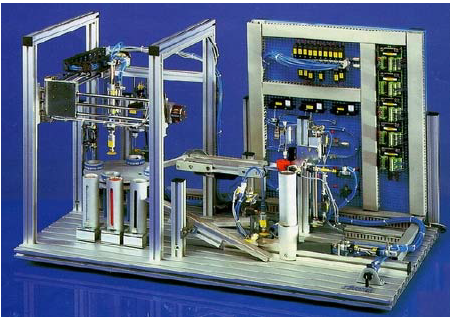
\includegraphics[scale=0.75]{FestoMPSSystem2.png}
					\caption{Το πλήρες σύστημα Festo MPS\textregistered}
					\label{φωτ:Το πλήρες σύστημα Festo MPS}
			\end{figure}
			
			\begin{figure}[hp]
					\centering
					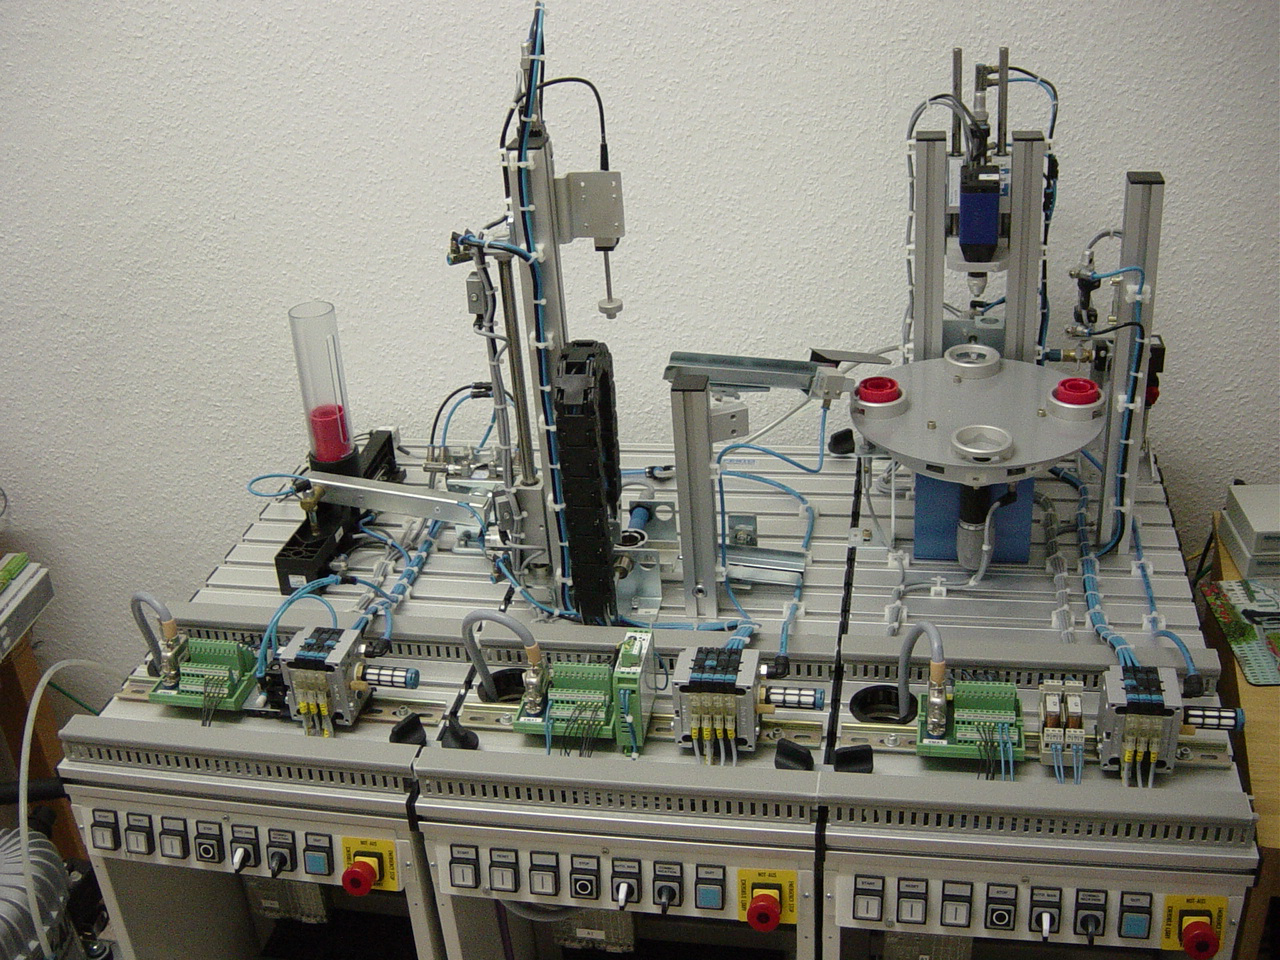
\includegraphics[scale=0.25]{FestoMPSSystem1.png}
					\caption{Το σύστημα Festo MPS\textregistered  χωρίς τον τελικό σταθμό αποθήκευσης \cite{PhotosFestoMPSUniversityHalle}}
					\label{φωτ:Το σύστημα Festo MPS χωρίς τον τελικό σταθμό αποθήκευσης}
			\end{figure}
			
			\paragraph{Κατασκευή} {Το σύστημα έχει κατασκευαστεί από την εταιρεία Festo Didactic\footnote{http://www.festo-didactic.com} \index{Festo Didactic}. Συγκεκριμένα η εταιρεία αυτή ειδικεύεται στη διδασκαλία συστημάτων αυτοματισμού. Για το σκοπό κατασκευάζει μικρογραφίες εξαρτημάτων όπως βαλβίδες πίεσης, κινητήρες, ρομποτικούς βραχίονες κ.ά. τα οποία συνδυαζώμενα μεταξύ τους αποδίδουν πληθώρα βιομηχανικών διεργασιών και συστημάτων παραγωγής. Ένα τέτοιο σύστημα αποτελεί και το συγκεκριμένο που θα αναλυθεί στη συνέχεια για τις ανάγκες της εργασίας.
			}
			
			\paragraph{Αιτιολόγηση επιλογής} {Επιλέξαμε το συγκεκριμένο σύστημα ως περίπτωση εφαρμογής για τη \acrshort{SysML} επειδή διαθέτει πολλά ενδιαφέροντα στοιχεία για έναν \glsuseriii{Μηχανικός συστημάτων} αφού αποτελείται από εξαρτήματα που ανήκουν σε διαφορετικά επιστημονικά πεδία. Συγκεκριμένα διαθέτει αισθητήρες που η αρχή λειτουργίας τους βασίζεται σε οπτική, επαγωγική, χωρητική και μηχανική μέτρηση. Επιπλέον περιλαμβάνει ηλεκτρικά, ηλεκτρονικά και μηχανικά μέρη, ρομποτικούς βραχίονες, βαλβίδες πίεσης, πνευματικές συσκευές κ.ά.. Μην ξεχνάμε ότι στο όλο σύστημα συμπεριλαμβάνεται και το λογισμικό ελέγχου της παραγωγικής διαδικασίας. Συνεπώς για την κατανόηση του απαιτούνται γνώσεις ηλεκτρολόγου, ηλεκτρονικού και μηχανολόγου μηχανικού καθώς και μηχανικού λογισμικού.
			}
						
			\paragraph{Πρώτες ύλες} {Ως πρώτες ύλες\index{πρώτη ύλη}\index{κυλινδρικά τεμάχια}\index{τεμάχια} χρησιμοποιούνται κυλινδρικά αντικείμενα διαφορετικού χρώματος, υλικού και ύψους. Μπορεί να είναι χρώματος κόκκινο, μαύρο ή ασημί και κατασκευασμένα από αλουμίνιο ή πλαστικό. Όσον αφορά το ύψος τους, τα κόκκινα και μεταλλικά τεμάχια είναι κατά 2,5 χιλιοστά ψηλότερα των αντίστοιχων μαύρων.
			}
			
			\begin{figure}[hp]
					\centering
					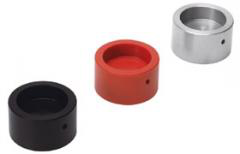
\includegraphics[scale=0.25]{WorkpiecesFesto.png}
					\caption{Οι πρώτες ύλες της γραμμής παραγωγής}
					\label{φωτ:Οι πρώτες ύλες της γραμμής παραγωγής}
			\end{figure}
		
			\paragraph{Παραγωγική διαδικασία} {Η παραγωγική διαδικασία που αναπαριστάμε έχει ως βάση της κυλινδρικά τεμάχια διάφορων χρωμάτων, υλικών και ύψους. Τα τεμάχια αυτά είναι αποθηκευμένα σε μία στοίβα στο σταθμό διανομής {\footnotesize (βλπ ενότ.~\ref{ενότ:Σταθμός διανομής})}. Με τη βοήθεια ενός βραχίονα μεταφέρονται στο σταθμό ελέγχου {\footnotesize (βλπ ενότ.~\ref{ενότ:Σταθμός ελέγχου})} όπου αναγνωρίζεται το χρώμα και το υλικό των κυλίνδρων και ελέγχονται για το ύψος τους. Αν κάποιος κύλινδρος διαθέτει μία ή και περισσότερες μη αποδεκτές ιδιότητες τότε απομακρύνεται από τη γραμμή παραγωγής. Οι αποδεκτοί πλέον κύλινδροι μεταβαίνουν στο σταθμό επεξεργασίας {\footnotesize (βλπ ενότ.~\ref{ενότ:Σταθμός επεξεργασίας})}. Στο σταθμό αυτό δημιουργείται μία οπή στο κέντρο των κυλίνδρων. Στη συνέχεια ελέγχεται αν η η διάτρηση ήταν επιτυχής και εν τέλει αποθηκεύονται στο σταθμό αποθήκευσης {\footnotesize (βλπ ενότ.~\ref{ενότ:Σταθμός αποθήκευσης})} σε μία από τρεις στοίβες ανάλογα με το χρώμα και το υλικό τους. \cite{UMLΕνσωματωμέναΣυστήματα}
			}
			
			\paragraph{} {Ακολουθεί η λειτουργική ανάλυση της κάθε μονάδας παραγωγής και η καταγραφή των επιμέρους μερών τους.}
			}

%%%%%%%%%%%%%%%%%%%%%%%%%%%%%%%%%%%%%%%%%%%%%%%%%%%%%%%%%%%%%
%%%%%%%%%%%%%%		   							Υποενότητα		   					   %%%%%%%%%%%%%%%%%%%%
			\FloatBarrier
			\subsection{Σταθμός διανομής \cite{FestoMPSDistributionStationManual} \cite{ΤοΦυσικόΣύστημαFestoMPS} \cite{UMLΕνσωματωμέναΣυστήματα}}
			
			\label{ενότ:Σταθμός διανομής}
				\paragraph{Εισαγωγή} {Ο σταθμός διανομής\index{σταθμός!διανομής} αναλαμβάνει την εισαγωγή των πρώτων υλών στη γραμμή παραγωγής από μία στοίβα αποθήκευσης\index{στοίβα αποθήκευσης} και τη διανομή τους με τη χρήση βραχίονα\index{βραχίονας} και βεντούζας\index{βεντούζα}. Αποτελείται από τα εξαρτήματα :
				}
				\begin{itemize}
					\item στοίβα αποθήκευσης {\footnotesize (βλπ. σχ.\ref{φωτ:Η στοίβα αποθήκευσης από Festo})}
					\item μονάδα μεταφοράς {\footnotesize (βλπ. σχ.\ref{φωτ:Η μονάδα μεταφοράς από Festo})}
					\item βάση εγκατάστασης
					\item συσκευή ελέγχου
					\item πλακέτα plc
				\end{itemize}
				\paragraph{} {Ο σταθμός διανομής διαχωρίζει τα κυλινδρικά τεμάχια από τη στοίβα αποθήκευσης η οποία διατηρεί μέχρι 8 κομμάτια. Το επίπεδο πλήρωσης της στοίβας ελέγχεται μέσω ενός \glsuseri{φωτοκύτταρο}. Οι κύλινδροι αφαιρούνται ένας-ένας από τη στοίβα μέσω ενός \glsuseri{έμβολο πεπιεσμένου αέρα δύο κατευθύνσεων}. Στη συνέχεια η \gls{μονάδα μεταφοράς} παραλαμβάνει τα τεμάχια και τα παραδίδει στον επόμενο σταθμό της γραμμής παραγωγής. Αυτό επιτυγχάνεται με τη χρήση ενός ρομποτικού βραχίονα και μιας \glsuseri{βεντούζα}. Η βεντούζα δεσμεύει το τεμάχιο με μία βαλβίδα κενού και ένας \gls{αισθητήρας κενού} ανιχνεύει τη δέσμευση του. Τότε ο βραχίονας μεταφοράς, οδηγούμενος από έναν κινητήρα περιστροφικής κίνησης, παραδίδει τον κύλινδρο στην επόμενη μονάδα.
				}
				
				\begin{figure}[hp]
					\centering
					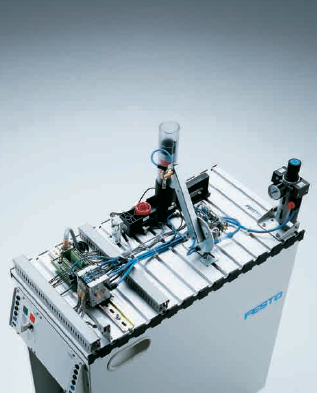
\includegraphics[scale=0.25]{DistributionStationFesto.png}
					\caption{Ο σταθμός διανομής \cite{OverviewMPSStations}}
					\label{φωτ:Ο σταθμός διανομής από Festo}
				\end{figure}
				
				\begin{figure}[hp]
					\centering
					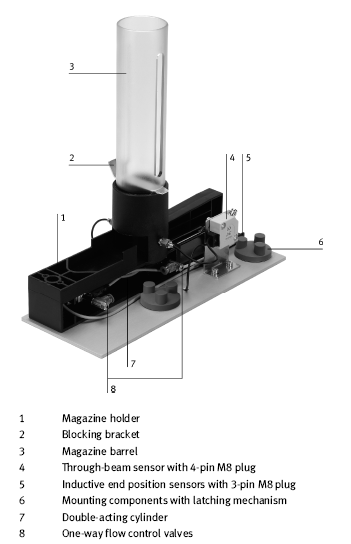
\includegraphics[scale=0.75]{StackModuleParts.png}
					\caption{Η στοίβα αποθήκευσης \cite{FestoStackMagazineModuleManual}}
					\label{φωτ:Η στοίβα αποθήκευσης από Festo}
				\end{figure}
				
				\begin{figure}[hp]
					\centering
					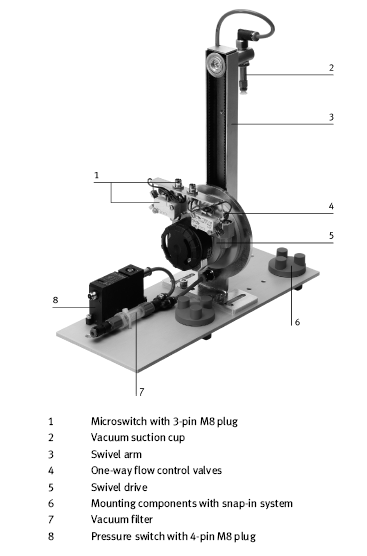
\includegraphics[scale=0.75]{ChangerModuleParts.png}
					\caption{Η μονάδα μεταφοράς \cite{FestoChangerModuleManual}}
					\label{φωτ:Η μονάδα μεταφοράς από Festo}
				\end{figure}
							

				
				\paragraph{Στοίβα αποθήκευσης {\footnotesize βλπ. σχ. \ref{φωτ:Η στοίβα αποθήκευσης από Θράμπο} και \ref{φωτ:Η στοίβα αποθήκευσης από Festo}}} {Όπως προαναφέρθηκε η στοίβα αποθήκευσης χωράει μέχρι 8 τεμάχια. Ένα πναυματικό έμβολο διπλής κατεύθυνσης μεταφέρει τα κομμάτια στην άκρη της μονάδας αυτής\index{έμβολο!διπλής κατεύθυνσης}. Τα τεμάχια σταματάνε στο σημείο αυτό επειδή υπάρχει κυκλικό τοιχίο που εμποδίζει οποιαδήποτε άλλη τοποθέτηση. Στη θέση αυτή χωράει μόνο ένα τεμάχιο και αποτελεί τη θέση από την οποία μεταφέρεται ο κύλινδρος στην επόμενη μονάδα.Το επόμενο τεμάχιο τοποθετείται αυτόματα μπροστά από το έμβολο με τη βοήθεια της βαρύτητας.
				}
				\paragraph{} {Η διαθεσιμότητα των τεμαχίων μέσα στη στοίβα διαπιστώνεται μέσω ενός φωτοκυττάρου\index{φωτοκύτταρο} τοποθετούμενο στο κάτω μέρος αυτής. Η θέση του εμβόλου διαπιστώνεται μαγνητικά μέσω δύο επαγωγικών αισθητήρων\index{επαγωγικός αισθητήρας}\index{αισθητήρας!επαγωγικός} -ο ένας αισθητήρας τοποθετείται στο πίσω μέρος και ο άλλος στο μπροστινό. Η ταχύτητα εκτόνωσης και επαναφοράς του εμβόλου καθορίζεται με μεγάλη ακρίβεια από \gls{βαλβίδα ελέγχου πεπιεσμένου αέρα μίας κατεύθυνσης}\index{βαλβίδα}.
				}

				\begin{figure}[hp]
					\centering
					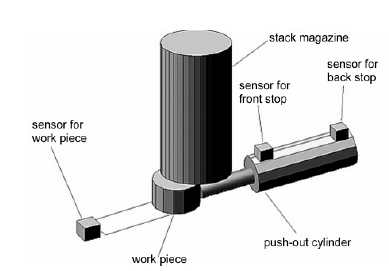
\includegraphics[scale=0.7]{StackModulePartsThrambo.png}
					\caption{Γραφική απεικόνιση της στοίβας αποθήκευσης \cite{ΤοΦυσικόΣύστημαFestoMPS}}
					\label{φωτ:Η στοίβα αποθήκευσης από Θράμπο}
				\end{figure}
	
				\paragraph{Μονάδα μεταφοράς {\footnotesize βλπ. σχ. \ref{φωτ:Η μονάδα μεταφοράς από Θράμπο} και \ref{φωτ:Η στοίβα αποθήκευσης από Festo}}} {\index{μονάδα!μεταφοράς}Η μονάδα αυτή αποτελεί μία πνευματική συσκευή. Μέσω μίας βεντούζας που είναι τοποθετημένη πάνω σε ρομποτικό βραχίονα τα τεμάχια μεταφέρονται με περιστροφική κίνηση\index{περιστροφική κίνηση} στην επόμενη μονάδα. Η περιστροφική κίνηση υλοποιείται από έναν πνευματικό κινητήρα\index{κινητήρας!πνευματικός}. Το εύρος της περιστροφικής κίνησης καθορίζεται μηχανικά μεταξύ 0 και 180 μοιρών. Οι τελικές θέσεις που λαμβάνει ο βραχίονας ελέγχονται μέσω \glsuserii{μικροδιακόπτης}\index{μικροδιακόπτης}. Τέλος μέσω ενός αισθητήρα κενού\index{αισθητήρας!κενού} συνδεδεμένο με τη βεντούζα ανιχνεύεται αν η τελευταία έχει παραλάβει το κυλινδρικό τεμάχιο.
				}
				\begin{figure}[hp]
					\centering
					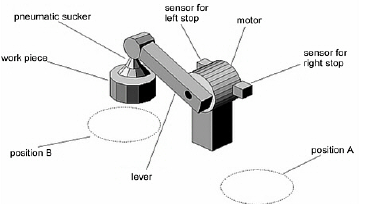
\includegraphics[scale=0.7]{ChangerModulePartsThrambo.png}
					\caption{Γραφική απεικόνιση της μονάδας μεταφοράς \cite{ΤοΦυσικόΣύστημαFestoMPS}}
					\label{φωτ:Η μονάδα μεταφοράς από Θράμπο}
				\end{figure}
				
				\paragraph{Ανάλυση λειτουργίας} {Λεπτομερέστερα οι προϋποθέσεις για να λειτουργήσει ο σταθμός αυτός και η σειρά με την οποία εκτελούνται οι επιμέρους ενέργειες απαριθμούνται στον πίνακα \ref{πιν.:Ανάλυση λειτουργίας του σταθμού διανομής}:
				}
				\begin{longtable} { m{0.5cm} m{12cm} }
					\caption [Ανάλυση λειτουργίας του σταθμού διανομής]  {Ανάλυση λειτουργίας του σταθμού διανομής \cite{FestoMPSDistributionStationManual}}
					\label{πιν.:Ανάλυση λειτουργίας του σταθμού διανομής}\\
					\hline
					\endfirsthead
					\multicolumn{2}{c}{συνέχεια του πίνακα \ref{πιν.:Ανάλυση λειτουργίας του σταθμού διανομής}}\\
					\hline
					~\\
					\endhead
					\hline
					\multicolumn{2}{c}{ο πίνακας συνεχίζεται στην επόμενη σελίδα}\\
					\endfoot
					\multicolumn{2}{c}{ολοκληρώθηκε ο πίνακας \ref{πιν.:Ανάλυση λειτουργίας του σταθμού διανομής}}\\
					\endlastfoot
					~\\
					\multicolumn{2}{c}{Προαπαιτήσεις}\\
					1 & Η στοίβα να διαθέτει τεμάχια προς επεξεργασία\\
					\hline
					~\\
					\multicolumn{2}{c}{Αρχική κατάσταση}\\
					1 & Το έμβολο διπλής κατεύθυνσης είναι σε κατάσταση εκτόνωσης\\
					2 & Το σύστημα βραχίονα-κινητήρα βρίσκεται στη μεριά της στοίβας\\
					3 & Η βεντούζα είναι ανενεργή\\
					\hline
					~\\
					\multicolumn{2}{c}{Ακολουθία ενεργειών}\\
					1 & Ο κινητήρας μεταβαίνει στη θέση του επόμενου σταθμού εάν υπάρχουν τεμάχια μέσα στη στοίβα και το πλήκτρο Εκκίνηση έχει πατηθεί\\
					2 & Το έμβολο επανέρχεται και βγάζει ένα τεμάχιο έξω από τη στοίβα\\
					3 & Ο κινητήρας μεταβαίνει στη θέση της στοίβας αποθήκευσης\\
					4 & Η βαλβίδα κενού ενεργοποιείται και μόλις πιαστεί το τεμάχιο ο διακόπτης κενού στέλνει το απαραίτητο σήμα\\
					5 & Το έμβολο επανέρχεται και ελευθερώνει το τεμάχιο\\
					6 & Ο κινητήρας μεταβαίνει στη θέση του επόμενου σταθμού\\
					7 & Η βαλβίδα κενού απενεργοποιείται\\
					8 & Ο κινητήρας μεταβαίνει στη θέση της στοίβας\\
					\hline
				\end{longtable}
			
%%%%%%%%%%%%%%%%%%%%%%%%%%%%%%%%%%%%%%%%%%%%%%%%%%%%%%%%%%%%%
%%%%%%%%%%%%%%		   							Υποενότητα		   					   %%%%%%%%%%%%%%%%%%%%
			\FloatBarrier
			\subsection{Σταθμός ελέγχου \cite{FestoMPSTestingStationManual} \cite{ΤοΦυσικόΣύστημαFestoMPS} \cite{UMLΕνσωματωμέναΣυστήματα}}
			
			\label{ενότ:Σταθμός ελέγχου}
				\paragraph{Εισαγωγή} {Ο σταθμός ελέγχου\index{σταθμός!ελέγχου} αναλαμβάνει να διαπιστώσει αν το τεμάχιο που παρέλαβε από το σταθμό διανομής {\footnotesize βλπ. ενοτ.\ref{ενότ:Σταθμός διανομής}} είναι κατάλληλο επεξεργασίας από τον επόμενο σταθμό -σταθμός επεξεργασίας {\footnotesize βλπ. ενοτ.\ref{ενότ:Σταθμός επεξεργασίας}}. Συγκεκριμένα πρέπει να αναγνωρίσει το υλικό κατασκευής των κυλίνδρων, να ελέγξει το ύψος των τεμαχίων και ανάλογα με αυτό να τον απορρίψει  ή να τον προωθήσει στον επόμενο σταθμό της γραμμής παραγωγής. Αποτελείται από τα εξαρτήματα :
				}
				\begin{itemize}
					\item μονάδα αναγνώρισης
					\item μονάδα ανύψωσης
					\item μονάδα μέτρησης
					\item μονάδα κύλισης με αέρα
					\item μονάδα κύλισης
					\item βάση εγκατάστασης
					\item συσκευή ελέγχου
					\item πλακέτα plc
				\end{itemize}
				\paragraph{} {Ο σταθμός ελέγχου εξακριβώνει τα χαρακτηριστικά των κυλινδρικών τεμαχίων. Η μονάδα αναγνώρισης διαπιστώνει το χρώμα του κυλίνδρου και την παρουσία τεμαχίου. Με \glsuseri{αισθητήρας ανάκλασης}\index{αισθητήρας!ανάκλασης} ελέγχουμε αν η θέση μέτρησης είναι διαθέσιμη ώστε να αποφασιστεί αν θα ανυψωθεί το κυλινδρικό αντικείμενο ή όχι. Επιπλέον, ένας \gls{αναλογικός αισθητήρας}\index{αισθητήρας!αναλογικός} μετράει το ύψος του κυλίνδρου. Το σήμα εξόδου του αισθητήρα μετατρέπεται σε ψηφιακό μέσω ενός τελεστή με ρυθμιζόμενο κατώφλι ή μπορεί να εισαχθεί σε ένα PLC ως αναλογικό σήμα. Τέλος αν οι κύλινδροι είναι αποδεκτοί οδηγούνται από το επίπεδο που είναι με ένα πνευματικό \gls{γραμμικό έμβολο}\index{έμβολο!γραμμικό} δύο κατευθύνσεων προς τον σταθμό επεξεργασίας διαμέσου μιας \glsuseri{πλατφόρμα κύλισης με εξομάλυνση αέρα}\index{πλατφόρμα κύλισης!εξομάλυνση αέρα}. Τα υπόλοιπα κομμάτια "κατεβαίνουν" πίσω με τον ανελκυστήρα και τοποθετούνται σε μία διπλανή \gls{πλατφόρμα κύλισης}.
				}
				
				\begin{figure}[hp]
					\centering
					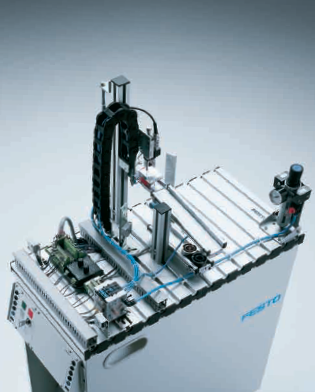
\includegraphics[scale=0.25]{TestingStationFesto.png}
					\caption{Ο σταθμός ελέγχου \cite{OverviewMPSStations}}
					\label{φωτ:Ο σταθμός ελέγχου από Festo}
				\end{figure}
								
				\paragraph{Μονάδα αναγνώρισης {\footnotesize βλπ. σχ. \ref{φωτ:Η μονάδα αναγνώρισης από Festo}}\index{μονάδα!αναγνώρισης}} {Η μονάδα αυτή αποτελείται από 2 \glsplural{αισθητήρας προσέγγισης}\index{αισθητήρας!προσέγγισης} με ψηφιακή έξοδο, έναν χωρητικό και έναν οπτικό\index{αισθητήρας!οπτικός}. Ο χωρητικός ανιχνεύει την παρουσία τεμαχίου ανεξαρτήτως χρώματος. Αντίστοιχα ο οπτικός αισθητήρας διάχυσης ανιχνεύει το χρώμα των αντικειμένων. Επειδή η αρχή λειτουργίας του βασίζεται στην ποσότητα του επιστρεφόμενου φωτός, δεν μπορούν να ανιχνευθούν τα μαύρα τεμάχια. Ο οπτικός αισθητήρας τοποθετείται πάνω στην πλατφόρμα ανύψωσης.
				}
				\begin{figure}[hp]
					\centering
					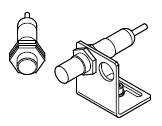
\includegraphics[scale=1]{TestingStationRecognitionModule.png}
					\caption{Η μονάδα αναγνώρισης \cite{FestoMPSTestingStationManual}}
					\label{φωτ:Η μονάδα αναγνώρισης από Festo}
				\end{figure}
				
				\paragraph{Μονάδα ανύψωσης {\footnotesize βλπ. σχ. \ref{φωτ:Η μονάδα ανύψωσης από Festo}}\index{μονάδα!ανύψωσης}} {Η ανύψωση πραγματοποιείται με ένα \gls{πνευματικό έμβολο}\index{έμβολο!πνευματικό} δύο κατευθύνσεων. Η χαμηλή και ψηλή θέση του εντοπίζονται μέσω \glsuserii{μαγνητικός αισθητήρας}\index{αισθητήρας!μαγνητικός} ή \glsuserii{επαγωγικός αισθητήρας}\index{αισθητήρας!επαγωγικός}. Επιπλέον, διαθέτει ένα πνευματικό \gls{έμβολο εκτίναξης}\index{έμβολο!εκτίναξης} δύο κατευθύνσεων για την απομάκρυνση των αποδεκτών τεμαχίων στην μονάδα κύλισης με εξομάλυνση αέρα και των απορριφθέντων τεμαχίων στην απλή μονάδα κύλισης. Η θέση του εμβόλου αυτού διαπιστώνεται μέσω δύο μαγνητικών αισθητήρων, έναν στο μπροστινό τμήμα του και ένα στο πίσω. Τέλος, για την καλύτερη και ασφαλέστερη εγκατάσταση των εξαρτημάτων αυτών χρησιμοποιείται και ένας οδηγός τύπου αλυσίδας για ενθυλακώσει τα ηλεκτρικά καλώδια και τους σωλήνες μεταφοράς πεπιεσμένου αέρα της διάταξης. Επισημαίνουμε ότι ο οπτικός αισθητήρας της μονάδας αναγνώρισης ενσωματώνεται πάνω στην πλατφόρμα ανύψωσης.
				}
				\begin{figure}[hp]
					\centering
					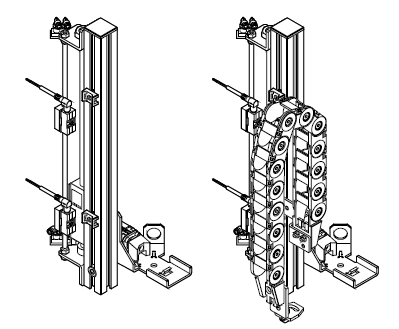
\includegraphics[scale=0.5]{TestingStationLiftingModule.png}
					\caption{Η μονάδα ανύψωσης \cite{FestoMPSTestingStationManual} (στη δεύτερη εικόνα εμφανίζεται ο οδηγός καλωδίων στον οποίο τοποθετούνται τα ηλεκτρικά καλώδια και οι σωλήνες μεταφοράς πεπιεσμένου αέρα)}
					\label{φωτ:Η μονάδα ανύψωσης από Festo}
				\end{figure}
				
				\paragraph{Μονάδα μέτρησης {\footnotesize βλπ. σχ. \ref{φωτ:Η μονάδα μέτρησης από Festo} και \ref{φωτ:Σχηματική απεικόνιση της μονάδας μέτρησης από Θράμπο}}\index{μονάδα!μέτρησης}} {Αποτελείται από ένα αναλογικό αισθητήρα για τη μέτρηση του ύψους των τεμαχίων. Η αρχή λειτουργίας βασίζεται σε έναν γραμμικό ποτενσιόμετρο και ένα διαιρέτη τάσης. Η αναλογική μέτρηση μπορεί να μετατραπεί σε ψηφιακή μέσω ενός τελεστή ή να τροφοδοτηθεί σε μία plc συσκευή. Τέλος υπάρχει αποσβέστης ταλαντώσεων που δημιουργούνται από την ανύψωση του αντικειμένου στην τελική του θέση.\\Επισημαίνουμε ότι τα κόκκινα και μεταλλικά τεμάχια είναι κατά 2,5 χιλιοστά ψηλότερα των αντίστοιχων μαύρων.
				}
				\begin{figure}[hp]
					\centering
					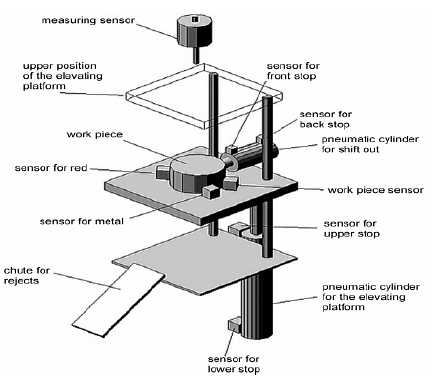
\includegraphics[scale=1]{TestingStationPartsThrambo.png}
					\caption{Σχηματική απεικόνιση της μονάδας μέτρησης \cite{ΤοΦυσικόΣύστημαFestoMPS}}
					\label{φωτ:Σχηματική απεικόνιση της μονάδας μέτρησης από Θράμπο}
				\end{figure}	
				
				\begin{figure}[hp]
					\centering
					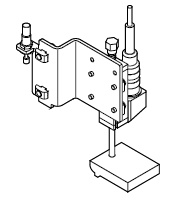
\includegraphics[scale=1]{TestingStationMeasuringModule.png}
					\caption{Η μονάδα μέτρησης \cite{FestoMPSTestingStationManual}}
					\label{φωτ:Η μονάδα μέτρησης από Festo}
				\end{figure}			
				
				\paragraph{Μονάδα κύλισης με εξομάλυνση αέρα {\footnotesize βλπ. σχ. \ref{φωτ:Η μονάδα κύλισης με εξομάλυνση αέρα από Festo} και \ref{φωτ:Σχηματική απεικόνιση της μονάδας κύλισης με εξομάλυνση αέρα από Θράμπο}}\index{μονάδα!κύλισης με εξομάλυνση αέρα}} {Η μονάδα κύλισης με εξομάλυνση αέρα χρησιμοποιείται για τη μεταφορά των κυλίνδρων με μέγιστη χωρητικότητα πέντε (5). Η εξομάλυνση από τον αέρα μειώνει την τριβή μεταξύ των τεμαχίων και της πλατφόρμας. Η γωνία κλίσης της πλατφόρμας είναι ρυθμιζόμενη. Στο τέλος της πλατφόρμας δεν υπάρχει τοιχίο για να εμποδίζει την κύλιση των κυλίνδρων. Επιθυμούμε την απρόσκοπτη κύλιση τους στον επόμενο σταθμό.
				}
				\begin{figure}[hp]
					\centering
					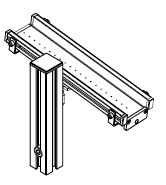
\includegraphics[scale=1]{TestingStationAirCushionedSlideModule.png}
					\caption{Η μονάδα κύλισης με εξομάλυνση αέρα \cite{FestoMPSTestingStationManual}}
					\label{φωτ:Η μονάδα κύλισης με εξομάλυνση αέρα από Festo}
				\end{figure}
				\begin{figure}[hp]
					\centering
					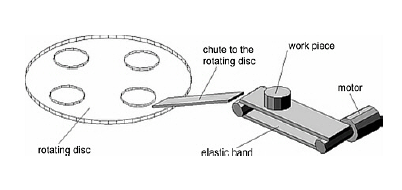
\includegraphics[scale=1]{TestingStationAirCushionedSlideTrambo.png}
					\caption{Σχηματική απεικόνιση της μονάδας κύλισης με εξομάλυνση αέρα \cite{ΤοΦυσικόΣύστημαFestoMPS}}
					\label{φωτ:Σχηματική απεικόνιση της μονάδας κύλισης με εξομάλυνση αέρα από Θράμπο}
				\end{figure}
				
				\paragraph{Μονάδα κύλισης {\footnotesize βλπ. σχ. \ref{φωτ:Η μονάδα κύλισης από Festo}} \index{μονάδα!κύλισης}} {Η μονάδα κύλισης χρησιμοποιείται για τη μεταφορά των κυλίνδρων. Τέσσερα (4) στο σύνολο μπορούν να τοποθετηθούν στην πλατφόρμα. Η γωνία κλίσης είναι ρυθμιζόμενη.
				}
				\begin{figure}[hp]
					\centering
					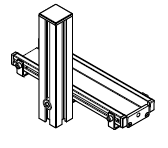
\includegraphics[scale=1]{TestingStationSlideModule.png}
					\caption{Η μονάδα κύλισης \cite{FestoMPSTestingStationManual}}
					\label{φωτ:Η μονάδα κύλισης από Festo}
				\end{figure}
				
				
				\paragraph{Ανάλυση λειτουργίας} {Λεπτομερέστερα οι προϋποθέσεις για να λειτουργήσει ο σταθμός αυτός και η σειρά με την οποία εκτελούνται οι επιμέρους ενέργειες απαριθμούνται στον πίνακα \ref{πιν.:Ανάλυση λειτουργίας του σταθμού ελέγχου}:
				}
				\begin{longtable} { m{0.5cm} m{12cm} }
					\caption [Ανάλυση λειτουργίας του σταθμού ελέγχου]  {Ανάλυση λειτουργίας του σταθμού ελέγχου \cite{FestoMPSTestingStationManual}}
					\label{πιν.:Ανάλυση λειτουργίας του σταθμού ελέγχου}\\
					\hline
					\endfirsthead
					\multicolumn{2}{c}{συνέχεια του πίνακα \ref{πιν.:Ανάλυση λειτουργίας του σταθμού ελέγχου}}\\
					\hline
					~\\
					\endhead
					\hline
					\multicolumn{2}{c}{ο πίνακας συνεχίζεται στην επόμενη σελίδα}\\
					\endfoot
					\multicolumn{2}{c}{ολοκληρώθηκε ο πίνακας \ref{πιν.:Ανάλυση λειτουργίας του σταθμού ελέγχου}}\\
					\endlastfoot
					~\\
					\multicolumn{2}{c}{Προαπαιτήσεις}\\
					1 & Ένα τεμάχιο βρίσκεται έτοιμο για παραλαβή στο σταθμό διανομής\\
					2 & Κανένα άλλο τεμάχιο δεν καταλαμβάνει την θέση αναγνώρισης\\
					\hline
					~\\
					\multicolumn{2}{c}{Αρχική κατάσταση}\\
					1 & Ο ανελκυστήρας μεταβαίνει στην χαμηλή θέση\\
					2 & Το έμβολο εκτίναξης συμπτύσσεται\\
					3 & Απενεργοποίηση της πλατφόρμας κύλισης με εξομάλυνση αέρα\\
					\hline
					~\\
					\multicolumn{2}{c}{Ακολουθία ενεργειών}\\
					1 & Αναγνώριση χρώματος και υλικού των τεμαχίων\\
					2 & Ο ανελκυστήρας ανέρχεται στην πάνω θέση\\
					3 & Γίνεται έλεγχος του ύψους\\
					   & Αποδεκτό κυλινδρικό τεμάχιο\\
					 4 & Ενεργοποίηση της πλατφόρμας κύλισης με εξομάλυνση αέρα\\
					 5 & Έκταση του εμβόλου εκτίναξης\\
					 6 & Σύμπτυξη του εμβόλου εκτίναξης\\
					 7 & Απενεργοποίηση της πλατφόρμας κύλισης με εξομάλυνση αέρα\\
					 8 & Ο ανελκυστήρας κατέρχεται στην χαμηλή θέση\\
					 9 & Αρχική θέση\\
					  & Μη αποδεκτό κυλινδρικό τεμάχιο\\
					 10 & Ο ανελκυστήρας κατέρχεται στην χαμηλή θέση\\
					 11 & Έκταση του εμβόλου εκτίναξης\\
					 12 & Σύμπτυξη του εμβόλου εκτίναξης\\
					 13 & Αρχική θέση\\
					\hline
				\end{longtable}
				
				
%%%%%%%%%%%%%%%%%%%%%%%%%%%%%%%%%%%%%%%%%%%%%%%%%%%%%%%%%%%%%
%%%%%%%%%%%%%%		   							Υποενότητα		   					   %%%%%%%%%%%%%%%%%%%%			
			\FloatBarrier
			\subsection{Σταθμός επεξεργασίας \cite{FestoMPSProcessingStationManual} \cite{ΤοΦυσικόΣύστημαFestoMPS} \cite{UMLΕνσωματωμέναΣυστήματα}}
			
			\label{ενότ:Σταθμός επεξεργασίας}
				\paragraph{Εισαγωγή} {Ο σταθμός επεξεργασίας\index{σταθμός!επεξεργασίας} αναλαμβάνει να επεξεργαστεί τα κυλινδρικά τεμάχια. Συγκεκριμένα πρέπει να τους επιφέρει μία οπή στο πάνω μέρος τους. Αποτελείται από τα εξαρτήματα :
				}
				\begin{itemize}
					\item μονάδα περιστροφής
					\item μονάδα διάτρησης
					\item μονάδα ελέγχου
					\item βάση εγκατάστασης
					\item συσκευή ελέγχου
					\item πλακέτα plc
				\end{itemize}
				\paragraph{} {Ο σταθμός αυτός διαθέτει ένα περιστρεφόμενο δίσκο με τέσσερις (4) θέσεις για τα κυλινδρικά τεμάχια. Η θέση του δίσκου διαπιστώνεται με έναν επαγωγικό αισθητήρα, ο οποίος ανιχνεύει μεταλλική βίδα που υπάρχει σε κάθε μία από τις τέσσερις θέσεις. Αρχικά εισέρχεται κύλινδρος προς επεξεργασία. Ο δίσκος περιστρέφεται κατά $90^{\circ}$ στη θέση όπου βρίσκεται το τρυπάνι. Στη θέση αυτή το τεμάχιο ακινητοποιείται με τη βοήθεια ενός ηλεκτρομαγνητικού εμβόλου δύο κατευθύνσεων. Στη συνέχεια το τρυπάνι επιφέρει μία οπή στο τεμάχιο. Έπειτα ο δίσκος περιστρέφεται άλλες $90^{\circ}$. Στη θέση αυτή ελέγχεται αν η οπή είναι αποδεκτή. Ο έλεγχος γίνεται με μία ακίδα η οποία κινείται με μία ηλεκτρομαγνητική διάταξη. Τέλος, ο δίσκος περιστρέφεται κατά $90^{\circ}$ αναμένοντας το σταθμό αποθήκευσης να παραλάβει το επεξεργασμένο πλέον τεμάχιο.
				}
				\paragraph{} {Οι δύο διεργασίες του σταθμού αυτού -η διάτρηση και ο έλεγχος της οπής- γίνονται παράλληλα. Στον περιστερφόμενο δίσκο δεν εισέρχεται ένα τεμάχιο, επεξεργάζεται, ελέγχεται και μεταβαίνει στη μονάδα αποθήκευσης και έπειτα ένα δεύτερο. Αντίθετα, μπορεί και οι τέσσερις θέσεις να είναι κατειλημμένες ταυτόχρονα από κυλινδρικά τεμάχια. Φυσικά κάθε τεμάχιο θα συμμετέχει και σε διαφορετική διεργασία.
				}
				\begin{figure}[hp]
					\centering
					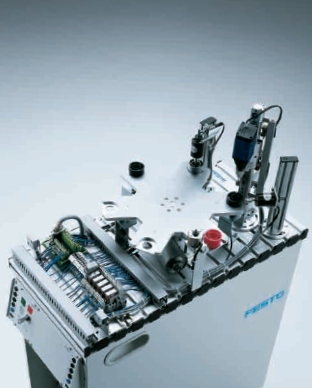
\includegraphics[scale=0.25]{ProcessingStationFesto.png}
					\caption{Ο σταθμός επεξεργασίας \cite{OverviewMPSStations}}
					\label{φωτ:Ο σταθμός επεξεργασίας από Festo}
				\end{figure}
								
				\paragraph{Μονάδα περιστροφής\index{μονάδα!περιστροφής}} {Η μονάδα αυτή ελέγχεται από μία \gls{μηχανή γραναζωτής σύμπλεξης συνεχούς ρεύματος}\index{μηχανή!συνεχούς ρεύματος}. Διαθέτει τέσσερις (4) θέσεις για να τις καταλάβουν τα τεμάχια. Σε κάθε θέση υπάρχει ένας χωρητικός αισθητήρας προσέγγισης για να διευκρινίζεται αν η θέση είναι πλήροις ή όχι.
				}
				
				\paragraph{Μονάδα διάτρησης {\footnotesize (βλπ. σχ. \ref{φωτ:Η μονάδα διάτρησης από Festo} και \ref{φωτ:Σχηματική αναπαράσταση της μονάδας διάτρησης από Θράμπο})}\index{μονάδα!διάτρησης}} {Στη θέση αυτή όταν διαπιστωθεί η ύπαρξη τεμαχίου ενεργοποιείται ένα πνευματικό έμβολο\index{έμβολο!ηλεκτρικό} δύο κατευθύνσεων για να το συγκρατήσει ακίνητο. Για τη καταγραφή της θέσης του εμβόλουχρησιμοποιούνται και πάλι δύο μαγνητικοί αισθητήρες, ένας μπροστά και ο δεύτερος στο πίσω μέρος. Στη συνέχεια το τρυπάνι\index{τρυπάνι} τρυπάει το τεμάχιο αυτό. Το τρυπάνι κινείται με τη βοήθεια ενός κινητήρα και η σύμπλεξη κινητήρα-τρυπανιού γίνεται μέσω οδοντωτού ιμάντα\index{οδοντωτός ιμάντας}\index{ιμάντας}. Η θέση του τρυπανιού ρυθμίζεται από δύο (2) ηλεκτρικούς τερματικούς διακόπτες\index{διακόπτης!ηλεκτρικός}\index{διακόπτης!τερματικός} που βρίσκονται στις δύο ακραίες θέσεις του τρυπανιού. Κάθε φορά που το σώμα από το τρυπάνι πλησιάζει έναν από τους δύο τερματικούς διακόπτες η κίνησή του αντιστρέφεται. Δηλαδή άμα κατέρχεται αλλάζει φορά και ανέρχεται και αντίστροφα. Υπενθυμίζεται ότι στη θέση αυτή υπάρχει χωρητικός αισθητήρας για να εξακριβωθεί ότι η θέση είναι κατειλημμένη.
				}
				\begin{figure}[hp]
					\centering
					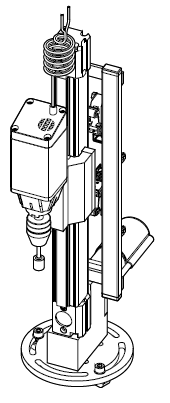
\includegraphics[scale=1]{ProcessingStationDrillingModuleFesto.png}
					\caption{Η μονάδα διάτρησης \cite{FestoMPSProcessingStationManual}}
					\label{φωτ:Η μονάδα διάτρησης από Festo}
				\end{figure}
				
				\begin{figure}[hp]
					\centering
					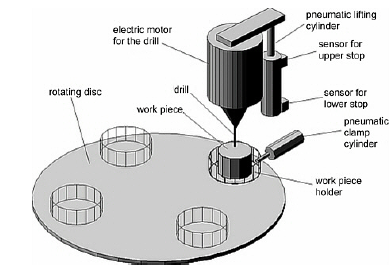
\includegraphics[scale=0.75]{ProcessingStationDrillingModuleThrambo.png}
					\caption{Σχηματική αναπαράσταση της μονάδας διάτρησης \cite{ΤοΦυσικόΣύστημαFestoMPS} {\footnotesize Παρατηρείται ότι το τρυπάνι κινείται με τη βοήθεια πνευματικού κυλίνδρου και όχι με ηλεκτρικό κινητήρα όπως αναφέρεται στο κείμενο. Καταγράψαμε την διάταξη όπως αυτή τεκμηριώνεται στο \cite{FestoMPSProcessingStationManual}. Η εικόνα παρατίθεται μόνο για να βοηθήσει να οπτικοποιηθεί το εν λόγω σύστημα}}
					\label{φωτ:Σχηματική αναπαράσταση της μονάδας διάτρησης από Θράμπο}
				\end{figure}
				
				\paragraph{Μονάδα ελέγχου {\footnotesize (βλπ. σχ. \ref{φωτ:Η μονάδα ελέγχου από Festo} και \ref{φωτ:Σχηματική αναπαράσταση της μονάδας ελέγχου από Θράμπο})}\index{μονάδα!ελέγχου}} {Η μονάδα ελέγχου αποτελεί μία \gls{ηλεκτρομαγνητική διάταξη}\index{ηλεκτρομαγνητική διάταξη}. Υπάρχει ένα πηνίο το οποίο παραμένει πακτωμένο στο πάνω μέρος του κορμού στήριξης. Όταν το πηνίο διαρρέεται από ρεύμα τότε, ο οπλισμός κατέρχεται και συνεπώς η ακίδα ελέγχου προσεγγίζει το επίπεδο του περιστρεφόμενου δίσκου, το επίπεδο δηλαδή του προς εξέταση κυλίνδρου. Για την διαπίστωση της θέσης του συστήματος ακίδας-οπλισμού χρησιμοποιούνται δύο επαγωγικοί αισθητήρες προσέγγισης\index{αισθητήρας!επαγωγικός}\index{αισθητήρας!προσέγγισης} οι οποίοι ενεργοποιούνται μέσω ενός μεταλλικού παξιμαδιού βρισκόμενο στο πάνω μέρος του συστήματος ακίδας-οπλισμού. Για τη διαπίστωση της ορθότηταας της τρύπας, η ακίδα της διάταξης αποτελεί ένα επαγωγικός αισθητήρας προσέγγισης.  Υπενθυμίζεται ότι στη θέση αυτή υπάρχει χωρητικός αισθητήρας για να εξακριβωθεί ότι η θέση είναι κατειλημμένη.
				}
				\begin{figure}[hp]
					\centering
					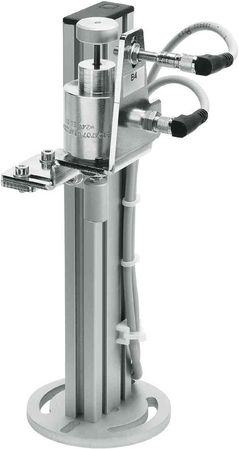
\includegraphics[scale=0.5]{ProcessingStationTestingModuleFesto.png}
					\caption{Η μονάδα ελέγχου {\footnotesize http://www.festo-didactic.com/int-en/learning-systems/mps-the-modular-production-system/project-kits/components-modules/testing-module.htm?fbid=aW50LmVuLjU1Ny4xNy4xOC43MTAuMzk0MQ}}
					\label{φωτ:Η μονάδα ελέγχου από Festo}
				\end{figure}
				
				\begin{figure}[hp]
					\centering
					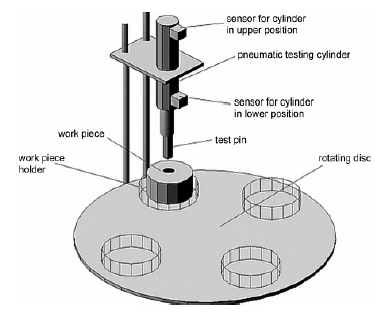
\includegraphics[scale=0.75]{ProcessingStationTestingModuleTrambo.png}
					\caption{Σχηματική αναπαράσταση της μονάδας ελέγχου \cite{ΤοΦυσικόΣύστημαFestoMPS} {\footnotesize Παρατηρείται ότι η ακίδα κινείται με τη βοήθεια πνευματικού κυλίνδρου και όχι με ηλεκτρομαγνητική διάταξη όπως αναφέρεται στο κείμενο. Καταγράψαμε την διάταξη όπως αυτή τεκμηριώνεται στο \cite{FestoMPSProcessingStationManual}. Η εικόνα παρατίθεται μόνο για να βοηθήσει να οπτικοποιηθεί το εν λόγω σύστημα}}
					\label{φωτ:Σχηματική αναπαράσταση της μονάδας ελέγχου από Θράμπο}
				\end{figure}			
				
				\paragraph{Ανάλυση λειτουργίας} {Λεπτομερέστερα οι προϋποθέσεις για να λειτουργήσει ο σταθμός αυτός και η σειρά με την οποία εκτελούνται οι επιμέρους ενέργειες απαριθμούνται στον πίνακα \ref{πιν.:Ανάλυση λειτουργίας του σταθμού επεξεργασίας}:
				}
				\begin{longtable} { m{0.5cm} m{12cm} }
					\caption [Ανάλυση λειτουργίας του σταθμού επεξεργασίας]  {Ανάλυση λειτουργίας του σταθμού επεξεργασίας \cite{FestoMPSProcessingStationManual}}
					\label{πιν.:Ανάλυση λειτουργίας του σταθμού επεξεργασίας}\\
					\hline
					\endfirsthead
					\multicolumn{2}{c}{συνέχεια του πίνακα \ref{πιν.:Ανάλυση λειτουργίας του σταθμού επεξεργασίας}}\\
					\hline
					\endhead
					\hline
					\multicolumn{2}{c}{ο πίνακας συνεχίζεται στην επόμενη σελίδα}\\
					\endfoot
					\multicolumn{2}{c}{ολοκληρώθηκε ο πίνακας \ref{πιν.:Ανάλυση λειτουργίας του σταθμού επεξεργασίας}}\\
					\endlastfoot
					~\\
					\multicolumn{2}{c}{Προαπαιτήσεις}\\
					1 & Κυλινδρικό τεμάχιο υπάρχει στην θέση υποδοχής του περιστρεφόμενου δίσκου\\
					\hline
					~\\
					\multicolumn{2}{c}{Αρχική κατάσταση}\\
					1 & Διαπιστώνεται η θέση του δίσκου\\
					2 & Η ακίδα ελέγχου βρίσκεται στην υψηλότερη θέση.\\
					3 & Το τρυπάνι διάτρησης βρίσκεται στην υψηλότερη θέση.\\
					4 & Το τρυπάνι είναι απενεργοποιημένο.\\
					5 & Το έμβολο συγκράτησης των κυλίνδρων στη θέση διάτρησης είναι σε κατάσταση σύμπτυξης.\\
					\hline
					~\\
					\multicolumn{2}{c}{Ακολουθία ενεργειών}\\
					  & Η ακολουθία αυτή αναφέρεται στην περίπτωση που ένα μόνο τεμάχιο βρίσκεται σε όλο τον περιστρεφόμενο δίσκο.\\
					1 & Ο δίσκος περιστρέφεται κατά $90^{\circ}$ εάν ανιχνευθεί τεμάχιο στη θέση υποδοχής. και το πλήκτρο εκκίνησης έχει πατηθεί.\\
					2 & Το έμβολο συγκράτησης εκτείνεται αφού πλέον το τεμάχιο βρίσκεται στη θέση διάτρησης. Το τρυπάνι ενεργοποιείται και κατέρχεται.\\
					3 & Μόλις το τρυπάνι φτάσει την κατώτατη θέση του, αυτόματα επανέρχεται στην ανώτερή του θέση.\\
					4 & Το τρυπάνι απενεργοποιείται και το έμβολο συγκράτησης συμπτύσεται.\\
					5 & Ο δίσκος περιστρέφεται κατά $90^{\circ}$.\\
					6 & Η ακίδα ελέγχου κατέρχεται και ελέγχει αν η οπή είναι η επιθυμητή.\\
					7 & Ο δίσκος περιστρέφεται κατά $90^{\circ}$ με αποτέλεσμα το τεμάχιο να μεταβεί στη θέση παραλαβής του από τον επόμενο σταθμό.\\
					\hline
				\end{longtable}

%%%%%%%%%%%%%%%%%%%%%%%%%%%%%%%%%%%%%%%%%%%%%%%%%%%%%%%%%%%%%
%%%%%%%%%%%%%%		   							Υποενότητα		   					   %%%%%%%%%%%%%%%%%%%%			
			\FloatBarrier
			\subsection{Σταθμός αποθήκευσης \cite{FestoMPSHandlingStationManual} \cite{ΤοΦυσικόΣύστημαFestoMPS} \cite{UMLΕνσωματωμέναΣυστήματα}}
			
			\label{ενότ:Σταθμός αποθήκευσης}
				\paragraph{Εισαγωγή} {Ο σταθμός αποθήκευσης\index{σταθμός!αποθήκευσης} αναλαμβάνει να μεταφέρει τα κυλινδρικά τεμάχια από τον περιστρεφόμενο δίσκο στις στοίβες αποθήκευσης. Αποτελείται από τα εξαρτήματα :
				}
				\begin{itemize}
					\item μονάδα μεταφοράς
					\item μονάδα αποθήκευσης
					\item βάση εγκατάστασης
					\item συσκευή ελέγχου
					\item πλακέτα plc
				\end{itemize}
				\paragraph{} {Το κυλινδρικό τεμάχιο το οποίο είναι έτοιμο για αποθήκευση παραλαμβάνεται από μία δαγκάνα με πνευματική αρχή λειτουργίας που κινείται με ένα σύστημα μεταφοράς δύο αξόνων. Ανάλογα με το είδος του κυλίνδρου και το γεγονός ότι η διάτρηση ήταν επιτυχής ή όχι, οι κύλινδροι μεταφέρονται σε τρεις (3) στοίβες. Αν το τεμάχιο είναι μαύρο τότε αποθηκεύεται στην πρώτη (εσωτερική) στοίβα. Αν το αντικείμενο είναι κόκκινου ή ασημί χρώματος τότε εναποτίθεται στην δεύτερη (μεσαία) στοίβα. Τέλος, αν η οπή δεν ειναι η επιθυμητή τότε μεταφέρεται στην τρίκη (εξωτερική) στοίβα.
				}
				\begin{figure}[hp]
					\centering
					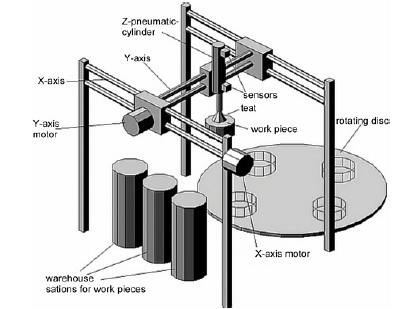
\includegraphics[scale=0.75]{HandlingStationTrambo.png}
					\caption{Ο σταθμός αποθήκευσης \cite{ΤοΦυσικόΣύστημαFestoMPS}  {\footnotesize Παρατηρείται ότι η διάταξη μεταφοράς περιλαμβάνει βεντούζα και όχι δαγκάνα όπως αναφέρεται στο κείμενο. Καταγράψαμε την διάταξη ως συνδυασμό των \cite{FestoMPSHandlingStationManual} και \cite{ΤοΦυσικόΣύστημαFestoMPS} με σκοπό την χρησιμοποίηση εξαρτημάτων από ποικίλα επιστημονικά πεδία. Η εικόνα παρατίθεται μόνο για να βοηθήσει να οπτικοποιηθεί το εν λόγω σύστημα}}
					\label{φωτ:Ο σταθμός αποθήκευσης από Θραμπο}
				\end{figure}
				
				\begin{figure}[hp]
					\centering
					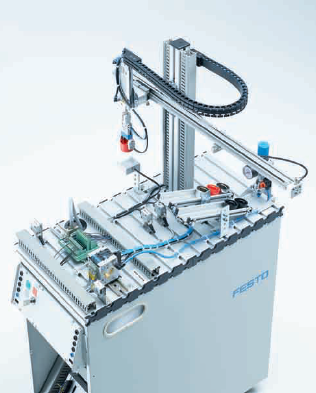
\includegraphics[scale=0.25]{HandlingStationFesto.png}
					\caption{Ο σταθμός αποθήκευσης \cite{OverviewMPSStations} {\footnotesize Παρατηρείται ότι η διάταξη μεταφοράς κινείται σε έναν άξονα μόνο και αντί για στοίβες διαθέτει πλατφόρμες κύλισης σε αντίθεση με το κείμενο. Καταγράψαμε την διάταξη ως συνδυασμό των \cite{FestoMPSHandlingStationManual} και \cite{ΤοΦυσικόΣύστημαFestoMPS} με σκοπό την χρησιμοποίηση εξαρτημάτων από ποικίλα επιστημονικά πεδία. Η εικόνα παρατίθεται μόνο για να βοηθήσει να οπτικοποιηθεί το εν λόγω σύστημα}}
					\label{φωτ:Ο σταθμός αποθήκευσης από Festo}
				\end{figure}
				
				\paragraph{Μονάδα μεταφοράς\index{μονάδα!μεταφοράς}} {Η μονάδα αυτή αποτελείται από ένα σύστημα μετακίνησης σε τρεις άξονες. Η μετακίνηση στο οριζόντιο επίπεδο επιτυγχάνεται με ηλεκτρικούς κινητήρες συνεχούς ρεύματος.Για την μετακίνηση στον κάθετο άξονα χρησιμοποιείται ένα πνευματικό έμβολο\index{έμβολο!πνευματικό} δύο κατευθύνσεων το οποίο διαθέτει μία δαγκάνα\index{δαγκάνα!πνευματική} στο άκρο του. Το έμβολο αυτό διαθέτει δύο μαγνητικούς αισθητήρες για την διαπίστωση των ακραίων θέσεων του. Η δαγκάνα κλείνει και ανοίγει με πεπιεσμένο αέρα διαθέτοντας επιπλέον και ένα οπτικό αισθητήρα ενσωματωμένο στο σώμα της για να ανιχνεύεται το κυλινδρικό τεμάχιο και το χρώμα αυτού.
				}
				
				\paragraph{Μονάδα αποθήκευσης\index{μονάδα!αποθήκευσης}} {Η μονάδα αυτή αποτελείται απλούστατα από τρεις (3) στοίβες όπως φαίνονται και στην εικόνα \ref{φωτ:Ο σταθμός αποθήκευσης από Θραμπο} χωρητικότητας οχτώ (8) τεμαχίων η καθεμία.
				}
				
				\paragraph{Ανάλυση λειτουργίας} {Λεπτομερέστερα οι προϋποθέσεις για να λειτουργήσει ο σταθμός αυτός και η σειρά με την οποία εκτελούνται οι επιμέρους ενέργειες απαριθμούνται στον πίνακα \ref{πιν.:Ανάλυση λειτουργίας του σταθμού αποθήκευσης}:
				}
				\begin{longtable} { m{0.5cm} m{12cm} }
					\caption [Ανάλυση λειτουργίας του σταθμού αποθήκευσης]  {Ανάλυση λειτουργίας του σταθμού αποθήκευσης \cite{FestoMPSHandlingStationManual}}
					\label{πιν.:Ανάλυση λειτουργίας του σταθμού αποθήκευσης}\\
					\hline
					\endfirsthead
					\multicolumn{2}{c}{συνέχεια του πίνακα \ref{πιν.:Ανάλυση λειτουργίας του σταθμού αποθήκευσης}}\\
					\hline
					~\\
					\endhead
					\hline
					\multicolumn{2}{c}{ο πίνακας συνεχίζεται στην επόμενη σελίδα}\\
					\endfoot
					\multicolumn{2}{c}{ολοκληρώθηκε ο πίνακας \ref{πιν.:Ανάλυση λειτουργίας του σταθμού αποθήκευσης}}\\
					\endlastfoot
					~\\
					\multicolumn{2}{c}{Προαπαιτήσεις}\\
					1 & Κυλινδρικό τεμάχιο υπάρχει στην θέση παράδοσης του περιστρεφόμενου δίσκου\\
					\hline
					~\\
					\multicolumn{2}{c}{Αρχική κατάσταση}\\
					1 & Το έμβολο του πνευματικού κυλίνδρου βρίσκεται σε θέση σύμπτυξης\\
					2 & Η διάταξη βεντούζας-εμβόλου βρίσκεται στη θέση ηρεμίας.\\
					\hline
					~\\
					\multicolumn{2}{c}{Ακολουθία ενεργειών}\\
					1 & Εντοπίζεται τεμάχιο έτοιμο προς αποθήκευση.\\
					2 & Η διάταξη μεταφοράς μεταβαίνει στη θέση παράδοσης του δίσκου, εφόσον έχει πατηθεί και το πλήκτρο της εκκίνησης.\\
					3 & Το έμβολο αναπτύσσεται.\\
					4 & Η δαγκάνα κλείνει.\\
					5 & Το έμβολο συμπτύσσεται.\\
					   & Περίπτωση μαύρου τεμαχίου.\\
					6 & Η διάταξη μεταφοράς μεταβαίνει στη στοίβα 1 (εσωτερική).\\
					7 & Το έμβολο αναπτύσσεται.\\
					8 & Η δαγκάνα ανοίγει και το τεμάχιο πέφτει μέσα στη στοίβα.\\
					9 & Το έμβολο συμπτύσεται.\\
					10 & Η διάταξη μεταφοράς μεταβαίνει στη θέση ηρεμίας.\\
					    & Περίπτωση κόκκινο ή ασημένιου στο χρώμα τεμαχίου.\\
					11 & Η διάταξη μεταφοράς μεταβαίνει στη στοίβα 2 (μεσαία).\\
					12 & Το έμβολο αναπτύσσεται.\\
					13 & Η δαγκάνα ανοίγει και το τεμάχιο πέφτει μέσα στη στοίβα.\\
					14 & Το έμβολο συμπτύσεται.\\
					15 & Η διάταξη μεταφοράς μεταβαίνει στη θέση ηρεμίας.\\
					    & Περίπτωση μη αποδεκτής διάτρησης.\\
					16 & Η διάταξη μεταφοράς μεταβαίνει στη στοίβα 3 (εξωτερική).\\
					17 & Το έμβολο αναπτύσσεται.\\
					18 & Η δαγκάνα ανοίγει και το τεμάχιο πέφτει μέσα στη στοίβα.\\
					19 & Το έμβολο συμπτύσεται.\\
					20 & Η διάταξη μεταφοράς μεταβαίνει στη θέση ηρεμίας.\\
					\hline
				\end{longtable}
				
				
				
		\section{Επιλογή μεθοδολογίας μοντελοποίησης}

%%%%%%%%%%%%%%%%%%%%%%%%%%%%%%%%%%%%%%%%%%%%%%%%%%%%%%%%%%%%%
%%%%%%%%%%%%%%		   								 Ενότητα		   					   %%%%%%%%%%%%%%%%%%%%
%%%%%%%%%%%%%%%%%%%%%%%%%%%%%%%%%%%%%%%%%%%%%%%%%%%%%%%%%%%%%
		\section{Μοντελοποίηση του συστήματος}
		
			\paragraph{} {Για τη μοντελοποίηση του συστήματος χρησιμοποιήσαμε μία παραλλαγή του V μοντέλου. Στο πρώτο στάδιο καταγράψαμε τις απαιτήσεις της ομάδας παραγγελίας. Στο δεύτερο κατασκευάσαμε ένα γενικό λογικό μοντέλο του συστήματος. Το μοντέλο αυτό κατασκευάστηκε με τέτοιο τρόπο ώστε να ειναι ανεξάρτητο των τεχνολογίών υλοποίησης, Το τρίτο στάδιο περιλαμβάνει το μοντέλο υλοποίησης στο οποίο περιγράφεται λεπτομερώς το σύστημα. Σε αυτό καταγράφονται οι τεχνολογίες υλοποίησης ώστε να απεικονίζεται η αλληλεπίδραση των διαφόρων επιστημονικών πεδιων.
			}

%%%%%%%%%%%%%%%%%%%%%%%%%%%%%%%%%%%%%%%%%%%%%%%%%%%%%%%%%%%%%
%%%%%%%%%%%%%%		   							Υποενότητα		   					   %%%%%%%%%%%%%%%%%%%%
			\subsection{Μοντέλο Σύλληψης\index{μοντέλο!σύλληψης} - Conception Model\index{model!conception}}
			
				\paragraph{} {Το μοντέλο αυτό χρησιμοποιήθηκε για την πρωταρχική περιγραφή του συστήματος και την καταγραφή των απαιτήσεων της ομάδας παραγγελίας.
				}
			
%%%%%%%%%%%%%%%%%%%%%%%%%%%%%%%%%%%%%%%%%%%%%%%%%%%%%%%%%%%%%
%%%%%%%%%%%%%%		   							Υποενότητα		   					   %%%%%%%%%%%%%%%%%%%%		
			\subsection{Μοντέλο Ανάλυσης\index{μοντέλο!ανάλυσης} - Analysis Model\index{model!analysis}}
			
				\paragraph{} {Το μοντέλο αυτό χρησιμοποιήθηκε για την περαιτέρω ανάλυση του συστήματος. Στο μοντέλο αυτό δεν καταγράφονται αποφάσεις για την τελική υλοποίησή του. Συνεπώς, υπόκειται εύκολα σε τροποποιήσεις και αλλαγές στη χρησιμοποιούμενη τεχνλογία στο μοντέλο υλοποίησης.
				}			
			
%%%%%%%%%%%%%%%%%%%%%%%%%%%%%%%%%%%%%%%%%%%%%%%%%%%%%%%%%%%%%
%%%%%%%%%%%%%%		   							Υποενότητα		   					   %%%%%%%%%%%%%%%%%%%%		
			\subsection{Μοντέλο Υλοποίησης\index{μοντέλο!υλοποίησης} - Implementation Model\index{model!implementation}}
			
				\paragraph{} {Το μοντέλο αυτό παρουσιάζει το σύστημα όπως πρέπει να κατασκευαστεί. Περιλαμβάνει λεπτομέρειες για τα τελικώς χρησιμοποιούμενα εξαρτήματα καθώς και για τις τεχνολογίες που υλοποιούνται στις βιομηχανικές διεργασίες και διεργασίες ελέγχου του συστήματος. Καταγράφει όλες τις απαραίτητες κατευθύνσεις που πρέπει να δοθούν στους μηχανικούς -ηλεκτρολόγους, μηχανολόγους, μηχανικούς λογισμικού- για να κατασκευαστούν τα ανάλογα υποσυστήματα.
				}
				
				\paragraph{Σημείωση} {Στο μοτνέλο αυτό θα παρατηρήσετε ότι σε κάθε σταθμό υπάρχει ένα υποσύστημα ελέγχου το οποίο συλλέγει τις πληροφορίες από τους αισθητήρες και ελέγχει τους ενεργοποιητές και τις μονάδες λειτουργιας. Το σύστημα αυτό έχει μοντελοποιηθεί ως σύστημα που εκτελεί Java κώδικα. Αυτό δεν ισχύει στο πραγματικό σύστημα. Αντιθέτως, στην πραγματικότητα χρησιμοποιείται μία μονάδα PLC. Στο κατασκευασθέν μοντέλο χρησιμοποιήθηκε η Java μονάδα λόγω συμβατότητας με τον εξομοιωτή FestoMPS. Επεξηγώντας, το πραγματικό σύστημα δεν είναι διαθέσιμο σε εμάς. Συνεπώς, κατασκευάστηκε σε λογισμικό ένας εξομοιωτής του συστήματος που χρησιμοποιεί java τεχνολογίες {\footnotesize (βλπ. \ref{Έλεγχος του συστήματος ελέγχου του Festo MPS}}
				}
				
%%%%%%%%%%%%%%%%%%%%%%%%%%%%%%%%%%%%%%%%%%%%%%%%%%%%%%%%%%%%%
%%%%%%%%%%%%%%		   							Υποενότητα		   					   %%%%%%%%%%%%%%%%%%%%
			\subsection{Μοντέλο Συστήματος Ελέγχου\index{μοντέλο!συστήματος ελέγχου}}
			
				\paragraph{} {Χάρη στο μοντέλο υλοποίησης το οποίο διαθέτουμε ως είσοδο στο μοντέλο του συστήματος ελέγχου του Festo MPS\textregistered, διακρίνουμε τα παρακάτω στοιχεία αλληλεπίδρασης του συστήματος ελέγχου και των υπολοίπων μονάδων.
				}
				
				\begin{longtable} { m{2.5cm} m{10cm} }
					\caption [Αισθητήρες και ενεργοποιητές του Festo MPS]  {Αισθητήρες και ενεργοποιητές του Festo MPS}
					\label{πιν.:Αισθητήρες και ενεργοποιητές του Festo MPS}\\
					\endfirsthead
					\multicolumn{2}{c}{συνέχεια του πίνακα \ref{πιν.:Αισθητήρες και ενεργοποιητές του Festo MPS}}\\
					~\\
					\endhead
					\hline
					\multicolumn{2}{c}{ο πίνακας συνεχίζεται στην επόμενη σελίδα}\\
					\endfoot
					\hline
					\multicolumn{2}{c}{ολοκληρώθηκε ο πίνακας \ref{πιν.:Αισθητήρες και ενεργοποιητές του Festo MPS}}\\
					\endlastfoot
					~\\
					\multicolumn{2}{c}{Σταθμός διανομής}\\
					\hline
					~\\
					\multicolumn{2}{l}{Στοίβα με πνευματικό έμβολο}\\
					\multirow{3}*{Αισθητήρες} & Αισθητήρας πίσω θέσης του εμβόλου\\
														 & Αισθητήρας μπροστινής θέσης του εμβόλου\\
														 & Αισθητήρας κυλινδρικού τεμαχίου\\
					Ενεργοποιητές & Βαλβίδα 5/2\\
					\hline
					~\\
					\multicolumn{2}{l}{Μονάδα μεταφοράς}\\
					\multirow{3}*{Αισθητήρες} & Αισθητήρας κενού\\
														 & Αισθητήρας αριστερής τοποθέτησης του βραχίονα\\
														 & Αισθητήρας δεξιάς τοποθέτησης του βραχίονα\\
					\multirow{3}*{Ενεργοποιητές} & Βαλβίδα μη επιστροφής\\
															  & Ενεργοποίηση της βαλβίδας 5/3 για αριστερή τοποθέτηση του βραχίονα\\
															  & Ενεργοποίηση της βαλβίδας 5/3 για δεξιά τοποθέτηση του βραχίονα\\
					\hline
					~\\
					\multicolumn{2}{c}{Σταθμός ελέγχου}\\
					\hline
					~\\
					\multicolumn{2}{l}{Ανελκυστήρας}\\
					\multirow{7}*{Αισθητήρες} & Αισθητήρας άνω θέσης του ανελκυστήρα\\
														 & Αισθητήρας χαμηλής θέσης του ανελκυστήρα\\
														 & Αισθητήρας διάχυσης\\
														 & Αισθητήρας χωρητικός\\
														 & Αισθητήρας ανακλαστικός\\
														 & Αισθητήρας μπροστινής θέσης του εμβόλου\\
														 & Αισθητήρας πίσω θέσης του εμβόλου\\
					\multirow{2}*{Ενεργοποιητές} & Βαλβίδα 5/2 ανελκυστήρα\\
															  & Βαλβίδα 5/2 εμβόλου\\
					\hline
					~\\
					\multicolumn{2}{c}{Σταθμός επεξεργασίας}\\
					\hline
					~\\
					\multicolumn{2}{l}{Περιστρεφόμενος δίσκος}\\
					\multirow{4}*{Αισθητήρες} & Αισθητήρας επαγωγικός\\
														 & Αισθητήρας χωρητκός θέσης υποδοχής\\
														 & Αισθητήρας χωρητκός θέσης διάτρησης\\
														 & Αισθητήρας χωρητκός θέσης μέτρησης\\
					Ενεργοποιητές & Ηλεκτρικό ρελέ\\
					\hline
					~\\
					\multicolumn{2}{l}{Μονάδα διάτρησης}\\
					\multirow{4}*{Αισθητήρες} & Αισθητήρας μπροστινής θέσης του εμβόλου\\
														 & Αισθητήρας πίσω θέσης του εμβόλου\\
														 & Αισθητήρας άνω θέσης του τρυπανιού\\
														 & Αισθητήρας χαμηλής θέσης του τρυπανιού\\
					\multirow{4}*{Ενεργοποιητές} & Ηλεκτρικό ρελέ τρυπανιού\\
															  & Ηλεκτρικό ρελέ ανερχόμενης κίνησης τρυπανιού\\
															  & Ηλεκτρικό ρελέ κατερχόμενης κίνησης τρυπανιού\\
															  & Βαλβίδα 5/2 εμβόλου\\
					\hline
					~\\
					\multicolumn{2}{l}{Μονάδα μέτρησης}\\
					\multirow{2}*{Αισθητήρες} & Αισθητήρας άνω θέσης της ακίδας\\
													 	 & Αισθητήρας χωρητικός ως ακίδα\\
					Ενεργοποιητές & Ηλεκτρικό ρελέ κατερχώμενης κίνησης της ακίδας\\
					\hline
					~\\
					\multicolumn{2}{c}{Σταθμός αποθήκευσης}\\
					\hline
					~\\
					\multicolumn{2}{l}{Μονάδα μεταφοράς}\\
					\multirow{3}*{Αισθητήρες} & Αισθητήρας διάχυσης\\
														 & Αισθητήρας χαμηλής θέσης του εμβόλου\\
														 & Αισθητήρας άνω θέσης του εμβόλου\\
					\multirow{6}*{Ενεργοποιητές} & Ηλεκτρικό ρελέ ορθής κίνησης κινητήρα Χ διεύθυνσης\\
															  & Ηλεκτρικό ρελέ ανάστροφης κίνησης κινητήρα Χ διεύθυνσης\\
															  & Ηλεκτρικό ρελέ ορθής κίνησης κινητήρα Υ διεύθυνσης\\
															  & Ηλεκτρικό ρελέ ανάστροφής κίνησης κινητήρα Υ διεύθυνσης\\
															  & Βαλβίδα 5/2 εμβόλου\\
															  & Βαλβίδα 5/2 δαγκάνας\\
					\hline
				\end{longtable}
				
				
				
		\section{Υλοποίηση του συστήματος}
				
%%%%%%%%%%%%%%%%%%%%%%%%%%%%%%%%%%%%%%%%%%%%%%%%%%%%%%%%%%%%%
%%%%%%%%%%%%%%		   								 Ενότητα		   					   %%%%%%%%%%%%%%%%%%%%
%%%%%%%%%%%%%%%%%%%%%%%%%%%%%%%%%%%%%%%%%%%%%%%%%%%%%%%%%%%%%	
		\section{Έλεγχος του συστήματος ελέγχου του Festo MPS}
			\label{Έλεγχος του συστήματος ελέγχου του Festo MPS}
		
			\paragraph{} {Για τον εξακρίβωση της ορθής λειτουργίας του συστήματος ελέγχου αναπτύχθηκε ένας εξομοιωτής του Festo MPS\textregistered λόγω της αδιαθεσιμότητας του πραγματικού συστήματος. Ο εξομοιωτής έχει υλοποιηθεί χρησιμοποιώντας τη γλώσσα προγραμματισμού Java στο περιβάλλον Netbeans\footnote{http://www.http://netbeans.org/}. Για την επικοινωνία του συστήματος ελέγχου με τον εξομοιωτή έγινε χρήση της τεχνολογίας των sockets, που υποστηρίζει η Java ως μέθοδος επικοινωνίας μέταξύ εφαρμογών που τρέχουν πάνω σε διαφορετικά συστήματα του ίδιου δικτύου.
			}

%%%%%%%%%%%%%%%%%%%%%%%%%%%%%%%%%%%%%%%%%%%%%%%%%%%%%%%%%%%%%
%%%%%%%%%%%%%%		   								 Κεφάλαιο		   					   %%%%%%%%%%%%%%%%%%%%
%%%%%%%%%%%%%%%%%%%%%%%%%%%%%%%%%%%%%%%%%%%%%%%%%%%%%%%%%%%%%
%%%%%%%%%%%%%%%%%%%%%%%%%%%%%%%%%%%%%%%%%%%%%%%%%%%%%%%%%%%%%
	\chapter{Συμπεράσματα}
		\label{κεφ.:Συμπεράσματα}

%%%%%%%%%%%%%%%%%%%%%%%%%%%%%%%%%%%%%%%%%%%%%%%%%%%%%%%%%%%%%
%%%%%%%%%%%%%%		   								 Ενότητα		   					   %%%%%%%%%%%%%%%%%%%%
%%%%%%%%%%%%%%%%%%%%%%%%%%%%%%%%%%%%%%%%%%%%%%%%%%%%%%%%%%%%%	
		\section{Συμφωνούμε με τα παρακάτω}
			\begin{itemize}
				\item The main challenge in the case study was to understand the requirements and the functional design of the PTME system from the documents that were provided as input for the case study. Once these were understood, it was a relatively easy task to create the SysML model. \cite{SMSpacecraft}
				\item Modelling the structure of the PTME system using block definition diagrams and internal block diagrams was straight forward and consumed relative little time. \cite{SMSpacecraft}
				\item Capturing the behavioural aspects of the system was the most time-consuming part of the work. For each block diagram, several actions were modelled using activity diagrams. The activity diagrams provided an efficient means for modelling data flow and interactions between different blocks.  \cite{SMSpacecraft}
				\item  SysML follows a profile based approach to extend the language, this feature enhance the capability of system to add more domain-specific stereotypes to customize the language and reuse purposes. To expand the profile it’s very important to create meaningful stereotypes. Knowledge and experiences of system engineering are needed to define these new constructs. \cite{SMSpacecraft}
				\item Allocation of the system requirements and mapping them to each other as well blocks and activities enhances traceability. This capability of SysML is used to keep track of changes either in the requirement’s specification or the component models. The language does not provide any guidance for how to map requirements to model elements, so the modeller should preferably be an expert in the field of requirements engineering. Sometimes it is awkward to capture requirements as a block in a Requirements diagram. The alternative is to use the tables and matrixes. There, we can capture the relation just by adding more columns. \cite{SMSpacecraft}
				\item Traceability of Requirements, Specification for Sub-Systems, Verification and Validation (If the interfaces to the sub-systems and the delivered data are specied, the SysML model can be used to check whether this is enough to fulll the requirements. In TopCased, this is done via formal analysis of the system using a transformation into the formal immediate language FIACRE and using model checking techniques to verify the desired properties.), Testing and Test Case Generation, Benefits for Digital Engineering (Overall, all these reasons are very benefcial for digital engineering. The rigorous specifcation of interfaces and exchanged information as well as the specifcation of the information flow, minimizes the possibility of incompatible subsystem development. The resulting systems can easily be used for simulation and testing purpose in a virtual environment, as far as the dynamic behavior of the system is specifed. This allows for hardware in the loop tests for external sub-systems e.g., for the camera systems or software in the loop tests, delivering test data for the secure data storage system. The requirements mapping defnes in which system components the desired requirements (and sub-equirements) are implemented, therefore creating clarity about responsibilities for the correct implementation and specifcation of the interfaces and desired behavior. This makes it and wellsuited approach for interdisciplinary systems development.).\cite{SysMLDigitalEngineering}.
			\end{itemize}
			



%%%%%%%%%%%%%%%%%%%%%%%%%%%%%%%%%%%%%%%%%%%%%%%%%%%%%%%%%%%%%
%%%%%%%%%%%%%%		   								 Ενότητα		   					   %%%%%%%%%%%%%%%%%%%%
%%%%%%%%%%%%%%%%%%%%%%%%%%%%%%%%%%%%%%%%%%%%%%%%%%%%%%%%%%%%%	
		\section{Σχεδίαση βάση εξομείωσης}
			\paragraph{Η σχεδίαση βάση εξομείωσης} {ή κατά την αγγλική ορολογία simulation-based design μπορεί να βασιστεί στα διαγράμματα παραμέτρων που παράγονται με τη SysML και να εξομειωθούν με τα κατάλληλα εργαλία. \cite{SimBasedDesignP1} και \cite{SimBasedDesignP2}
			}

%%%%%%%%%%%%%%%%%%%%%%%%%%%%%%%%%%%%%%%%%%%%%%%%%%%%%%%%%%%%%
%%%%%%%%%%%%%%		   								 Ενότητα		   					   %%%%%%%%%%%%%%%%%%%%
%%%%%%%%%%%%%%%%%%%%%%%%%%%%%%%%%%%%%%%%%%%%%%%%%%%%%%%%%%%%%			
		\section{SoC, SysML and SystemC}
			\paragraph{Copying from \cite{SoCSysMLSystemC} : } {In this paper we have presented a SysML profile for modeling Systems on a Chip oriented to SystemC transformation. We have shown that by means of SysML diagrams like BDD, IBD, and Activity allocations it is possible to describe a SoC and then map the SoC descriptions to a SystemC code template which contains module definitions, port- and process declarations. We also described a possible SysML to SystemC transformation procedure based on XMI and XSLT rules that we would like to automate within our future work. The SysML-SystemC mapping has been also evaluated by means of a case study in the field of WSN and a possible SystemC code has been derived from SysML diagrams describing a Sensor Node. This work would like to give a first contribution towards a research topic that has not been investigated so far, namely SysML to SystemC transformation. In fact there is a lot of research works available in the field of UML to SystemC, but nothing within SysML to SystemC. Since we strongly believe that SysML is a very suitable modeling language for SoC design, we think that the transformation from SysML to SystemC is a very important step within an early system design phase.
			}

%%%%%%%%%%%%%%%%%%%%%%%%%%%%%%%%%%%%%%%%%%%%%%%%%%%%%%%%%%%%%
%%%%%%%%%%%%%%		   								 Ενότητα		   					   %%%%%%%%%%%%%%%%%%%%
%%%%%%%%%%%%%%%%%%%%%%%%%%%%%%%%%%%%%%%%%%%%%%%%%%%%%%%%%%%%%			
		\section{The processing system paradigm}
			\paragraph{Copying from \cite{ProcessingSysPar}} {Model-based systems engineering and graphical notations have an enormous potential for increasing design productivity, system quality and lifetime by shifting the bulk of design efforts to early phases. In spite of that this is hardly questioned, the shift towards model-based approaches has not come to a break through, as we are experiencing in software engineering. It is believed that a major reason is lack of a common system view that can act as a framework for developing modelling languages and methods for a broad community of system engineers. This paper suggests such a framework. It identifies the systems of concern as a processing system that consist of a process control system and a resource system, and applies two related views on processing systems: A functional view and a solution view. The framework has been successfully tested on telecommunication systems and networks for some years. It is believed that it holds for many other system domains as well.
			}
			
		\section{Ανάπτυξη εργαλείων σύνδεσης διαφορετικών επιστημονικών πεδίων και Έρευνα στο μετασχηματισμό μοντέλων από το ένα εργαλείο στο άλλο.}

%%%%%%%%%%%%%%%%%%%%%%%%%%%%%%%%%%%%%%%%%%%%%%%%%%%%%%%%%%%%%
%%%%%%%%%%%%%%		   								 Κεφάλαιο		   					   %%%%%%%%%%%%%%%%%%%%
%%%%%%%%%%%%%%%%%%%%%%%%%%%%%%%%%%%%%%%%%%%%%%%%%%%%%%%%%%%%%
%%%%%%%%%%%%%%%%%%%%%%%%%%%%%%%%%%%%%%%%%%%%%%%%%%%%%%%%%%%%%
	\chapter{Προοπτικές}
		\label{κεφ.:Προοπτικές}
		
		\paragraph{} {********************************************************************
		}
		


%%%%%%%%%%%%%%%%%%%%%%%%%%%%%%%%%%%%%%%%%%%%%%%%%%%%%%%%%%%%%
%%%%%%%%%%%%%%		   								 Κεφάλαιο		   					   %%%%%%%%%%%%%%%%%%%%
%%%%%%%%%%%%%%%%%%%%%%%%%%%%%%%%%%%%%%%%%%%%%%%%%%%%%%%%%%%%%
%%%%%%%%%%%%%%%%%%%%%%%%%%%%%%%%%%%%%%%%%%%%%%%%%%%%%%%%%%%%%
\begin{appendices}
	\chapter{Festo MPS\textregistered System}
	\label{κεφ.:Παράρτημα Festo MPS System}
	
		\paragraph{} {Στο παράρτημα αυτό παρατίθενται τα διαγράμματα που κατασκευάστηκαν κατά την υλοποίηση του συστήματος Festo MPS\textregistered. Υπενθυμίζεται ότι σύμφωνα με τη μεθοδολογία που ακολουθήθηκε κατασκευάστηκαν τρία μοντέλα. Το μοντέλο Σύλληψης για την αρχική και τελείως αφαιρετική υλοποίηση του συστήματος. Το μοντέλο ανάλυσης κατά το οποίο αναπτύσσεται το σύστημα και λαμβάνονται αποφάσεις ανεξαρτήτως μεθόδου και τρόπου τελικής υλοποίησης. Και τέλος το μοντέλο Υλοποίησης στο οποίο περιγράφεται το σύστημα όπως πρέπει να κατασκευαστεί με όλες τις βασικές προδιαγραφές για τις τεχνολογίες και μεθόδους υλοποίησης.
		}
%%%%%%%%%%%%%%%%%%%%%%%%%%%%%%%%%%%%%%%%%%%%%%%%%%%%%%%%%%%%%
%%%%%%%%%%%%%%		   								 Ενότητα		   					   %%%%%%%%%%%%%%%%%%%%
%%%%%%%%%%%%%%%%%%%%%%%%%%%%%%%%%%%%%%%%%%%%%%%%%%%%%%%%%%%%%	
		\FloatBarrier
		\section{Μοντέλο Σύλληψης\index{μοντέλο!σύλληψης} - Conception Model\index{model!conception}}
			
			\subsection{Χώρος υλοποίησης συστήματος\index{χώρος υλοποίησης} - Contex\index{contex}}
			
				\clearpage
				\begin{figure}[hp]
					\centering
					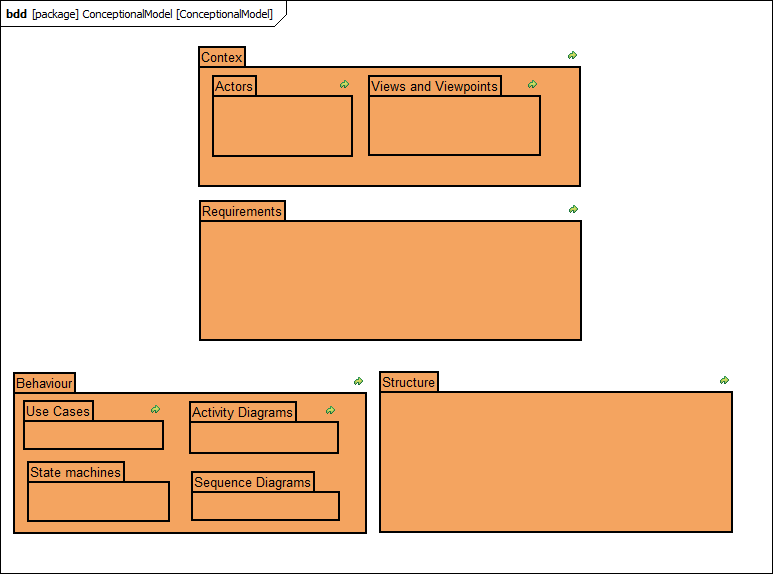
\includegraphics[scale=0.45]{ConceptionalModel_ConceptionalModel.png}
					\caption{Η δομή του μοντέλου Σύλληψης}
					\label{φωτ:Η δομή του μοντέλου Σύλληψης}
				\end{figure}
				
				\begin{figure}[hp]
					\centering
					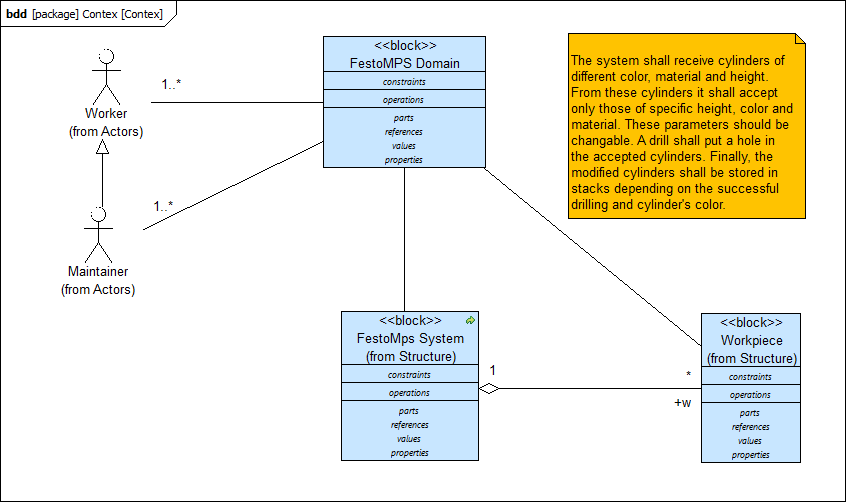
\includegraphics[scale=0.45]{ConceptionalModel_Contex.png}
					\caption{Ο χώρος υλοποίησης του μοντέλου Σύλληψης}
					\label{φωτ:Ο χώρος υλοποίησης του μοντέλου Σύλληψης}
				\end{figure}
				
				\begin{figure}[hp]
					\centering
					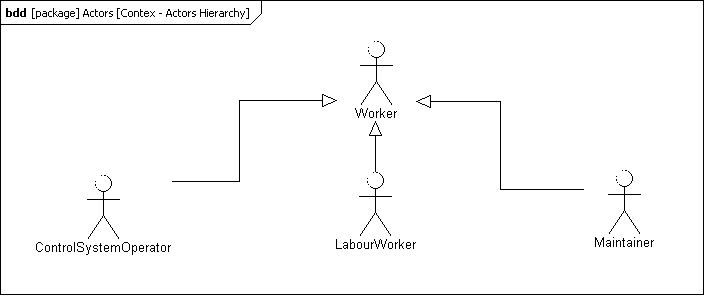
\includegraphics[scale=0.30]{ConceptionalModel_Contex-ActorsHierarchy.png}
					\caption{Οι ρόλοι του μοντέλου Σύλληψης}
					\label{φωτ:Οι ρόλοι του μοντέλου Σύλληψης}
				\end{figure}

%%%%%%%%%%%%%%%%%%%%%%%%%%%%%%%%%%%%%%%%%%%%%%%%%%%%%%%%%%%%%
%%%%%%%%%%%%%%		   							Υποενότητα		   					   %%%%%%%%%%%%%%%%%%%%
			\FloatBarrier
			\subsection{Πακέτο απαιτήσεων\index{πακέτο!απαιτήσεις}\index{απαιτήσεις!πακέτο} - Requirements package\index{requirements!package}\index{package!requirements}}
			\clearpage
				\begin{figure}[hp]
					\centering
					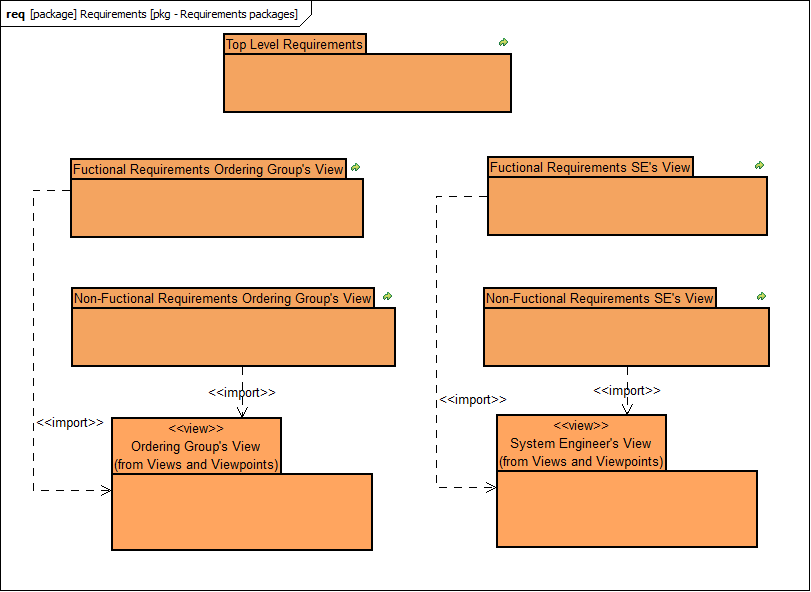
\includegraphics[scale=0.45]{ConceptionalModel_pkg-Requirementspackages.png}
					\caption{Η οργάνωση των απαιτήσεων στο μοντέλο Σύλληψης}
					\label{φωτ:Η οργάνωση των απαιτήσεων στο μοντέλο Σύλληψης}
				\end{figure}
				
				\begin{figure}[hp]
					\centering
					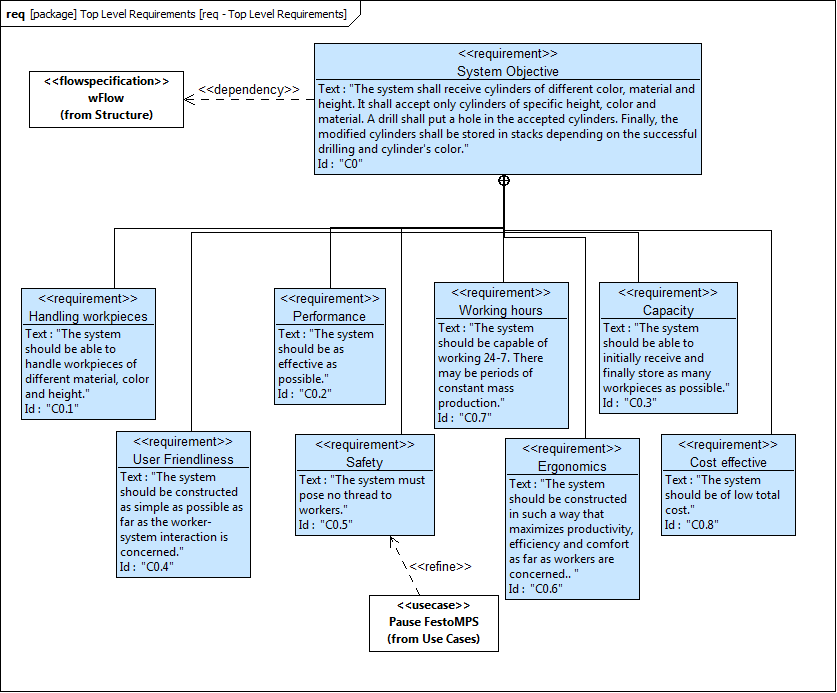
\includegraphics[scale=0.45]{ConceptionalModel_req-TopLevelRequirements.png}
					\caption{Οι γενικές απαιτήσεις του μοντέλου Σύλληψης}
					\label{φωτ:Οι γενικές απαιτήσεις του μοντέλου Σύλληψης}
				\end{figure}
				
				\begin{figure}[hp]
					\centering
					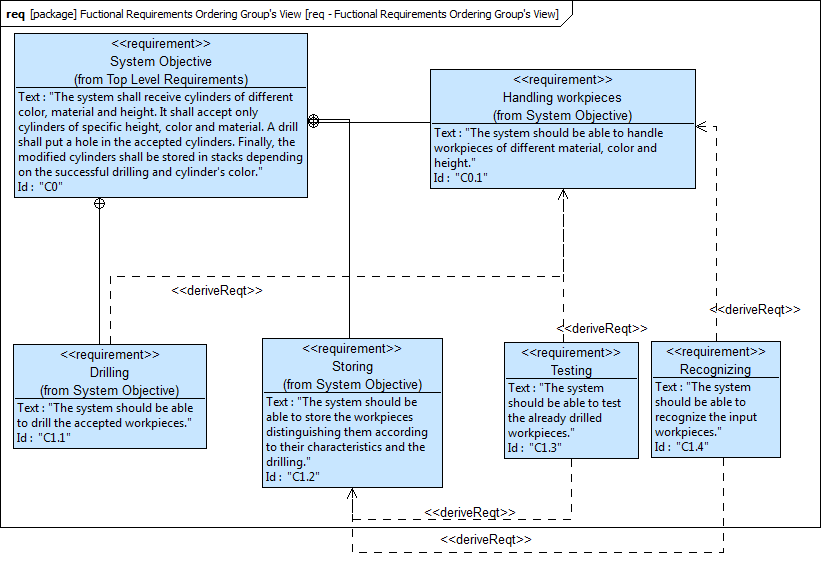
\includegraphics[scale=0.45]{ConceptionalModel_req-FuctionalRequirementsOrderingGroupsView.png}
					\caption{Οι λειτουργικές απαιτήσεις της ομάδας παραγγελίας στο μοντέλο Σύλληψης}
					\label{φωτ:Οι λειτουργικές απαιτήσεις της ομάδας παραγγελίας στο μοντέλο Σύλληψης}
				\end{figure}
				
				\begin{figure}[hp]
					\centering
					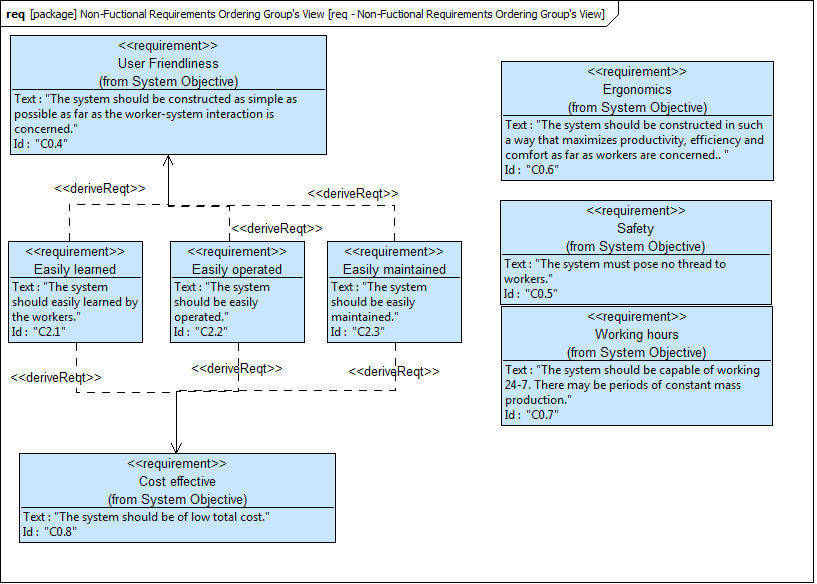
\includegraphics[scale=0.45]{ConceptionalModel_req-Non-FuctionalRequirementsOrderingGroupsView.png}
					\caption{Οι λοιπές απαιτήσεις της ομάδας παραγγελίας στο μοντέλο Σύλληψης}
					\label{φωτ:Οι λοιπές απαιτήσεις της ομάδας παραγγελίας στο μοντέλο Σύλληψης}
				\end{figure}
				
				\begin{figure}[hp]
					\centering
					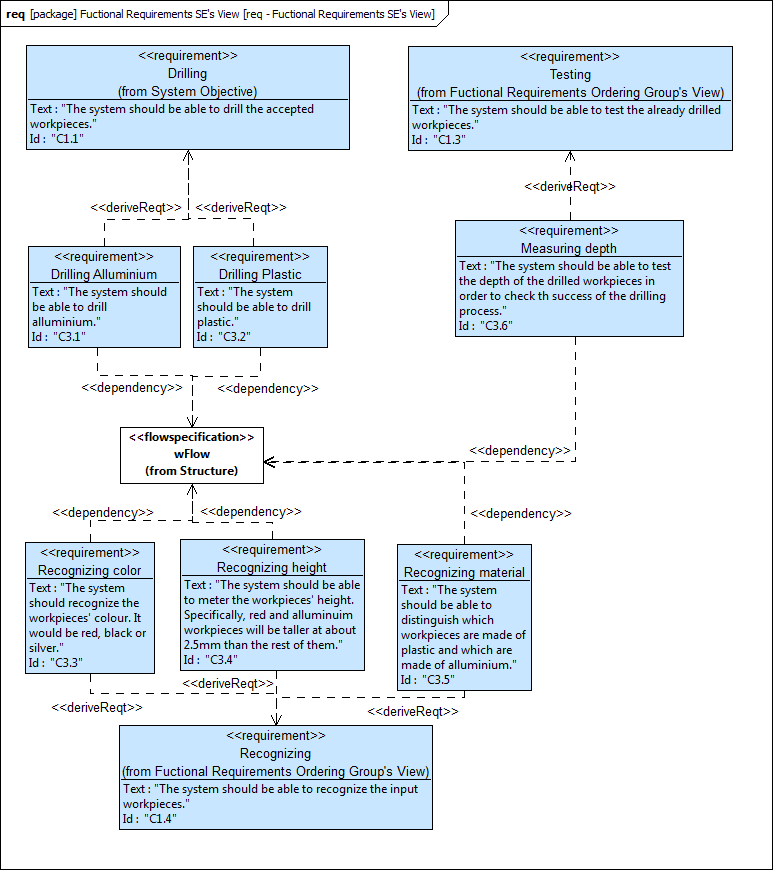
\includegraphics[scale=0.45]{ConceptionalModel_req-FuctionalRequirementsSEsView.png}
					\caption{Οι λειτουργικές απαιτήσεις του μηχανικού συστημάτων στο μοντέλο Σύλληψης}
					\label{φωτ:Οι λειτουργικές απαιτήσεις του μηχανικού συστημάτων στο μοντέλο Σύλληψης}
				\end{figure}
				
				\begin{figure}[hp]
					\centering
					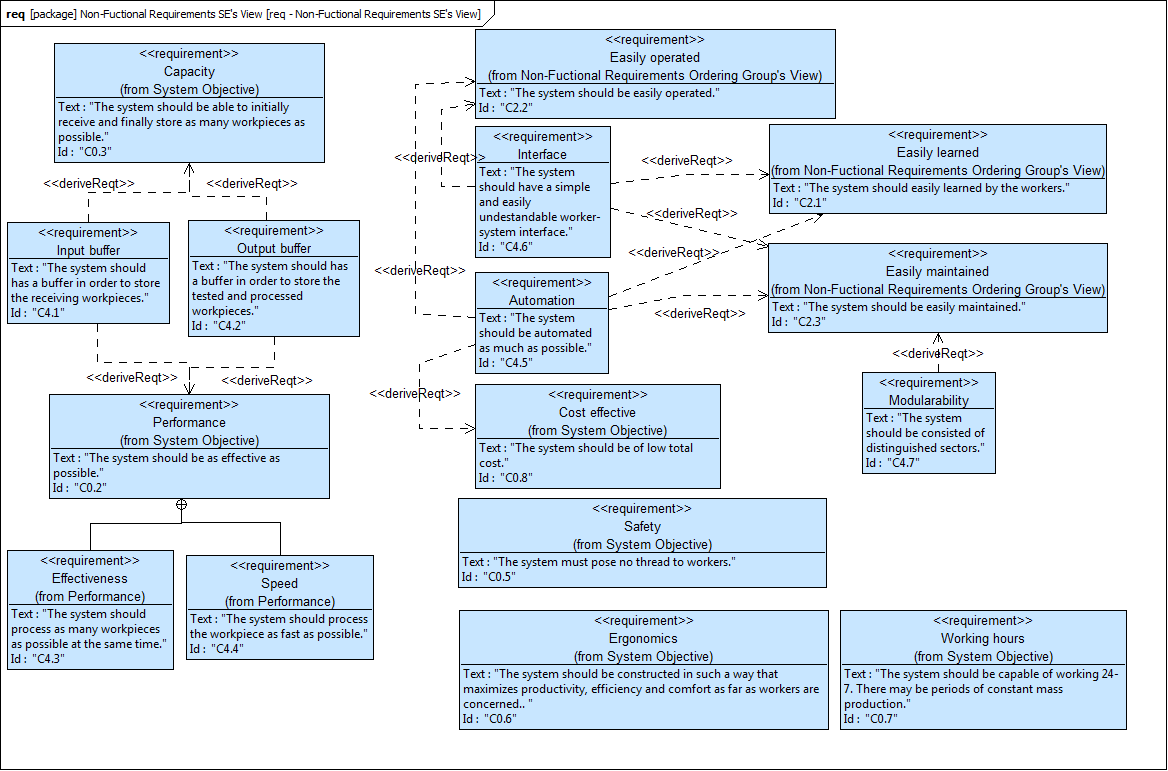
\includegraphics[scale=0.30]{ConceptionalModel_req-Non-FuctionalRequirementsSEsView.png}
					\caption{Οι λοιπές απαιτήσεις του μηχανικού συστημάτων στο μοντέλο Σύλληψης}
					\label{φωτ:Οι λοιπές απαιτήσεις του μηχανικού συστημάτων στο μοντέλο Σύλληψης}
				\end{figure}
			
%%%%%%%%%%%%%%%%%%%%%%%%%%%%%%%%%%%%%%%%%%%%%%%%%%%%%%%%%%%%%
%%%%%%%%%%%%%%		   							Υποενότητα		   					   %%%%%%%%%%%%%%%%%%%%		
			\FloatBarrier			
			\subsection{Πακέτο δομής\index{πακέτο!δομής}\index{δομή!πακέτο} - Structure package\index{structure!package}\index{package!structure}}

			\clearpage
				\begin{figure}[hp]
					\centering
					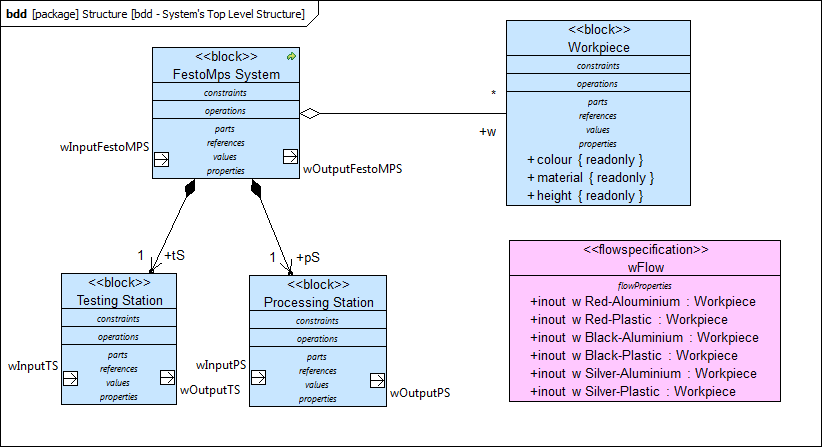
\includegraphics[scale=0.45]{ConceptionalModel_bdd-SystemsTopLevelStructure.png}
					\caption{Το bdd του συστήματος Festo MPS στο μοντέλο Σύλληψης}
					\label{φωτ:Το bdd του συστήματος Festo MPS στο μοντέλο Σύλληψης}
				\end{figure}
				\begin{figure}[hp]
					\centering
					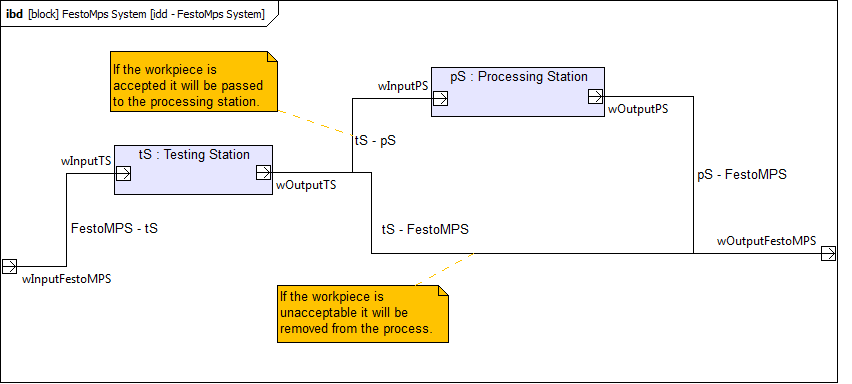
\includegraphics[scale=0.45]{ConceptionalModel_idd-FestoMpsSystem.png}
					\caption{To ibd του συστήματος Festo MPS στο μοντέλο Σύλληψης}
					\label{φωτ:To ibd του συστήματος Festo MPS στο μοντέλο Σύλληψης}
				\end{figure}
			
%%%%%%%%%%%%%%%%%%%%%%%%%%%%%%%%%%%%%%%%%%%%%%%%%%%%%%%%%%%%%
%%%%%%%%%%%%%%		   							Υποενότητα		   					   %%%%%%%%%%%%%%%%%%%%		
			\FloatBarrier
			\subsection{Πακέτο λειτουργίας\index{πακέτο!λειτουργίας}\index{λειτουργία!πακέτο} - Behaviour package\index{behavioul!package}\index{package!behaviour}}

			\clearpage
				\begin{figure}[hp]
					\centering
					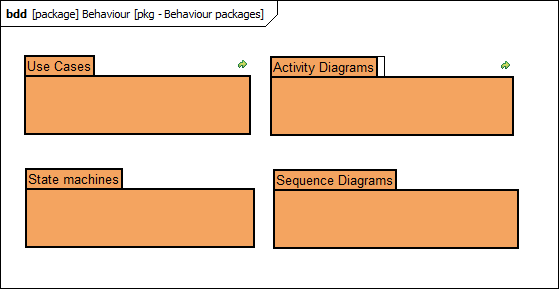
\includegraphics[scale=0.60]{ConceptionalModel_pkg-Behaviourpackages.png}
					\caption{Η οργάνωση του πακέτου λειτουργίας του συστήματος Festo MPS στο μοντέλο Σύλληψης}
					\label{φωτ: οργάνωση του πακέτου λειτουργίας του συστήματος Festo MPS στο μοντέλο Σύλληψης}
				\end{figure}
				\begin{figure}[hp]
					\centering
					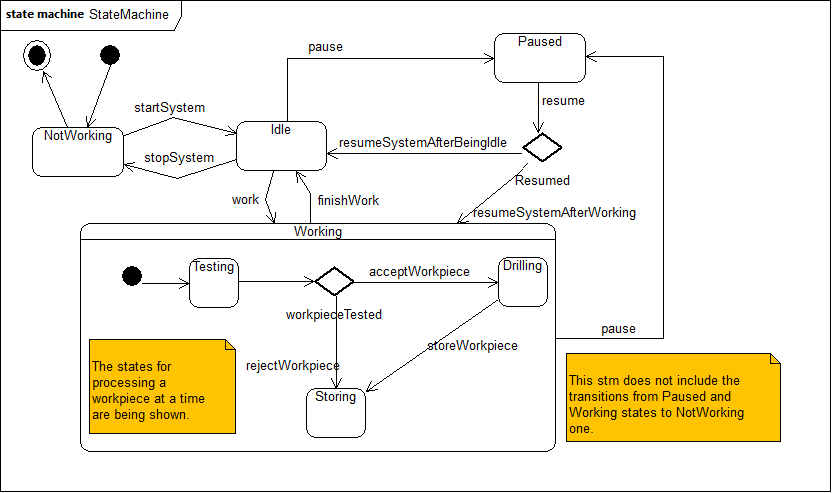
\includegraphics[scale=0.45]{ConceptionalModel_stm-SystemsTopLevelStateMachines.png}
					\caption{Οι καταστάσεις λειτουργίας του Festo MPS στο μοντέλο Σύλληψης}
					\label{φωτ:Οι καταστάσεις λειτουργίας του Festo MPS στο μοντέλο Σύλληψης}
				\end{figure}
				\begin{figure}[hp]
					\centering
					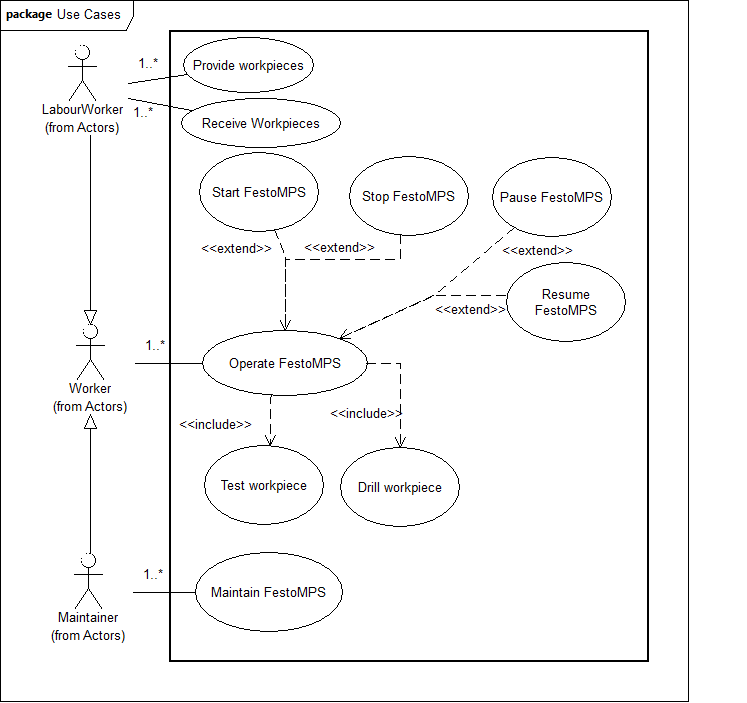
\includegraphics[scale=0.60]{ConceptionalModel_uc-SystemsTopLevelUseCases.png}
					\caption{Οι περιπτώσεις χρήσεις του Festo MPS στο μοντέλο Σύλληψης}
					\label{φωτ:Οι περιπτώσεις χρήσεις του Festo MPS στο μοντέλο Σύλληψης}
				\end{figure}
				\begin{figure}[hp]
					\centering
					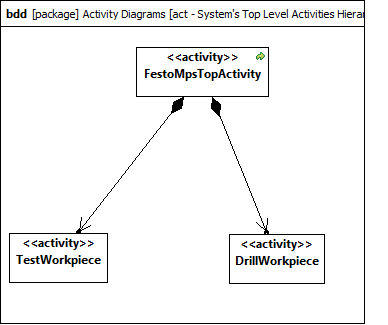
\includegraphics[scale=0.45]{ConceptionalModel_act-SystemsTopLevelActivitiesHierarchy.png}
					\caption{Η οργάνωση των Ενεργειών του Festo MPS στο μοντέλο Σύλληψης}
					\label{φωτ:Η οργάνωση των Ενεργειών του Festo MPS στο μοντέλο Σύλληψης}
				\end{figure}
				\begin{figure}[hp]
					\centering
					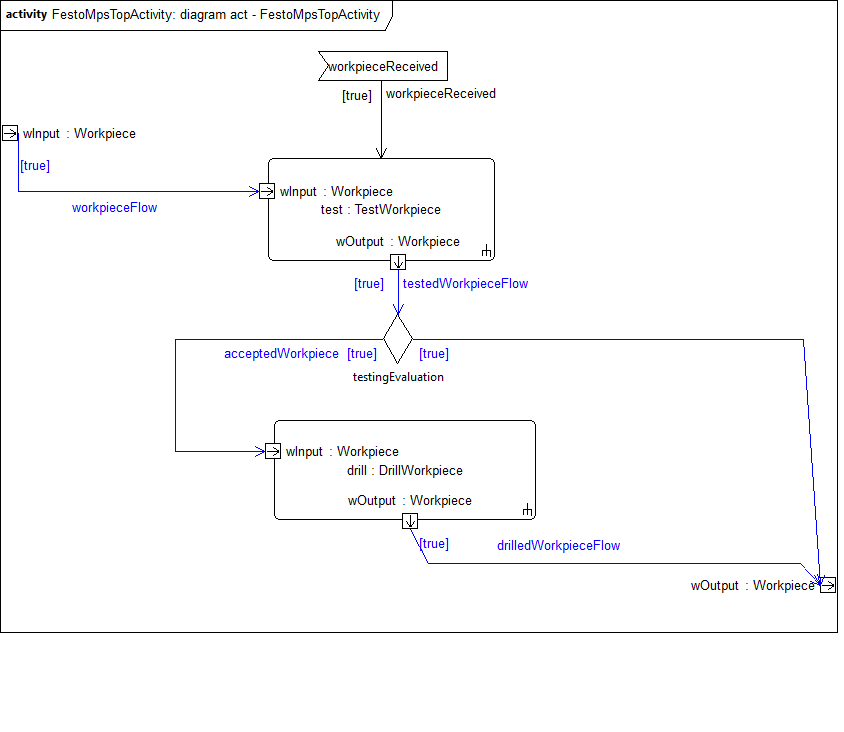
\includegraphics[scale=0.45]{ConceptionalModel_act-SystemsTopLevelActivity.png}
					\caption{Οι ενέργειες του Festo MPS στο μοντέλο Σύλληψης}
					\label{φωτ:Οι ενέργειες του Festo MPS στο μοντέλο Σύλληψης}
				\end{figure}
				\begin{figure}[hp]
					\centering
					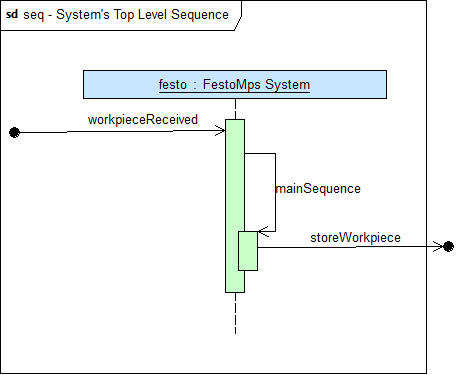
\includegraphics[scale=0.45]{ConceptionalModel_seq-SystemsTopLevelSequence.png}
					\caption{Το αφαιρετικό διάγραμμα ακολουθίας του μοντέλου Σύλληψης}
					\label{φωτ:Το αφαιρετικό διάγραμμα ακολουθίας του μοντέλου Σύλληψης}
				\end{figure}
				\begin{figure}[hp]
					\centering
					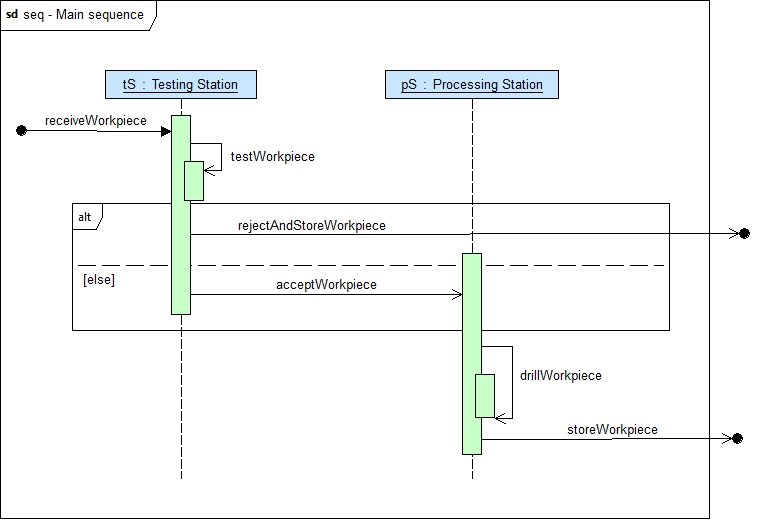
\includegraphics[scale=0.45]{ConceptionalModel_seq-MainSequence.png}
					\caption{Το διάγραμμα της κύριας ακολουθίας του Festo MPS στο μοντέλο Σύλληψης}
					\label{φωτ:Το διάγραμμα της κύριας ακολουθίας του Festo MPS στο μοντέλο Σύλληψης}
				\end{figure}

%%%%%%%%%%%%%%%%%%%%%%%%%%%%%%%%%%%%%%%%%%%%%%%%%%%%%%%%%%%%%
%%%%%%%%%%%%%%		   								 Ενότητα		   					   %%%%%%%%%%%%%%%%%%%%
%%%%%%%%%%%%%%%%%%%%%%%%%%%%%%%%%%%%%%%%%%%%%%%%%%%%%%%%%%%%%	
		\FloatBarrier		
		\section{Μοντέλο Ανάλυσης\index{μοντέλο!ανάλυσης} - Analysis Model\index{model!analysis}}
		
%%%%%%%%%%%%%%%%%%%%%%%%%%%%%%%%%%%%%%%%%%%%%%%%%%%%%%%%%%%%%
%%%%%%%%%%%%%%		   							Υποενότητα		   					   %%%%%%%%%%%%%%%%%%%%		
			\FloatBarrier
			\subsection{Χώρος υλοποίησης συστήματος\index{χώρος υλοποίησης} - Contex\index{contex}}

			\clearpage
				\begin{figure}[hp]
					\centering
					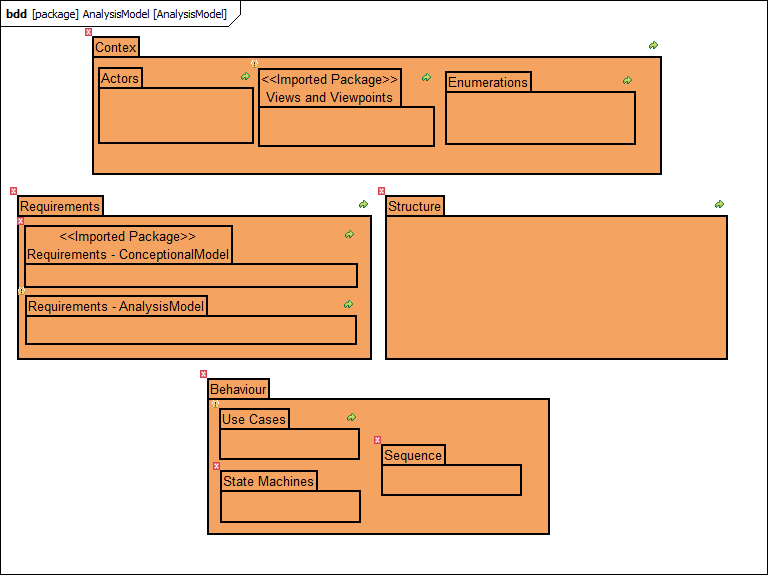
\includegraphics[scale=0.45]{AnalysisModel_AnalysisModel.png}
					\caption{Η δομή του μοντέλου Ανάλυσης}
					\label{φωτ:Η δομή του μοντέλου Ανάλυσης}
				\end{figure}
				
				\begin{figure}[hp]
					\centering
					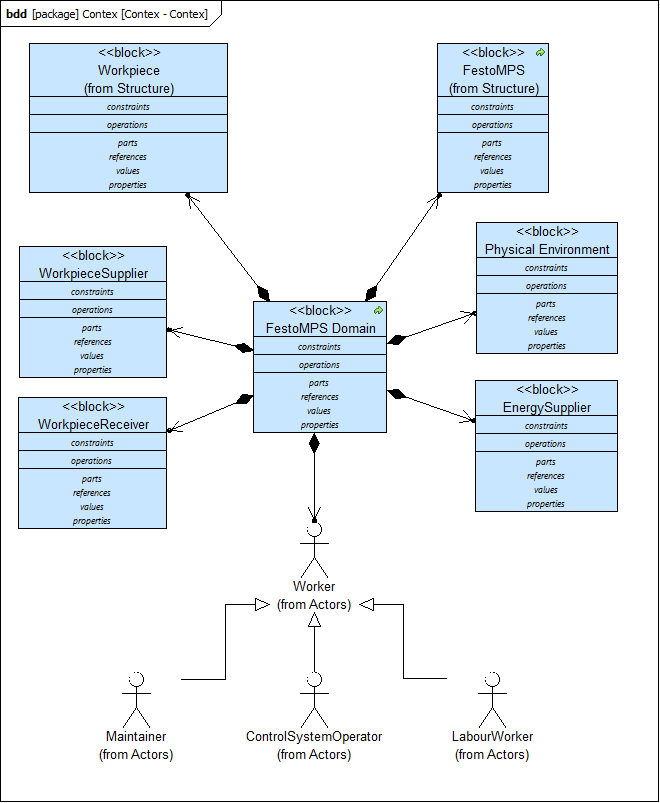
\includegraphics[scale=0.45]{AnalysisModel_Contex-Contex.png}
					\caption{Ο χώρος υλοποίησης του μοντέλου Ανάλυσης}
					\label{φωτ:Ο χώρος υλοποίησης του μοντέλου Ανάλυσης}
				\end{figure}
				
				\begin{figure}[hp]
					\centering
					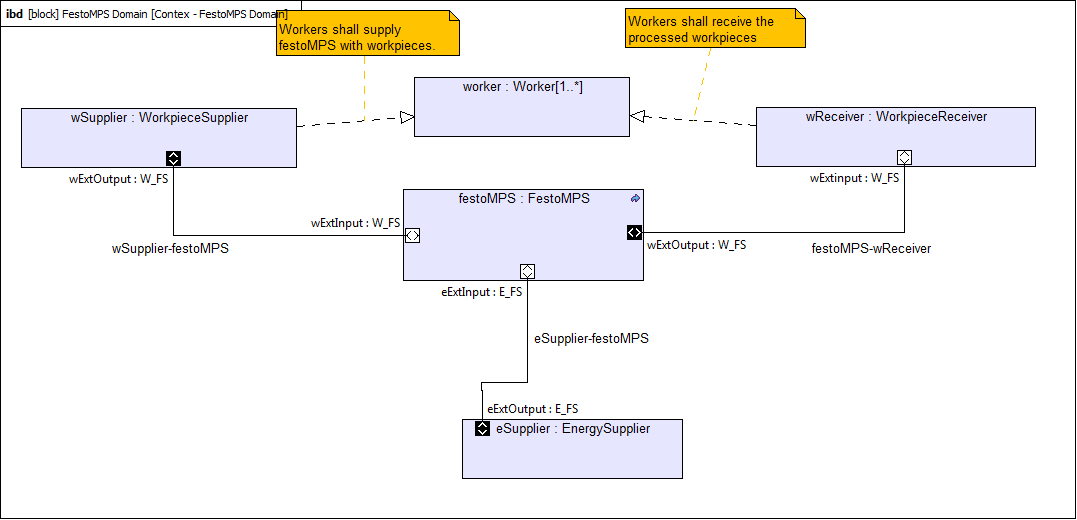
\includegraphics[scale=0.30]{AnalysisModel_Contex-FestoMPSDomain.png}
					\caption{Η σχέση του συστήματος με τον χώρο υλοποίησης του στο μοντέλο Ανάλυσης}
					\label{φωτ:Η σχέση του συστήματος με τον χώρο υλοποίησης του στο μοντέλο Ανάλυσης}
				\end{figure}
				
				\begin{figure}[hp]
					\centering
					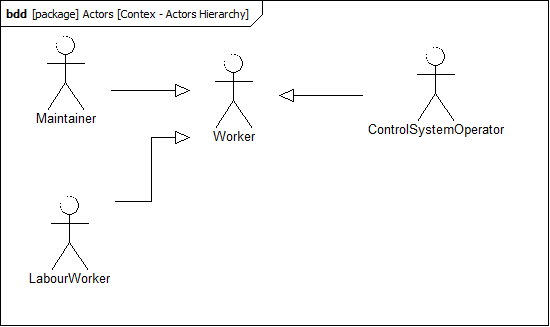
\includegraphics[scale=0.50]{AnalysisModel_Contex-ActorsHierarchy.png}
					\caption{Οι ρόλοι του μοντέλου Ανάλυσης}
					\label{φωτ:Οι ρόλοι του μοντέλου Ανάλυσης}
				\end{figure}
				
				\begin{figure}[hp]
					\centering
					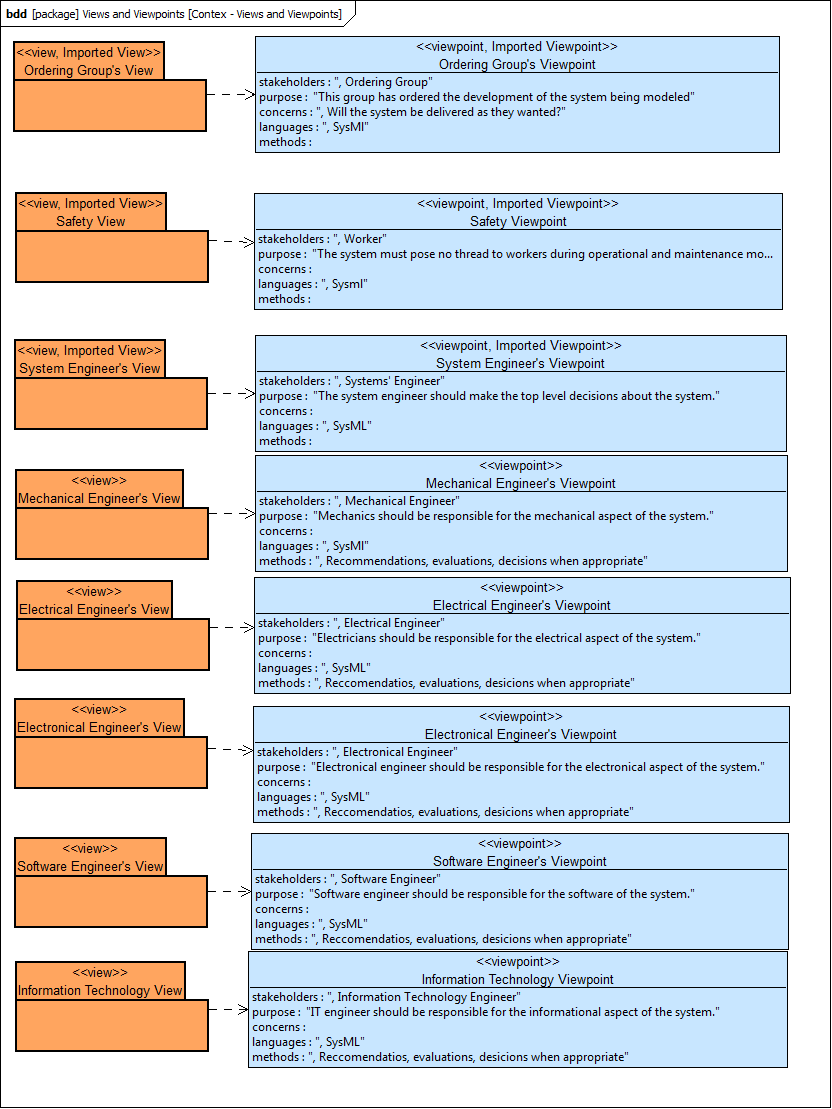
\includegraphics[scale=0.30]{AnalysisModel_Contex-ViewsandViewpoints.png}
					\caption{Οι όψεις του μοντέλου Ανάλυσης}
					\label{φωτ:Οι όψεις του μοντέλου Ανάλυσης}
				\end{figure}
				
				\begin{figure}[hp]
					\centering
					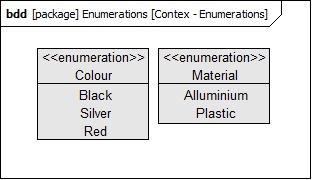
\includegraphics[scale=0.50]{AnalysisModel_Contex-Enumerations.png}
					\caption{Οι "απαριθμήσεις" του μοντέλου Ανάλυσης}
					\label{φωτ:Οι "απαριθμήσεις" του μοντέλου Ανάλυσης}
				\end{figure}		

%%%%%%%%%%%%%%%%%%%%%%%%%%%%%%%%%%%%%%%%%%%%%%%%%%%%%%%%%%%%%
%%%%%%%%%%%%%%		   							Υποενότητα		   					   %%%%%%%%%%%%%%%%%%%%			
			\FloatBarrier
			\subsection{Πακέτο απαιτήσεων\index{πακέτο!απαιτήσεις}\index{απαιτήσεις!πακέτο} - Requirements package\index{requirements!package}\index{package!requirements}}

			\clearpage
			\begin{figure}[hp]
					\centering
					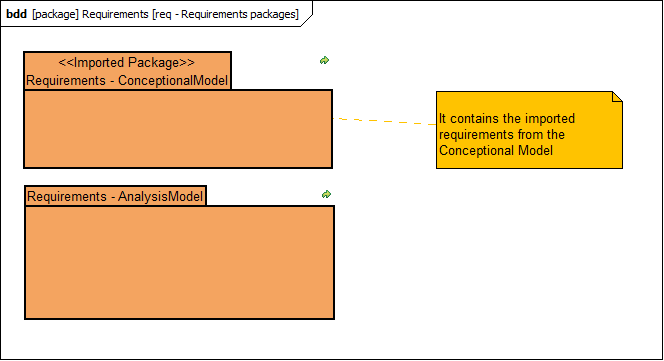
\includegraphics[scale=0.30]{AnalysisModel_req-Requirementspackages.png}
					\caption{Η δομή των απαιτήσεων του μοντέλου Ανάλυσης}
					\label{φωτ:Η δομή των απαιτήσεων του μοντέλου Ανάλυσης}
			\end{figure}
			
			\begin{figure}[hp]
					\centering
					\includegraphics[scale=0.30]{AnalysisModel_pkg-ImportedRequirementspackages.png}
					\caption{Η δομή των απαιτήσεων του μοντέλου Ανάλυσης που έχουν εισαχθεί από το μοντέλο Σύλληψης}
					\label{φωτ:Η δομή των απαιτήσεων του μοντέλου Ανάλυσης που έχουν εισαχθεί από το μοντέλο Σύλληψης}
			\end{figure}
			
			\begin{figure}[hp]
					\centering
					\includegraphics[scale=0.45]{AnalysisModel_req-TopLevelRequirements.png}
					\caption{Οι γενικές απαιτήσεις του μοντέλου Ανάλυσης που έχουν εισαχθεί από το μοντέλο σύλληψης}
					\label{φωτ:Οι γενικές απαιτήσεις του μοντέλου Ανάλυσης που έχουν εισαχθεί από το μοντέλο σύλληψης}
			\end{figure}
				
			\begin{figure}[hp]
					\centering
					\includegraphics[scale=0.45]{AnalysisModel_req-FuctionalRequirementsOrderingGroupsView.png}
					\caption{Οι λειτουργικές απαιτήσεις της ομάδας παραγγελίας στο μοντέλο Ανάλυσης που έχουν εισαχθεί από το μοντέλο Σύλληψης}
					\label{φωτ:Οι λειτουργικές απαιτήσεις της ομάδας παραγγελίας στο μοντέλο Ανάλυσης που έχουν εισαχθεί από το μοντέλο Σύλληψης}
			\end{figure}
				
			\begin{figure}[hp]
					\centering
					\includegraphics[scale=0.45]{AnalysisModel_req-Non-FuctionalRequirementsOrderingGroupsView.png}
					\caption{Οι λοιπές απαιτήσεις της ομάδας παραγγελίας στο μοντέλο Ανάλυσης που έχουν εισαχθεί από το μοντέλο Σύλληψης}
				\label{φωτ:Οι λοιπές απαιτήσεις της ομάδας παραγγελίας στο μοντέλο Ανάλυσης που έχουν εισαχθεί από το μοντέλο Σύλληψης}
			\end{figure}
				
			\begin{figure}[hp]
					\centering
					\includegraphics[scale=0.45]{AnalysisModel_req-FuctionalRequirementsSEsView.png}
					\caption{Οι λειτουργικές απαιτήσεις του μηχανικού συστημάτων στο μοντέλο Ανάλυσης που έχουν εισαχθεί από το μοντέλο Σύλληψης}
					\label{φωτ:Οι λειτουργικές απαιτήσεις του μηχανικού συστημάτων στο μοντέλο Ανάλυσης που έχουν εισαχθεί από το μοντέλο Σύλληψης}
			\end{figure}
				
			\begin{figure}[hp]
					\centering
					\includegraphics[scale=0.30]{AnalysisModel_req-Non-FuctionalRequirementsSEsView.png}
					\caption{Οι λοιπές απαιτήσεις του μηχανικού συστημάτων στο μοντέλο Ανάλυσης που έχουν εισαχθεί από το μοντέλο Σύλληψης}
					\label{φωτ:Οι λοιπές απαιτήσεις του μηχανικού συστημάτων στο μοντέλο Ανάλυσης που έχουν εισαχθεί από το μοντέλο Σύλληψης}
			\end{figure}
			
			\begin{figure}[hp]
					\centering
					\includegraphics[scale=0.30]{AnalysisModel_req-StationRequirements(DistributionStation).png}
					\caption{Οι απαιτήσεις του σταθμού διανομής στο μοντέλο Ανάλυσης}
					\label{φωτ:Οι απαιτήσεις του σταθμού διανομής στο μοντέλο Ανάλυσης}
			\end{figure}
			
			\begin{figure}[hp]
					\centering
					\includegraphics[scale=0.30]{AnalysisModel_req-StationRequirements(TestingStation).png}
					\caption{Οι απαιτήσεις του σταθμού ελέγχου στο μοντέλο Ανάλυσης}
					\label{φωτ:Οι απαιτήσεις του σταθμού ελέγχου στο μοντέλο Ανάλυσης}
			\end{figure}
			
			\begin{figure}[hp]
					\centering
					\includegraphics[scale=0.30]{AnalysisModel_req-StationRequirements(ProcessingStation).png}
					\caption{Οι απαιτήσεις του σταθμού επεξεργασίας στο μοντέλο Ανάλυσης}
					\label{φωτ:Οι απαιτήσεις του σταθμού επεξεργασίας στο μοντέλο Ανάλυσης}
			\end{figure}
			
			\begin{figure}[hp]
					\centering
					\includegraphics[scale=0.30]{AnalysisModel_req-StationRequirements(WarehousingStation).png}
					\caption{Οι απαιτήσεις του σταθμού αποθήκευσης στο μοντέλο Ανάλυσης}
					\label{φωτ:Οι απαιτήσεις του σταθμού αποθήκευσης στο μοντέλο Ανάλυσης}
			\end{figure}
			
			\begin{figure}[hp]
					\centering
					\includegraphics[scale=0.20]{AnalysisModel_req-Satisfaction(ConceptionalModelsRequirements).png}
					\caption{Η πλήρωση των απαιτήσεων του μοντέλου Σύλληψης}
					\label{φωτ:Η πλήρωση των απαιτήσεων του μοντέλου Σύλληψης}
			\end{figure}
			
			\begin{figure}[hp]
					\centering
					\includegraphics[scale=0.30]{AnalysisModel_req-Satisfaction(DistributionStationsRequirements).png}
					\caption{Η πλήρωση των απαιτήσεων του σταθμού διανομής στο μοντέλο Ανάλυσης}
					\label{φωτ:Η πλήρωση των απαιτήσεων του σταθμού διανομής στο μοντέλο Ανάλυσης}
			\end{figure}
			
			\begin{figure}[hp]
					\centering
					\includegraphics[scale=0.30]{AnalysisModel_req-Satisfaction(TestingStationsRequirements).png}
					\caption{Η πλήρωση των απαιτήσεων του σταθμού ελέγχου στο μοντέλο Ανάλυσης}
					\label{φωτ:Η πλήρωση των απαιτήσεων του σταθμού ελέγχου στο μοντέλο Ανάλυσης}
			\end{figure}
			
			\begin{figure}[hp]
					\centering
					\includegraphics[scale=0.30]{AnalysisModel_req-Satisfaction(ProcessingStationsRequirements).png}
					\caption{Η πλήρωση των απαιτήσεων του σταθμού επεξεργασίας στο μοντέλο Ανάλυσης}
					\label{φωτ:Η πλήρωση των απαιτήσεων του σταθμού επεξεργασίας στο μοντέλο Ανάλυσης}
			\end{figure}
			
			\begin{figure}[hp]
					\centering
					\includegraphics[scale=0.30]{AnalysisModel_req-Satisfaction(WarehousingStationsRequirements).png}
					\caption{Η πλήρωση των απαιτήσεων του σταθμού αποθήκευσης στο μοντέλο Ανάλυσης}
					\label{φωτ:Η πλήρωση των απαιτήσεων του σταθμού αποθήκευσης στο μοντέλο Ανάλυσης}
			\end{figure}
			
			\begin{figure}[hp]
					\centering
					\includegraphics[scale=0.30]{AnalysisModel_req-StationRequirements(CentralControlStation).png}
					\caption{Η πλήρωση των απαιτήσεων του σταθμού κεντρικού ελέγχου στο μοντέλο Ανάλυσης}
					\label{φωτ:Η πλήρωση των απαιτήσεων του σταθμού κεντρικού ελέγχου στο μοντέλο Ανάλυσης}
			\end{figure}

%%%%%%%%%%%%%%%%%%%%%%%%%%%%%%%%%%%%%%%%%%%%%%%%%%%%%%%%%%%%%
%%%%%%%%%%%%%%		   							Υποενότητα		   					   %%%%%%%%%%%%%%%%%%%%			
			\FloatBarrier
			\subsection{Πακέτο δομής\index{πακέτο!δομής}\index{δομή!πακέτο} - Structure package\index{structure!package}\index{package!structure}}

			\clearpage
			\begin{figure}[hp]
					\centering
					\includegraphics[scale=0.30]{AnalysisModel_bdd-HierarchyofTopLevelBlocks.png}
					\caption{Η ιεραρχική διάρθρωση των βασικών δομικών στοιχείων στο μοντέλο Ανάλυσης}
					\label{φωτ:Η ιεραρχική διάρθρωση των βασικών δομικών στοιχείων στο μοντέλο Ανάλυσης}
			\end{figure}
			
			\begin{figure}[hp]
					\centering
					\includegraphics[scale=0.30]{AnalysisModel_bdd-Hierarchyof2ndLevelBlocks.png}
					\caption{Η ιεραρχική διάρθρωση των δευτερευόντων δομικών στοιχείων στο μοντέλο Ανάλυσης}
					\label{φωτ:Η ιεραρχική διάρθρωση των δευτερευόντων δομικών στοιχείων στο μοντέλο Ανάλυσης}
			\end{figure}
			
			\begin{figure}[hp]
					\centering
					\includegraphics[scale=0.30]{AnalysisModel_bdd-FlowSpesifications.png}
					\caption{Οι τεκμηριώσεις των ροών στο μοντέλο Ανάλυσης}
					\label{φωτ:Οι τεκμηριώσεις των ροών στο μοντέλο Ανάλυσης}
			\end{figure}
			
			\begin{figure}[hp]
					\centering
					\includegraphics[scale=0.30]{AnalysisModel_bdd-Interfaces.png}
					\caption{Οι τεκμηριώσεις των διεπαφών στο μοντέλο Ανάλυσης}
					\label{φωτ:Οι τεκμηριώσεις των διεπαφών στο μοντέλο Ανάλυσης}
			\end{figure}
			
			\begin{figure}[hp]
					\centering
					\includegraphics[scale=0.30]{AnalysisModel_bdd-TopLevelStructureofFestoMPS.png}
					\caption{To bdd του Festo Mps στο μοντέλο Ανάλυσης}
					\label{φωτ:To bdd του Festo Mps στο μοντέλο Ανάλυσης}
			\end{figure}
			
			\begin{figure}[hp]
					\centering
					\includegraphics[scale=0.30]{AnalysisModel_ibd-FestoMPSconnectionsinvolvingworkpieces.png}
					\caption{To ibd του Festo MPS αναφερόμενο στις πρώτες ύλες στο μοντέλο Ανάλυσης}
					\label{φωτ:To ibd του Festo MPS αναφερόμενο στις πρώτες ύλες στο μοντέλο Ανάλυσης}
			\end{figure}
			
			\begin{figure}[hp]
					\centering
					\includegraphics[scale=0.30]{AnalysisModel_ibd-FestoMPSconnectionsinvolvingcentralcontrolstructuralconnections.png}
					\caption{To ibd του Festo MPS αναφερόμενο στις γραμμές ελέγχου στο μοντέλο Ανάλυσης}
					\label{φωτ:To ibd του Festo MPS αναφερόμενο στις γραμμές ελέγχου στο μοντέλο Ανάλυσης}
			\end{figure}
			
			\begin{figure}[hp]
					\centering
					\includegraphics[scale=0.30]{AnalysisModel_ibd-FestoMPSconnectionsinvolvingcentralcontrolinterfaces.png}
					\caption{To ibd του Festo MPS αναφερόμενο στις διεπαφές στο μοντέλο Ανάλυσης}
					\label{φωτ:To ibd του Festo MPS αναφερόμενο στις διεπαφές στο μοντέλο Ανάλυσης}
			\end{figure}
			
			\begin{figure}[hp]
					\centering
					\includegraphics[scale=0.30]{AnalysisModel_ibd-FestoMPSconnectionsinvolvingenergy.png}
					\caption{To ibd του Festo MPS αναφερόμενο στην ενέργεια στο μοντέλο Ανάλυσης}
					\label{φωτ:To ibd του Festo MPS αναφερόμενο στην ενέργεια στο μοντέλο Ανάλυσης}
			\end{figure}
			
			\begin{figure}[hp]
					\centering
					\includegraphics[scale=0.30]{AnalysisModel_bdd-DistributionStationsStructure.png}
					\caption{To bdd του σταθμού διανομής στο μοντέλο Ανάλυσης}
					\label{φωτ:To bdd του σταθμού διανομής στο μοντέλο Ανάλυσης}
			\end{figure}
			
			\begin{figure}[hp]
					\centering
					\includegraphics[scale=0.30]{AnalysisModel_ibd-DistributionStation.png}
					\caption{To ibd του σταθμού διανομής στο μοντέλο Ανάλυσης}
					\label{φωτ:To ibd του σταθμού διανομής στο μοντέλο Ανάλυσης}
			\end{figure}
			
			\begin{figure}[hp]
					\centering
					\includegraphics[scale=0.30]{AnalysisModel_bdd-TestingStationsStructure.png}
					\caption{To bdd του σταθμού ελέγχου στο μοντέλο Ανάλυσης}
					\label{φωτ:To bdd του σταθμού ελέγχου Festo Mps στο μοντέλο Ανάλυσης}
			\end{figure}
			
			\begin{figure}[hp]
					\centering
					\includegraphics[scale=0.30]{AnalysisModel_ibd-TestingStationconnectionsinvolvingworkpieces.png}
					\caption{To ibd του σταθμού ελέγχου αναφερόμενο στις πρώτες ύλες στο μοντέλο Ανάλυσης}
					\label{φωτ:To ibd του σταθμού ελέγχου αναφερόμενο στις πρώτες ύλες στο μοντέλο Ανάλυσης}
			\end{figure}
			
			\begin{figure}[hp]
					\centering
					\includegraphics[scale=0.30]{AnalysisModel_ibd-TestingStationconnectionsinvolvingcontrol.png}
					\caption{To ibd του σταθμού ελέγχου αναφερόμενο στον έλεγχο στο μοντέλο Ανάλυσης}
					\label{φωτ:To ibd του σταθμού ελέγχου αναφερόμενο στον έλεγχο στο μοντέλο Ανάλυσης}
			\end{figure}
			
			\begin{figure}[hp]
					\centering
					\includegraphics[scale=0.30]{AnalysisModel_ibd-RecognizingModule.png}
					\caption{To ibd της μονάδας αναγνώρισης στο μοντέλο Ανάλυσης}
					\label{φωτ:To ibd της μονάδας αναγνώρισης στο μοντέλο Ανάλυσης}
			\end{figure}
			
			\begin{figure}[hp]
					\centering
					\includegraphics[scale=0.30]{AnalysisModel_bdd-ProcessingStationsStructure.png}
					\caption{To bdd του σταθμού επεξεργασίας στο μοντέλο Ανάλυσης}
					\label{φωτ:To bdd του σταθμού επεξεργασίας στο μοντέλο Ανάλυσης}
			\end{figure}
			
			\begin{figure}[hp]
					\centering
					\includegraphics[scale=0.30]{AnalysisModel_ibd-ProcessingStation.png}
					\caption{To ibd του σταθμού επεξεργασίας στο μοντέλο Ανάλυσης}
					\label{φωτ:To ibd του σταθμού επεξεργασίας στο μοντέλο Ανάλυσης}
			\end{figure}
			
			\begin{figure}[hp]
					\centering
					\includegraphics[scale=0.50]{AnalysisModel_bdd-WarehouseStationsStructure.png}
					\caption{To bdd του σταθμού αποθήκευσης στο μοντέλο Ανάλυσης}
					\label{φωτ:To bdd του σταθμού αποθήκευσης στο μοντέλο Ανάλυσης}
			\end{figure}
			
			\clearpage
			\begin{figure}[hp]
					\centering
					\includegraphics[scale=0.50]{AnalysisModel_ibd-WarehouseStation.png}
					\caption{To ibd του σταθμού αποθήκευσης στο μοντέλο Ανάλυσης}
					\label{φωτ:To ibd του σταθμού αποθήκευσης στο μοντέλο Ανάλυσης}
			\end{figure}
			
			\begin{figure}[hp]
					\centering
					\includegraphics[scale=0.50]{AnalysisModel_bdd-CentralControlStationsStructure.png}
					\caption{To bdd του σταθμού κεντρικού ελέχου στο μοντέλο Ανάλυσης}
					\label{φωτ:To bdd του σταθμού κεντρικού ελέγχου στο μοντέλο Ανάλυσης}
			\end{figure}
			
			\begin{figure}[hp]
					\centering
					\includegraphics[scale=0.50]{AnalysisModel_ibd-CentralControlStation.png}
					\caption{To ibd του σταθμού κεντρικού ελέγχου στο μοντέλο Ανάλυσης}
					\label{φωτ:To ibd του σταθμού κεντρικού ελέγχου στο μοντέλο Ανάλυσης}
			\end{figure}

%%%%%%%%%%%%%%%%%%%%%%%%%%%%%%%%%%%%%%%%%%%%%%%%%%%%%%%%%%%%%
%%%%%%%%%%%%%%		   							Υποενότητα		   					   %%%%%%%%%%%%%%%%%%%%			
			\FloatBarrier
			\subsection{Πακέτο λειτουργίας\index{πακέτο!λειτουργίας}\index{λειτουργία!πακέτο} - Behaviour package\index{behavioul!package}\index{package!behaviour}}

			\clearpage
			\begin{figure}[hp]
					\centering
					\includegraphics[scale=0.30]{AnalysisModel_uc-TopLevelUseCases.png}
					\caption{Οι περιπτώσεις χρήσεις του Festo MPS στο μοντέλο Ανάλυσης}
					\label{φωτ:Οι περιπτώσεις χρήσεις του Festo MPS στο μοντέλο Ανάλυσης}
			\end{figure}
			
			\begin{figure}[hp]
					\centering
					\includegraphics[scale=0.30]{AnalysisModel_stm-FestoMpsTopLevelStates.png}
					\caption{Το διάγραμμα καταστάσεων του Festo MPS στο μοντέλο Ανάλυσης}
					\label{φωτ:Το διάγραμμα καταστάσεων του Festo MPS στο μοντέλο Ανάλυσης}
			\end{figure}
			
			\begin{figure}[hp]
					\centering
					\includegraphics[scale=0.30]{AnalysisModel_seq-FestoMpsTopLevelSequence.png}
					\caption{Το διάγραμμα ακολουθίας του Festo MPS στο μοντέλο Ανάλυσης}
					\label{φωτ:Το διάγραμμα ακολουθίας του Festo MPS στο μοντέλο Ανάλυσης}
			\end{figure}
			
			\begin{figure}[hp]
					\centering
					\includegraphics[scale=0.30]{AnalysisModel_seq-PowerOn.png}
					\caption{Το διάγραμμα ακολουθίας για την ενεργοποίηση του Festo MPS στο μοντέλο Ανάλυσης}
					\label{φωτ:Το διάγραμμα ακολουθίας για την ενεργοποίηση του Festo MPS στο μοντέλο Ανάλυσης}
			\end{figure}
			
			\begin{figure}[hp]
					\centering
					\includegraphics[scale=0.30]{AnalysisModel_seq-InitializeSystem.png}
					\caption{Το διάγραμμα ακολουθίας για την αρχικοποίηση του Festo MPS στο μοντέλο Ανάλυσης}
					\label{φωτ:Το διάγραμμα ακολουθίας για την αρχικοποίηση του Festo MPS στο μοντέλο Ανάλυσης}
			\end{figure}
			
			\begin{figure}[hp]
					\centering
					\includegraphics[scale=0.30]{AnalysisModel_seq-TerminateSystem.png}
					\caption{Το διάγραμμα ακολουθίας για τον τερματισμό εκκίνηση του Festo MPS στο μοντέλο Ανάλυσης}
					\label{φωτ:Το διάγραμμα ακολουθίας για τον τερματισμό του Festo MPS στο μοντέλο Ανάλυσης}
			\end{figure}
			
			\begin{figure}[hp]
					\centering
					\includegraphics[scale=0.30]{AnalysisModel_seq-PowerOff.png}
					\caption{Το διάγραμμα ακολουθίας για την απενεργοποίηση του Festo MPS στο μοντέλο Ανάλυσης}
					\label{φωτ:Το διάγραμμα ακολουθίας για την απενεργοποίηση του Festo MPS στο μοντέλο Ανάλυσης}
			\end{figure}
			
			\begin{figure}[hp]
					\centering
					\includegraphics[scale=0.30]{AnalysisModel_uc-DistributionStationsUseCases.png}
					\caption{Οι περιπτώσεις χρήσεις του σταθμού διανομής στο μοντέλο Ανάλυσης}
					\label{φωτ:Οι περιπτώσεις χρήσεις του σταθμού διανομής στο μοντέλο Ανάλυσης}
			\end{figure}
			
			\begin{figure}[hp]
					\centering
					\includegraphics[scale=0.30]{AnalysisModel_seq-DistributionStation(normalprocess).png}
					\caption{Το διάγραμμα ακολουθίας του σταθμού διανομής στο μοντέλο Ανάλυσης}
					\label{φωτ:Το διάγραμμα ακολουθίας του σταθμού διανομής στο μοντέλο Ανάλυσης}
			\end{figure}

			\begin{figure}[hp]
					\centering
					\includegraphics[scale=0.30]{AnalysisModel_uc-TestingStationsUseCases.png}
					\caption{Οι περιπτώσεις χρήσεις του σταθμού ελέγχου στο μοντέλο Ανάλυσης}
					\label{φωτ:Οι περιπτώσεις χρήσεις του σταθμού ελέγχου στο μοντέλο Ανάλυσης}
			\end{figure}
			
			\begin{figure}[hp]
					\centering
					\includegraphics[scale=0.30]{AnalysisModel_stm-TestingStation(Testingstate).png}
					\caption{Το διάγραμμα καταστάσεων του σταθμού ελέγχου στο μοντέλο Ανάλυσης}
					\label{φωτ:Το διάγραμμα καταστάσεων του σταθμού ελέγχου στο μοντέλο Ανάλυσης}
			\end{figure}
			
			\begin{figure}[hp]
					\centering
					\includegraphics[scale=0.30]{AnalysisModel_seq-TestingStation(normalprocess).png}
					\caption{Το διάγραμμα ακολουθίας του σταθμού ελέγχου στο μοντέλο Ανάλυσης}
					\label{φωτ:Το διάγραμμα ακολουθίας του σταθμού ελέγχου στο μοντέλο Ανάλυσης}
			\end{figure}
			
			\begin{figure}[hp]
					\centering
					\includegraphics[scale=0.30]{AnalysisModel_uc-ProcessingStationsUseCases.png}
					\caption{Οι περιπτώσεις χρήσεις του σταθμού επεξεργασίας στο μοντέλο Ανάλυσης}
					\label{φωτ:Οι περιπτώσεις χρήσεις του σταθμού επεξεργασίας στο μοντέλο Ανάλυσης}
			\end{figure}
			
			\begin{figure}[hp]
					\centering
					\includegraphics[scale=0.30]{AnalysisModel_stm-ProcessingStation(Processingstate).png}
					\caption{Το διάγραμμα καταστάσεων του σταθμού επεξεργασίας στο μοντέλο Ανάλυσης}
					\label{φωτ:Το διάγραμμα καταστάσεων του σταθμού επεξεργασίας στο μοντέλο Ανάλυσης}
			\end{figure}
			
			\begin{figure}[hp]
					\centering
					\includegraphics[scale=0.30]{AnalysisModel_seq-ProcessingStation(normalprocess).png}
					\caption{Το διάγραμμα ακολουθίας του σταθμού επεξεργασίας στο μοντέλο Ανάλυσης}
					\label{φωτ:Το διάγραμμα ακολουθίας του σταθμού επεξεργασίας στο μοντέλο Ανάλυσης}
			\end{figure}
			
			\begin{figure}[hp]
					\centering
					\includegraphics[scale=0.30]{AnalysisModel_uc-WarehousingStationsUseCases.png}
					\caption{Οι περιπτώσεις χρήσεις του σταθμού αποθήκευσης στο μοντέλο Ανάλυσης}
					\label{φωτ:Οι περιπτώσεις χρήσεις του σταθμού αποθήκευσης στο μοντέλο Ανάλυσης}
			\end{figure}

			\begin{figure}[hp]
					\centering
					\includegraphics[scale=0.30]{AnalysisModel_seq-WarehousingStation(normalprocess).png}
					\caption{Το διάγραμμα ακολουθίας του σταθμού αποθήκευσης στο μοντέλο Ανάλυσης}
					\label{φωτ:Το διάγραμμα ακολουθίας του σταθμού αποθήκευσης στο μοντέλο Ανάλυσης}
			\end{figure}
			
			\begin{figure}[hp]
					\centering
					\includegraphics[scale=0.30]{AnalysisModel_uc-CentralEnergyStationsUseCases.png}
					\caption{Οι περιπτώσεις χρήσεις του σταθμού ενέργειας στο μοντέλο Ανάλυσης}
					\label{φωτ:Οι περιπτώσεις χρήσεις του σταθμού ενέργειας στο μοντέλο Ανάλυσης}
			\end{figure}
			
			\clearpage
			\begin{figure}[hp]
					\centering
					\includegraphics[scale=0.30]{AnalysisModel_uc-CentralControlStationsUseCases.png}
					\caption{Οι περιπτώσεις χρήσεις του σταθμού κεντρικού ελέγχου στο μοντέλο Ανάλυσης}
					\label{φωτ:Οι περιπτώσεις χρήσεις του σταθμού κεντρικού ελέγχου στο μοντέλο Ανάλυσης}
			\end{figure}
		
%%%%%%%%%%%%%%%%%%%%%%%%%%%%%%%%%%%%%%%%%%%%%%%%%%%%%%%%%%%%%
%%%%%%%%%%%%%%		   								 Ενότητα		   					   %%%%%%%%%%%%%%%%%%%%
%%%%%%%%%%%%%%%%%%%%%%%%%%%%%%%%%%%%%%%%%%%%%%%%%%%%%%%%%%%%%			
		\FloatBarrier
		\section{Μοντέλο Υλοποίησης\index{μοντέλο!υλοποίησης}  -Design Model\index{model!design}}
		
		%%%%%%%%%%%%%%%%%%%%%%%%%%%%%%%%%%%%%%%%%%%%%%%%%%%%%%%%%%%%%
%%%%%%%%%%%%%%		   							Υποενότητα		   					   %%%%%%%%%%%%%%%%%%%%
			\FloatBarrier
			\subsection{Χώρος υλοποίησης συστήματος\index{χώρος υλοποίησης} - Contex\index{contex}}
			
				\clearpage
				\begin{figure}[hp]
					\centering
					\includegraphics[scale=0.45]{DesignModel_DesignModel.png}
					\caption{Η δομή του μοντέλου Υλοποίησης}
					\label{φωτ:Η δομή του μοντέλου Υλοποίησης}
				\end{figure}
				
				\begin{figure}[hp]
					\centering
					\includegraphics[scale=0.45]{DesignModel_Contex-FestoMPSDomain.png}
					\caption{Ο χώρος υλοποίησης του μοντέλου Υλοποίησης}
					\label{φωτ:Ο χώρος υλοποίησης του μοντέλου Υλοποίησης}
				\end{figure}
				
				\begin{figure}[hp]
					\centering
					\includegraphics[scale=0.50]{DesignModel_Contex-Actors.png}
					\caption{Οι ρόλοι του μοντέλου Υλοποίησης}
					\label{φωτ:Οι ρόλοι του μοντέλου Υλοποίησης}
				\end{figure}
				
				\begin{figure}[hp]
					\centering
					\includegraphics[scale=0.30]{DesignModel_Contex-ViewsandViewpoints.png}
					\caption{Οι όψεις του μοντέλου Υλοποίησης}
					\label{φωτ:Οι όψεις του μοντέλου Υλοποίησης}
				\end{figure}
				
				\begin{figure}[hp]
					\centering
					\includegraphics[scale=0.50]{DesignModel_Contex-OtherDefinitions.png}
					\caption{Τα λοιπά στοιχεία του μοντέλου Υλοποίησης}
					\label{φωτ:Τα λοιπά στοιχεία του μοντέλου Υλοποίησης}
				\end{figure}
				
				\begin{figure}[hp]
					\centering
					\includegraphics[scale=0.50]{DesignModel_Contex-Enumerations.png}
					\caption{Οι "απαριθμήσεις" του μοντέλου Υλοποίησης}
					\label{φωτ:Οι "απαριθμήσεις" του μοντέλου Υλοποίησης}
				\end{figure}
				
				\begin{figure}[hp]
					\centering
					\includegraphics[scale=0.50]{DesignModel_Contex-FlowSpecifications.png}
					\caption{Η τεκμηρίωση των ροών του μοντέλου Υλοποίησης}
					\label{φωτ:Η τεκμηρίωση των ροών του μοντέλου Υλοποίησης}
				\end{figure}
				
				\begin{figure}[hp]
					\centering
					\includegraphics[scale=0.50]{DesignModel_Contex-Values.png}
					\caption{Οι κατηγορίες των υπό μέτρηση μεγεθών του μοντέλου Υλοποίησης}
					\label{φωτ:Οι κατηγορίες των υπό μέτρηση μεγεθών του μοντέλου Υλοποίησης}
				\end{figure}
				
				\begin{figure}[hp]
					\centering
					\includegraphics[scale=0.30]{DesignModel_Contex-Units.png}
					\caption{Οι μονάδες μέτρησης του μοντέλου Υλοποίησης}
					\label{φωτ:Οι μονάδες μέτρησης του μοντέλου Υλοποίησης}
				\end{figure}
				
				\begin{figure}[hp]
					\centering
					\includegraphics[scale=0.50]{DesignModel_Contex-Dimensions.png}
					\caption{Τα υπό μέτρηση μεγέθη του μοντέλου Υλοποίησης}
					\label{φωτ:Τα υπό μέτρηση μεγέθη του μοντέλου Υλοποίησης}
				\end{figure}
				
				\begin{figure}[hp]
					\centering
					\includegraphics[scale=0.50]{DesignModel_Contex-Workpieces.png}
					\caption{Το bdd των πρώτων υλών στο μοντέλο Υλοποίησης}
					\label{φωτ:Το bdd των πρώτων υλών στο μοντέλο Υλοποίησης}
				\end{figure}
				
				\begin{figure}[hp]
					\centering
					\includegraphics[scale=0.50]{DesignModel_Contex-Parts(UnitsClassification).png}
					\caption{Η κατάταξη των συκευών στο μοντέλο Υλοποίησης}
					\label{φωτ:Η κατάταξη των συκευών στο μοντέλο Υλοποίησης}
				\end{figure}
				
				\begin{figure}[hp]
					\centering
					\includegraphics[scale=0.30]{DesignModel_Contex-Parts(SensorUnits).png}
					\caption{Η ιεραρχική διάρθρωση των αισθητήρων στο μοντέλο Υλοποίησης}
					\label{φωτ:Η ιεραρχική διάρθρωση των αισθητήρων στο μοντέλο Υλοποίησης}
				\end{figure}
				
				\begin{figure}[hp]
					\centering
					\includegraphics[scale=0.50]{DesignModel_Contex-Parts(Sensors)[AnalogueSensors].png}
					\caption{Οι αναλογικοί αισθητήρες του μοντέλου Υλοποίησης}
					\label{φωτ:Οι αναλογικοί αισθητήρες του μοντέλου Υλοποίησης}
				\end{figure}
				
				\begin{figure}[hp]
					\centering
					\includegraphics[scale=0.50]{DesignModel_Contex-Parts(Sensors)[MagneticSensors].png}
					\caption{Οι μαγνητικοί αισθητήρες του μοντέλου Υλοποίησης}
					\label{φωτ:Οι μαγνητικοί αισθητήρες του μοντέλου Υλοποίησης}
				\end{figure}
				
				\begin{figure}[hp]
					\centering
					\includegraphics[scale=0.50]{DesignModel_Contex-Parts(Sensors)[MicroSwitch].png}
					\caption{Οι τερματικοί αισθητήρες του μοντέλου Υλοποίησης}
					\label{φωτ:Οι τερματικοί αισθητήρες του μοντέλου Υλοποίησης}
				\end{figure}
				
				\begin{figure}[hp]
					\centering
					\includegraphics[scale=0.50]{DesignModel_Contex-Parts(Sensors)[InductiveSensor].png}
					\caption{Οι επαγωγικοί αισθητήρες του μοντέλου Υλοποίησης}
					\label{φωτ:Οι επαγωγικοί αισθητήρες του μοντέλου Υλοποίησης}
				\end{figure}
				
				\begin{figure}[hp]
					\centering
					\includegraphics[scale=0.50]{DesignModel_Contex-Parts(Sensors)[CapacitiveSensors].png}
					\caption{Οι χωρητικοί αισθητήρες του μοντέλου Υλοποίησης}
					\label{φωτ:Οι χωρητικοί αισθητήρες του μοντέλου Υλοποίησης}
				\end{figure}
				
				\clearpage
				\begin{figure}[hp]
					\centering
					\includegraphics[scale=0.50]{DesignModel_Contex-Parts(Sensors)[VacuumSwitch].png}
					\caption{Οι αισθητήρες κενού του μοντέλου Υλοποίησης}
					\label{φωτ:Οι αισθητήρες κενού του μοντέλου Υλοποίησης}
				\end{figure}
				
				\begin{figure}[hp]
					\centering
					\includegraphics[scale=0.50]{DesignModel_Contex-Parts(Sensors)[Retro-reflectiveSensors].png}
					\caption{Οι αισθητήρες ανάκλασης του μοντέλου Υλοποίησης}
					\label{φωτ:Οι αισθητήρες ανάκλασης του μοντέλου Υλοποίησης}
				\end{figure}
				
				\begin{figure}[hp]
					\centering
					\includegraphics[scale=0.50]{DesignModel_Contex-Parts(Sensors)[Through-beamSensor].png}
					\caption{Οι αισθητήρες φωτοκύτταρου του μοντέλου Υλοποίησης}
					\label{φωτ:Οι αισθητήρες φωτοκύτταρου του μοντέλου Υλοποίησης}
				\end{figure}
				
				\begin{figure}[hp]
					\centering
					\includegraphics[scale=0.50]{DesignModel_Contex-Parts(Sensors)[DiffuseSensors].png}
					\caption{Οι αισθητήρες διάχυσης του μοντέλου Υλοποίησης}
					\label{φωτ:Οι αισθητήρες διάχυσης του μοντέλου Υλοποίησης}
				\end{figure}
				
				\begin{figure}[hp]
					\centering
					\includegraphics[scale=0.50]{DesignModel_Contex-Parts(ActuatorUnits).png}
					\caption{Η ιεραρχική διάρθρωση των ενεργοποιητών στο μοντέλο Υλοποίησης}
					\label{φωτ:Η ιεραρχική διάρθρωση των ενεργοποιητών στο μοντέλο Υλοποίησης}
				\end{figure}
				
				\begin{figure}[hp]
					\centering
					\includegraphics[scale=0.50]{DesignModel_Contex-Parts(ActuatorUnits)[Double-actingCylinder].png}
					\caption{Οι πνευματικοί κύλινδροι του μοντέλου Υλοποίησης}
					\label{φωτ:Οι πνευματικοί κύλινδροι του μοντέλου Υλοποίησης}
				\end{figure}
				
				\begin{figure}[hp]
					\centering
					\includegraphics[scale=0.50]{DesignModel_Contex-Parts(ActuatorUnits)[ValveNon-Return].png}
					\caption{Οι βαλβίδες χωρίς επιστροφή του μοντέλου Υλοποίησης}
					\label{φωτ:Οι βαλβίδες χωρίς επιστροφή του μοντέλου Υλοποίησης}
				\end{figure}
				
				\begin{figure}[hp]
					\centering
					\includegraphics[scale=0.50]{DesignModel_Contex-Parts(ActuatorUnits)[Valve1way].png}
					\caption{Οι βαλβίδες μίας κατεύθυνσης του μοντέλου Υλοποίησης}
					\label{φωτ:Οι βαλβίδες μίας κατεύθυνσης του μοντέλου Υλοποίησης}
				\end{figure}
				
				\begin{figure}[hp]
					\centering
					\includegraphics[scale=0.50]{DesignModel_Contex-Parts(ActuatorUnits)[Valve5-3Way].png}
					\caption{Οι βαλβίδες 5/3 του μοντέλου Υλοποίησης}
					\label{φωτ:Οι βαλβίδες 5/3 του μοντέλου Υλοποίησης}
				\end{figure}
				
				\begin{figure}[hp]
					\centering
					\includegraphics[scale=0.50]{DesignModel_Contex-Parts(ActuatorUnits)[Valve5-2way].png}
					\caption{Οι βαλβίδες 5/2 του μοντέλου Υλοποίησης}
					\label{φωτ:Οι βαλβίδες 5/2 του μοντέλου Υλοποίησης}
				\end{figure}
				
				\begin{figure}[hp]
					\centering
					\includegraphics[scale=0.50]{DesignModel_Contex-Parts(ActuatorUnits)[ElectricRelays].png}
					\caption{Τα ηλεκτρικά ρελέ του μοντέλου Υλοποίησης}
					\label{φωτ:Τα ηλεκτρικά ρελέ του μοντέλου Υλοποίησης}
				\end{figure}
				
				\begin{figure}[hp]
					\centering
					\includegraphics[scale=0.50]{DesignModel_Contex-Parts(ActuatorUnits)[ElectricValveControllers].png}
					\caption{Οι ελεγκτές ηλεκτρικών βαλβίδων του μοντέλου Υλοποίησης}
					\label{φωτ:Οι ελεγκτές ηλεκτρικών βαλβίδων του μοντέλου Υλοποίησης}
				\end{figure}
				
				\begin{figure}[hp]
					\centering
					\includegraphics[scale=0.50]{DesignModel_Contex-Parts(ConveyorUnits).png}
					\caption{Η ιεραρχική διάρθρωση των μονάδων μεταφοράς στο μοντέλο Υλοποίησης}
					\label{φωτ:Η ιεραρχική διάρθρωση των μονάδων μεταφοράς στο μοντέλο Υλοποίησης}
				\end{figure}
				
				\begin{figure}[hp]
					\centering
					\includegraphics[scale=0.50]{DesignModel_Contex-Parts(ConveyorUnits)[SuctionCup(1Axis)].png}
					\caption{Οι μονάδες μεταφοράς με βεντούζα κενού του μοντέλου Υλοποίησης}
					\label{φωτ:Οι μονάδες μεταφοράς με βεντούζα κενού του μοντέλου Υλοποίησης}
				\end{figure}
				
				\begin{figure}[hp]
					\centering
					\includegraphics[scale=0.50]{DesignModel_Contex-Parts(ConveyorUnits)[Grippers(3Axises)].png}
					\caption{Οι μονάδες μεταφοράς με δαγκάνα του μοντέλου Υλοποίησης}
					\label{φωτ:Οι μονάδες μεταφοράς με δαγκάνα του μοντέλου Υλοποίησης}
				\end{figure}
				
				\begin{figure}[hp]
					\centering
					\includegraphics[scale=0.50]{DesignModel_Contex-Parts(ConveyorUnits)[LiftingUnit].png}
					\caption{Οι μονάδες ανύψωσης του μοντέλου Υλοποίησης}
					\label{φωτ:Οι μονάδες ανύψωσης του μοντέλου Υλοποίησης}
				\end{figure}
				
				\begin{figure}[hp]
					\centering
					\includegraphics[scale=0.50]{DesignModel_Contex-Parts(ConveyorUnits)[SlideUnits].png}
					\caption{Οι πλατφόρμες κύλισης του μοντέλου Υλοποίησης}
					\label{φωτ:Οι πλατφόρμες κύλισης του μοντέλου Υλοποίησης}
				\end{figure}
				
				\begin{figure}[hp]
					\centering
					\includegraphics[scale=0.50]{DesignModel_Contex-Parts(ConveyorUnits)[Air-cushionedSlideUnits].png}
					\caption{Οι πλατφόρμες κύλισης με εξομάλυνση αέρα του μοντέλου Υλοποίησης}
					\label{φωτ:Οι πλατφόρμες κύλισης  με εξομάλυνση αέρα του μοντέλου Υλοποίησης}
				\end{figure}
				
				\clearpage
				\begin{figure}[hp]
					\centering
					\includegraphics[scale=0.50]{DesignModel_Contex-Parts(CommunicationUnits).png}
					\caption{Οι συσκευές επικοινωνίας στο μοντέλο Υλοποίησης}
					\label{φωτ:Οι συσκευές επικοινωνίας στο μοντέλο Υλοποίησης}
				\end{figure}

				\begin{figure}[hp]
					\centering
					\includegraphics[scale=0.50]{DesignModel_Contex-Parts(ProcessingUnits).png}
					\caption{Η ιεραρχική διάρθρωση των μονάδων λειτουργίας στο μοντέλο Υλοποίησης}
					\label{φωτ:Η ιεραρχική διάρθρωση των μονάδων λειτουργίας στο μοντέλο Υλοποίησης}
				\end{figure}
				
				\begin{figure}[hp]
					\centering
					\includegraphics[scale=0.50]{DesignModel_Contex-Parts(ProcessingUnits)[DrillingUnits].png}
					\caption{Οι μονάδες διάτρησης του μοντέλου Υλοποίησης}
					\label{φωτ:Οι μονάδες διάτρησης του μοντέλου Υλοποίησης}
				\end{figure}
				
				\begin{figure}[hp]
					\centering
					\includegraphics[scale=0.50]{DesignModel_Contex-Parts(ProcessingUnits)[MeasuringDepthUnits].png}
					\caption{Οι μονάδες μέτρησης βάθους του μοντέλου Υλοποίησης}
					\label{φωτ:Οι μονάδες μέτρησης βάθους του μοντέλου Υλοποίησης}
				\end{figure}
				
				
				\begin{figure}[hp]
					\centering
					\includegraphics[scale=0.50]{DesignModel_Contex-Parts(SoftwareExecutionUnits).png}
					\caption{Η ιεραρχική διάρθρωση των μονάδων λογισμικού στο μοντέλο Υλοποίησης}
					\label{φωτ:Η ιεραρχική διάρθρωση των μονάδων λογισμικού στο μοντέλο Υλοποίησης}
				\end{figure}
				
				\begin{figure}[hp]
					\centering
					\includegraphics[scale=0.50]{DesignModel_Contex-Parts(WarehouseUnits).png}
					\caption{Η ιεραρχική διάρθρωση των μονάδων αποθήκευσης στο μοντέλο Υλοποίησης}
					\label{φωτ:Η ιεραρχική διάρθρωση των μονάδων αποθήκευσης στο μοντέλο Υλοποίησης}
				\end{figure}
				
				\begin{figure}[hp]
					\centering
					\includegraphics[scale=0.30]{DesignModel_Contex-Parts(OtherUnits).png}
					\caption{Η ιεραρχική διάρθρωση των λοιπών μονάδων στο μοντέλο Υλοποίησης}
					\label{φωτ:Η ιεραρχική διάρθρωσητων λοιπών μονάδων στο μοντέλο Υλοποίησης}
				\end{figure}
				
				\begin{figure}[hp]
					\centering
					\includegraphics[scale=0.50]{DesignModel_Contex-Parts(OtherUnits)[Arms].png}
					\caption{Οι βραχίονες στο μοντέλο Υλοποίησης}
					\label{φωτ:Οι βραχίονες στο μοντέλο Υλοποίησης}
				\end{figure}
				
				\begin{figure}[hp]
					\centering
					\includegraphics[scale=0.50]{DesignModel_Contex-Parts(OtherUnits)[MagazineBarrel].png}
					\caption{Οι στοίβες στο μοντέλο Υλοποίησης}
					\label{φωτ:Οι στοίβες στο μοντέλο Υλοποίησης}
				\end{figure}
				
				\begin{figure}[hp]
					\centering
					\includegraphics[scale=0.50]{DesignModel_Contex-Parts(OtherUnits)[MagazineHolder].png}
					\caption{Οι βάσεις στοιβών στο μοντέλο Υλοποίησης}
					\label{φωτ:Οι βάσεις στοιβών στο μοντέλο Υλοποίησης}
				\end{figure}
				
				\begin{figure}[hp]
					\centering
					\includegraphics[scale=0.50]{DesignModel_Contex-Parts(OtherUnits)[Plates].png}
					\caption{Βάσεις στο μοντέλο Υλοποίησης}
					\label{φωτ:Βάσεις στο μοντέλο Υλοποίησης}
				\end{figure}
				
				\begin{figure}[hp]
					\centering
					\includegraphics[scale=0.50]{DesignModel_Contex-Parts(OtherUnits)[Cup].png}
					\caption{Οι βεντούζες στο μοντέλο Υλοποίησης}
					\label{φωτ:Οι βεντούζες στο μοντέλο Υλοποίησης}
				\end{figure}
				
				\begin{figure}[hp]
					\centering
					\includegraphics[scale=0.50]{DesignModel_Contex-Parts(OtherUnits)[Comparators].png}
					\caption{Οι συγκριτές στο μοντέλο Υλοποίησης}
					\label{φωτ:Οι συγκριτές στο μοντέλο Υλοποίησης}
				\end{figure}
				
				\begin{figure}[hp]
					\centering
					\includegraphics[scale=0.50]{DesignModel_Contex-Parts(OtherUnits)[CompressedAirUnit].png}
					\caption{Οι μονάδες πεπιεσμένου αέρα στο μοντέλο Υλοποίησης}
					\label{φωτ:Οι μονάδες πεπιεσμένου αέρα στο μοντέλο Υλοποίησης}
				\end{figure}
				
				\begin{figure}[hp]
					\centering
					\includegraphics[scale=0.50]{DesignModel_Contex-Parts(OtherUnits)[PneumaticalSwivelDrive].png}
					\caption{Οι κινητήρες πεπιεσμένου αέρα στο μοντέλο Υλοποίησης}
					\label{φωτ:Οι κινητήρες πεπιεσμένου αέρα στο μοντέλο Υλοποίησης}
				\end{figure}
				
				\begin{figure}[hp]
					\centering
					\includegraphics[scale=0.50]{DesignModel_Contex-Parts(OtherUnits)[RotaryDrives].png}
					\caption{Οι ηλεκτρικοί κινητήρες στο μοντέλο Υλοποίησης}
					\label{φωτ:Οι ηλεκτρικοί κινητήρες στο μοντέλο Υλοποίησης}
				\end{figure}
				
				\begin{figure}[hp]
					\centering
					\includegraphics[scale=0.50]{DesignModel_Contex-Parts(OtherUnits)[VacuumFilter].png}
					\caption{Τα φίλτρα αέρα στο μοντέλο Υλοποίησης}
					\label{φωτ:Τα φίλτρα αέρα στο μοντέλο Υλοποίησης}
				\end{figure}
				
				\begin{figure}[hp]
					\centering
					\includegraphics[scale=0.50]{DesignModel_Contex-Parts(OtherUnits)[VacuumGenerator].png}
					\caption{Οι γεννήτριες κενού στο μοντέλο Υλοποίησης}
					\label{φωτ:Οι γεννήτριες κενού στο μοντέλο Υλοποίησης}
				\end{figure}
				
%%%%%%%%%%%%%%%%%%%%%%%%%%%%%%%%%%%%%%%%%%%%%%%%%%%%%%%%%%%%%
%%%%%%%%%%%%%%		   							Υποενότητα		   					   %%%%%%%%%%%%%%%%%%%%		
			\FloatBarrier
			\subsection{Πακέτο απαιτήσεων\index{πακέτο!απαιτήσεις}\index{απαιτήσεις!πακέτο} - Requirements package\index{requirements!package}\index{package!requirements}}
			
%%%%%%%%%%%%%%%%%%%%%%%%%%%%%%%%%%%%%%%%%%%%%%%%%%%%%%%%%%%%%
%%%%%%%%%%%%%%		   							Υποενότητα		   					   %%%%%%%%%%%%%%%%%%%%
			\FloatBarrier
			\subsection{Πακέτο δομής\index{πακέτο!δομής}\index{δομή!πακέτο} - Structure package\index{structure!package}\index{package!structure}}
			
				\begin{figure}[hp]
					\centering
					\includegraphics[scale=0.50]{DesignModel_Structure-FestoMps.png}
					\caption{Η δομή του Festo MPS στο μοντέλο Υλοποίησης}
					\label{φωτ:Η δομή του Festo MPS στο μοντέλο Υλοποίησης}
				\end{figure}
				
				\begin{figure}[hp]
					\centering
					\includegraphics[scale=0.30]{DesignModel_Hierarchy-Stations.png}
					\caption{Η ιεραρχική διάρθρωση των σταθμών στο μοντέλο Υλοποίησης}
					\label{φωτ:Η ιεραρχική διάρθρωση των σταθμών στο μοντέλο Υλοποίησης}
				\end{figure}
				
				\begin{figure}[hp]
					\centering
					\includegraphics[scale=0.50]{DesignModel_Structure(DistributionStation).png}
					\caption{Η δομή του σταθμού διανομής στο μοντέλο Υλοποίησης}
					\label{φωτ:Η δομή του σταθμού διανομής στο μοντέλο Υλοποίησης}
				\end{figure}
				
				\begin{figure}[hp]
					\centering
					\includegraphics[scale=0.50]{DesignModel_StructureInternal(DistributionStation)[WorkpieceConnections].png}
					\caption{Η εσωτερική δομή του σταθμού διανομής αναφορικά με τις πρώτες ύλες στο μοντέλο Υλοποίησης}
					\label{φωτ:Η εσωτερική δομή του σταθμού διανομής αναφορικά με τις πρώτες ύλες στο μοντέλο Υλοποίησης}
				\end{figure}
				
				\begin{figure}[hp]
					\centering
					\includegraphics[scale=0.30]{DesignModel_StructureInternal(DistributionStation)[ControlConnections].png}
					\caption{Η εσωτερική δομή του σταθμού διανομής αναφορικά με τον έλεγχο στο μοντέλο Υλοποίησης}
					\label{φωτ:Η εσωτερική δομή του σταθμού διανομής αναφορικά με τον έλεγχο στο μοντέλο Υλοποίησης}
				\end{figure}
				
				\begin{figure}[hp]
					\centering
					\includegraphics[scale=0.50]{DesignModel_StructureInternal(DistributionStation)[AirConnections].png}
					\caption{Η εσωτερική δομή του σταθμού διανομής αναφορικά με τη διανομή αέρα στο μοντέλο Υλοποίησης}
					\label{φωτ:Η εσωτερική δομή του σταθμού διανομής αναφορικά με τη διανομή αέρα στο μοντέλο Υλοποίησης}
				\end{figure}
				
				\begin{figure}[hp]
					\centering
					\includegraphics[scale=0.50]{DesignModel_StructureInternal(DistributionStation)[ElectricityConnections].png}
					\caption{Η εσωτερική δομή του σταθμού διανομής αναφορικά με τη διανομή ηλεκτρικής ενέργειας στο μοντέλο Υλοποίησης}
					\label{φωτ:Η εσωτερική δομή του σταθμού διανομής αναφορικά με τη διανομή ηλεκτρικής ενέργειας στο μοντέλο Υλοποίησης}
				\end{figure}
				
				\begin{figure}[hp]
					\centering
					\includegraphics[scale=0.50]{DesignModel_Structure(TestingStation).png}
					\caption{Η δομή του σταθμού ελέγχου στο μοντέλο Υλοποίησης}
					\label{φωτ:Η δομή του σταθμού ελέγχου στο μοντέλο Υλοποίησης}
				\end{figure}
				
				\begin{figure}[hp]
					\centering
					\includegraphics[scale=0.30]{DesignModel_Structure(ProcessingStation).png}
					\caption{Η δομή του σταθμού επεξεργασίας στο μοντέλο Υλοποίησης}
					\label{φωτ:Η δομή του σταθμού επεξεργασίας στο μοντέλο Υλοποίησης}
				\end{figure}
				
				\begin{figure}[hp]
					\centering
					\includegraphics[scale=0.50]{DesignModel_Structure(WarehousingStation).png}
					\caption{Η δομή του σταθμού αποθήκευσης στο μοντέλο Υλοποίησης}
					\label{φωτ:Η δομή του σταθμού αποθήκευσης στο μοντέλο Υλοποίησης}
				\end{figure}	
				
%%%%%%%%%%%%%%%%%%%%%%%%%%%%%%%%%%%%%%%%%%%%%%%%%%%%%%%%%%%%%
%%%%%%%%%%%%%%		   							Υποενότητα		   					   %%%%%%%%%%%%%%%%%%%%
			\FloatBarrier
			\subsection{Πακέτο λειτουργίας\index{πακέτο!λειτουργίας}\index{λειτουργία!πακέτο} - Behaviour package\index{behavioul!package}\index{package!behaviour}}
			\clearpage

%%%%%%%%%%%%%%%%%%%%%%%%%%%%%%%%%%%%%%%%%%%%%%%%%%%%%%%%%%%%%
%%%%%%%%%%%%%%		   								 Ενότητα		   					   %%%%%%%%%%%%%%%%%%%%
%%%%%%%%%%%%%%%%%%%%%%%%%%%%%%%%%%%%%%%%%%%%%%%%%%%%%%%%%%%%%	
		\FloatBarrier
		\section{Εξομοιωτής Festo MPS\textregistered\index{εξομοιωτής}}
		\clearpage
		
			\paragraph{} {O εξομοιωτής αποτελείται από τρία τμήματα το καθένα από τα οποία είναι και πακέτο (package) στο java κώδικα του λογισμικού.
			}
			
			\paragraph{Simulator} {Το πακέτο αυτό περιέχει τη πρώτη κλάση του λογιμικού. Αναλαμβάνει την αρχικοποίηση των υποσυστημάτων, την ενεργοποίηση των νημάτων λειτουργίας και τέλος την κατασκευή και διαχείριση του γραφικού περιβάλλοντος.
			}
			
			\paragraph{FestoMPS} {Περιλαμβάνει τις κλάσεις που αναπαριστούν τις μονάδες και τα εξαρτήματα του πραγματικού συστήματος. Στις κλάσεις αυτές ενθυλακώνεται μόνο η λειτουργική συμπεριφορά των μονάδων. Δεν υλοποιείται καμία γραφική απεικονιση αυτών.
			}
			
			\paragraph{FestoMPS3D} {Περιλαμβάνει όλες τις κλάσεις που αναπαριστούν τρισδιάστατα τις μονάδες και τα εξαρτήματα του πραγματικού συστήματος.
			}
			
			\begin{figure}[hp]
					\centering
					\includegraphics[scale=0.30]{FestoMPSSimulator.png}
					\caption{Η γραφική διεπαφή του εξομοιωτή}
					\label{φωτ:Η γραφική διεπαφή του εξομοιωτή}
				\end{figure}
		
\end{appendices}

%%%%%%%%%%%%%%%%%%%%%%%%%%%%%%%%%%%%%%%%%%%%%%%%%%%%%%%%%%%%%
%%%%%%%%%%%%%%		   								 Κεφάλαιο		   					   %%%%%%%%%%%%%%%%%%%%
%%%%%%%%%%%%%%%%%%%%%%%%%%%%%%%%%%%%%%%%%%%%%%%%%%%%%%%%%%%%%
%%%%%%%%%%%%%%%%%%%%%%%%%%%%%%%%%%%%%%%%%%%%%%%%%%%%%%%%%%%%%
	\cleardoublepage
	\phantomsection
	\addcontentsline{toc}{chapter}{Ξενόγλωσση Βιβλιογραφία}
	\label{κεφ.:Ξενόγλωσση Βιβλιογραφία}
	\fancyhead[LO]{\emph{Ξενόγλωσση Βιβλιογραφία}}
	\fancyhead[RE]{\emph{Ξενόγλωσση Βιβλιογραφία}}
	\printbibliography[title={Ξενόγλωσση Βιβλιογραφία}, keyword=english]
	
	
%%%%%%%%%%%%%%%%%%%%%%%%%%%%%%%%%%%%%%%%%%%%%%%%%%%%%%%%%%%%%
%%%%%%%%%%%%%%		   								 Κεφάλαιο		   					   %%%%%%%%%%%%%%%%%%%%
%%%%%%%%%%%%%%%%%%%%%%%%%%%%%%%%%%%%%%%%%%%%%%%%%%%%%%%%%%%%%
%%%%%%%%%%%%%%%%%%%%%%%%%%%%%%%%%%%%%%%%%%%%%%%%%%%%%%%%%%%%%
	\cleardoublepage
	\phantomsection
	\addcontentsline{toc}{chapter}{Ελληνόγλωσση Βιβλιογραφία}
	\label{κεφ.:Ελληνόγλωσση Βιβλιογραφία}
	\fancyhead[LO]{\emph{Ελληνόγλωσση Βιβλιογραφία}}
	\fancyhead[RE]{\emph{Ελληνόγλωσση Βιβλιογραφία}}
	\printbibliography[title={Ελληνόγλωσση Βιβλιογραφία}, keyword=greek]



%%%%%%%%%%%%%%%%%%%%%%%%%%%%%%%%%%%%%%%%%%%%%%%%%%%%%%%%%%%%%
%%%%%%%%%%%%%%		   								 Κεφάλαιο		   					   %%%%%%%%%%%%%%%%%%%%
%%%%%%%%%%%%%%%%%%%%%%%%%%%%%%%%%%%%%%%%%%%%%%%%%%%%%%%%%%%%%
%%%%%%%%%%%%%%%%%%%%%%%%%%%%%%%%%%%%%%%%%%%%%%%%%%%%%%%%%%%%%
	\newpage
	\printglossary[type=main]
	%\fancyhead[LO]{\emph{Γλωσσάρι}}
	\label{κεφ.:Γλωσσάρι}
	
	\newpage
	\printglossary[type=acronym]
	%\fancyhead[LO]{\emph{Συντομογραφίες}}
	\label{κεφ.:Συντομογραφίες}
	
	\newpage
	\printglossary[type=translatedTerms]
	\label{κεφ.:Λεξικό αγγλικών όρων}

%%%%%%%%%%%%%%%%%%%%%%%%%%%%%%%%%%%%%%%%%%%%%%%%%%%%%%%%%%%%%
%%%%%%%%%%%%%%		   								 Κεφάλαιο		   					   %%%%%%%%%%%%%%%%%%%%
%%%%%%%%%%%%%%%%%%%%%%%%%%%%%%%%%%%%%%%%%%%%%%%%%%%%%%%%%%%%%
%%%%%%%%%%%%%%%%%%%%%%%%%%%%%%%%%%%%%%%%%%%%%%%%%%%%%%%%%%%%%
	\cleardoublepage
	\phantomsection
	\addcontentsline{toc}{chapter}{Ευρετήριο}	
	\fancyhead[LO]{\emph{Ευρετήριο}}
	\fancyhead[RE]{\emph{Ευρετήριο}}
	\printindex[default]
	\label{κεφ.:Ευρετήριο}

\end{document}
